\documentclass{beamer}%[aspectratio=169,10pt]{beamer}

\usetheme[progressbar=frametitle]{metropolis}
\usepackage{appendixnumberbeamer}

\usepackage{tikz}
\usetikzlibrary{tikzmark,fit,shapes.geometric}

\usepackage{booktabs}
\usepackage[scale=2]{ccicons}

\usepackage{pgfplots}
\usepgfplotslibrary{dateplot}

\usepackage{xspace}
\newcommand{\themename}{\textbf{\textsc{metropolis}}\xspace}

\usepackage{xcolor}
\definecolor{aliceblue}{rgb}{0.94, 0.97, 1.0}
\definecolor{alizarin}{rgb}{0.82, 0.1, 0.26}
\definecolor{blue-green}{rgb}{0.0, 0.87, 0.87}
% \setbeamercolor{normal text}{ fg=alizarin , bg=aliceblue}
\setbeamercolor{alerted text}{ fg=alizarin , bg=aliceblue}
\setbeamercolor{example text}{ fg=blue-green , bg=aliceblue}

\setbeamercolor{block title alerted}{fg=alizarin , bg=white}
\setbeamercolor{block body alerted}{fg=black , bg=white}

\addtobeamertemplate{block color}{%
  \Salmon}{}
\setbeamercolor{postit}{bg=white!30!white}


% \usepackage[spanish]{babel}
\usepackage[utf8]{inputenc}
%\usepackage[spanish]{babel}
%\addto\shorthandsspanish{\spanishdeactivate{~<>}}

\usepackage{tikz}

\usepackage[sfdefault]{FiraSans} %% option 'sfdefault' activates Fira Sans as the default text font
\usepackage[T1]{fontenc}
\renewcommand*\oldstylenums[1]{{\firaoldstyle #1}}

\setlength{\parskip}{0.2em}
%\setlength{\intextsep}{0pt plus 2pt}

\setbeamerfont{caption}{size=\tiny}
\setlength\abovecaptionskip{-3pt}

\title{Spatiotemporal characteristics of solar resource and photovoltaic productivity over the Euro-Mediterranean area}
\subtitle{A climate perspective}
%\date{\today} 
\date{24th may 2019}
\author{Claudia Guti\'errez}
%\institute{Instituto de Ciencias Ambientales-UCLM}
\institute[ICAM] % (optional, but mostly needed)
 {
   \inst{1}
   Facultad de Ciencias Ambientales y Bioqu\'imica\\
   Universidad de Castilla-La Mancha, Toledo, Spain
}

%  % - Use the \inst command only if there are several affiliations.
%  % - Keep it simple, no one is interested in your street address.

\titlegraphic{
  \tikz[overlay,remember picture]
  \node[at=(current page.south east), anchor=south east] {
    
\includegraphics[height=1cm]{uclm.png}%[height=1cm]
  };
}

      
\begin{document}

\maketitle

\begin{frame}[plain]{Index}                                                                                              \tableofcontents                                                                                                       %You might wish to add the option [pausesections]
\end{frame}

\section{Context and introduction}


% \begin{frame}[fragile]{The world is changing}
% \Large{\centering{Energy Transition + Climate Change}}
% \end{frame}

\subsection{Energy transition}

\begin{frame}[fragile]{Energy transition}
\begin{figure}
\centering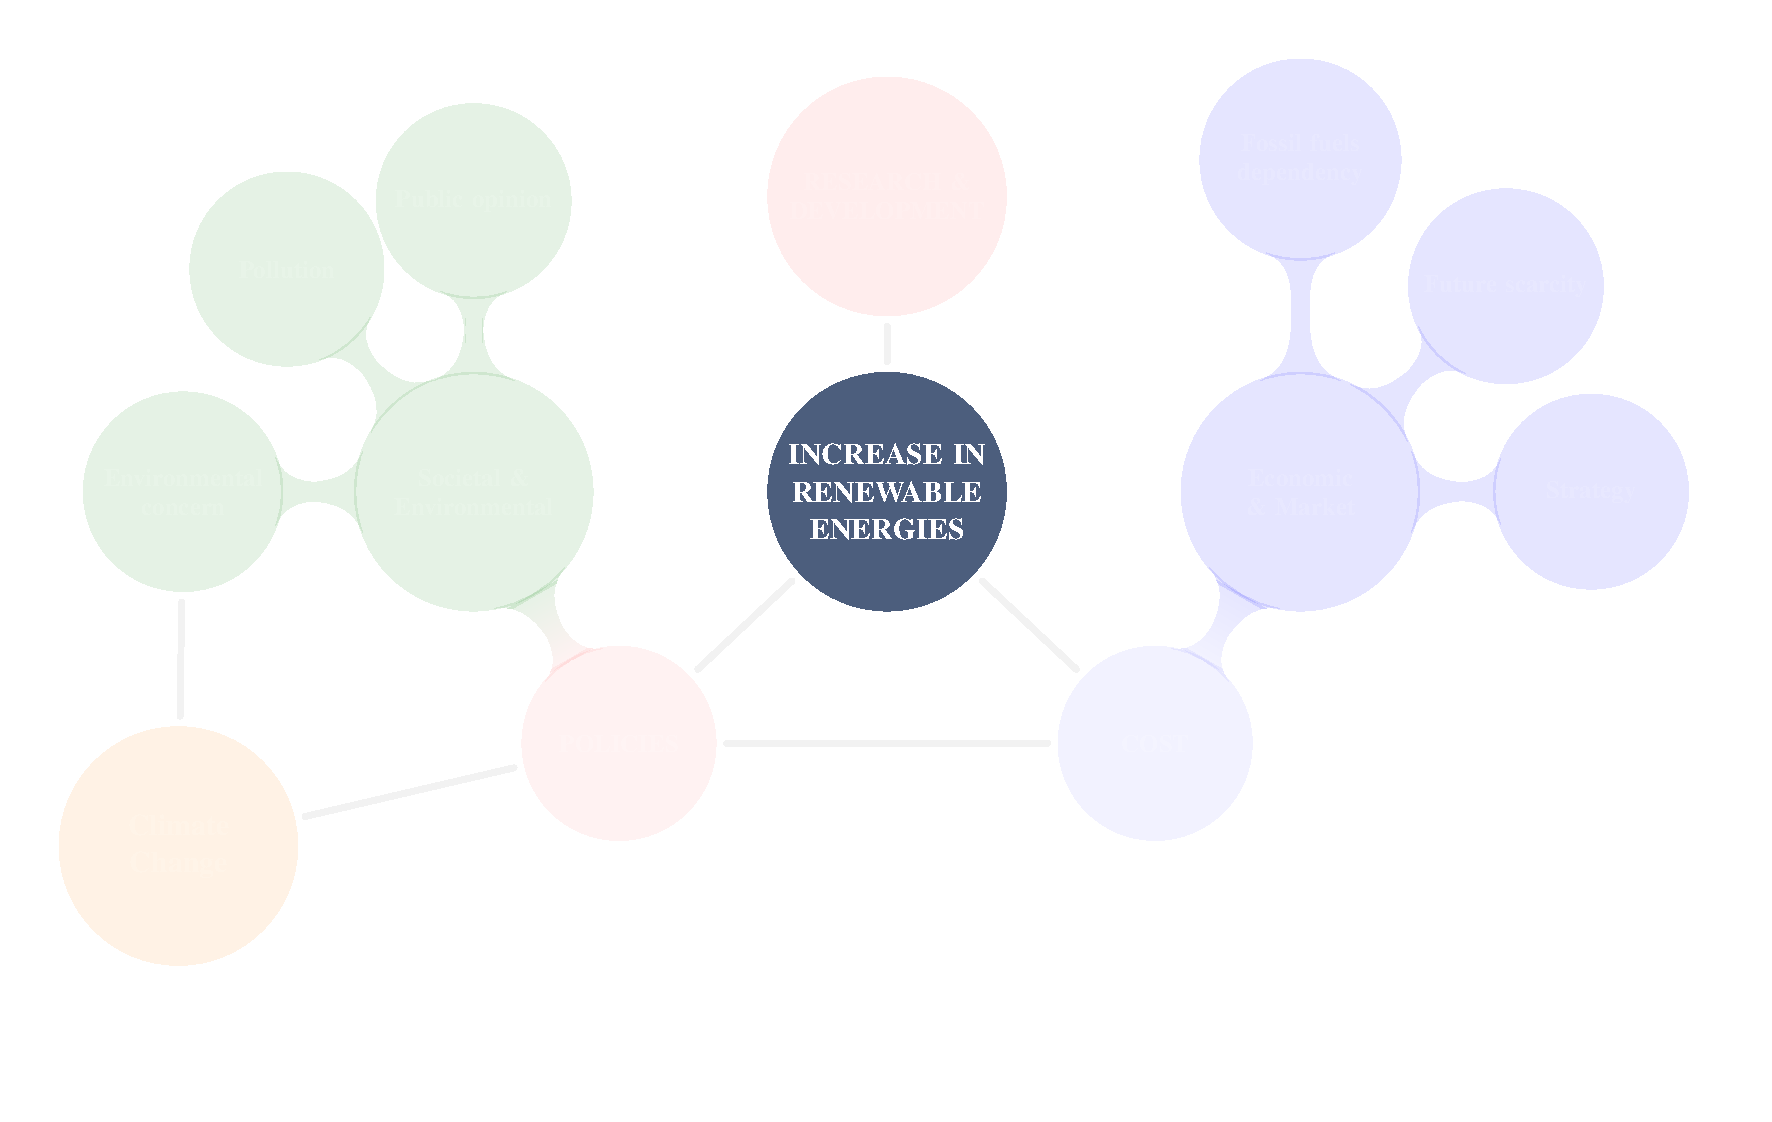
\includegraphics[scale=0.4]{diagram0.pdf}
\end{figure} 
\end{frame}


\begin{frame}[fragile]{Energy transition}
\begin{figure}
\centering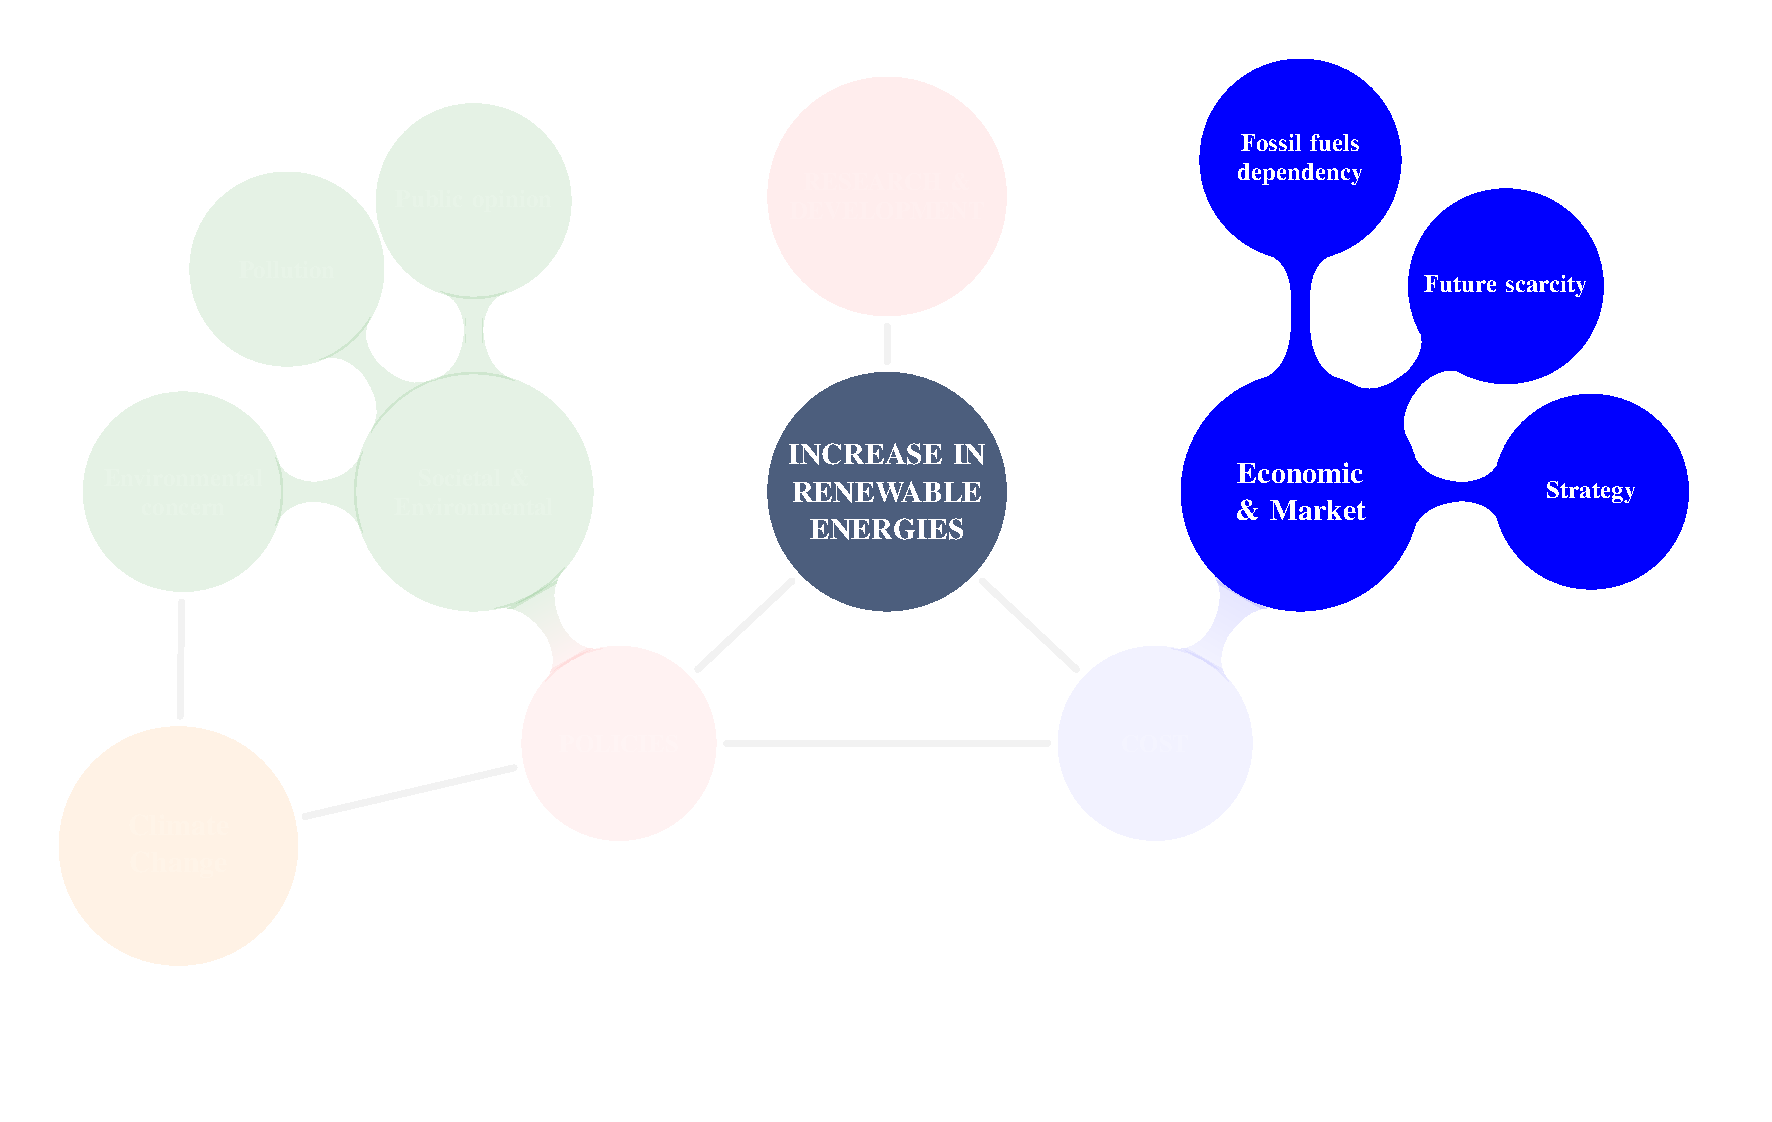
\includegraphics[scale=0.4]{diagrama1.pdf}
\end{figure} 
\end{frame}

\begin{frame}[fragile]{Energy transition}
\begin{figure}
\centering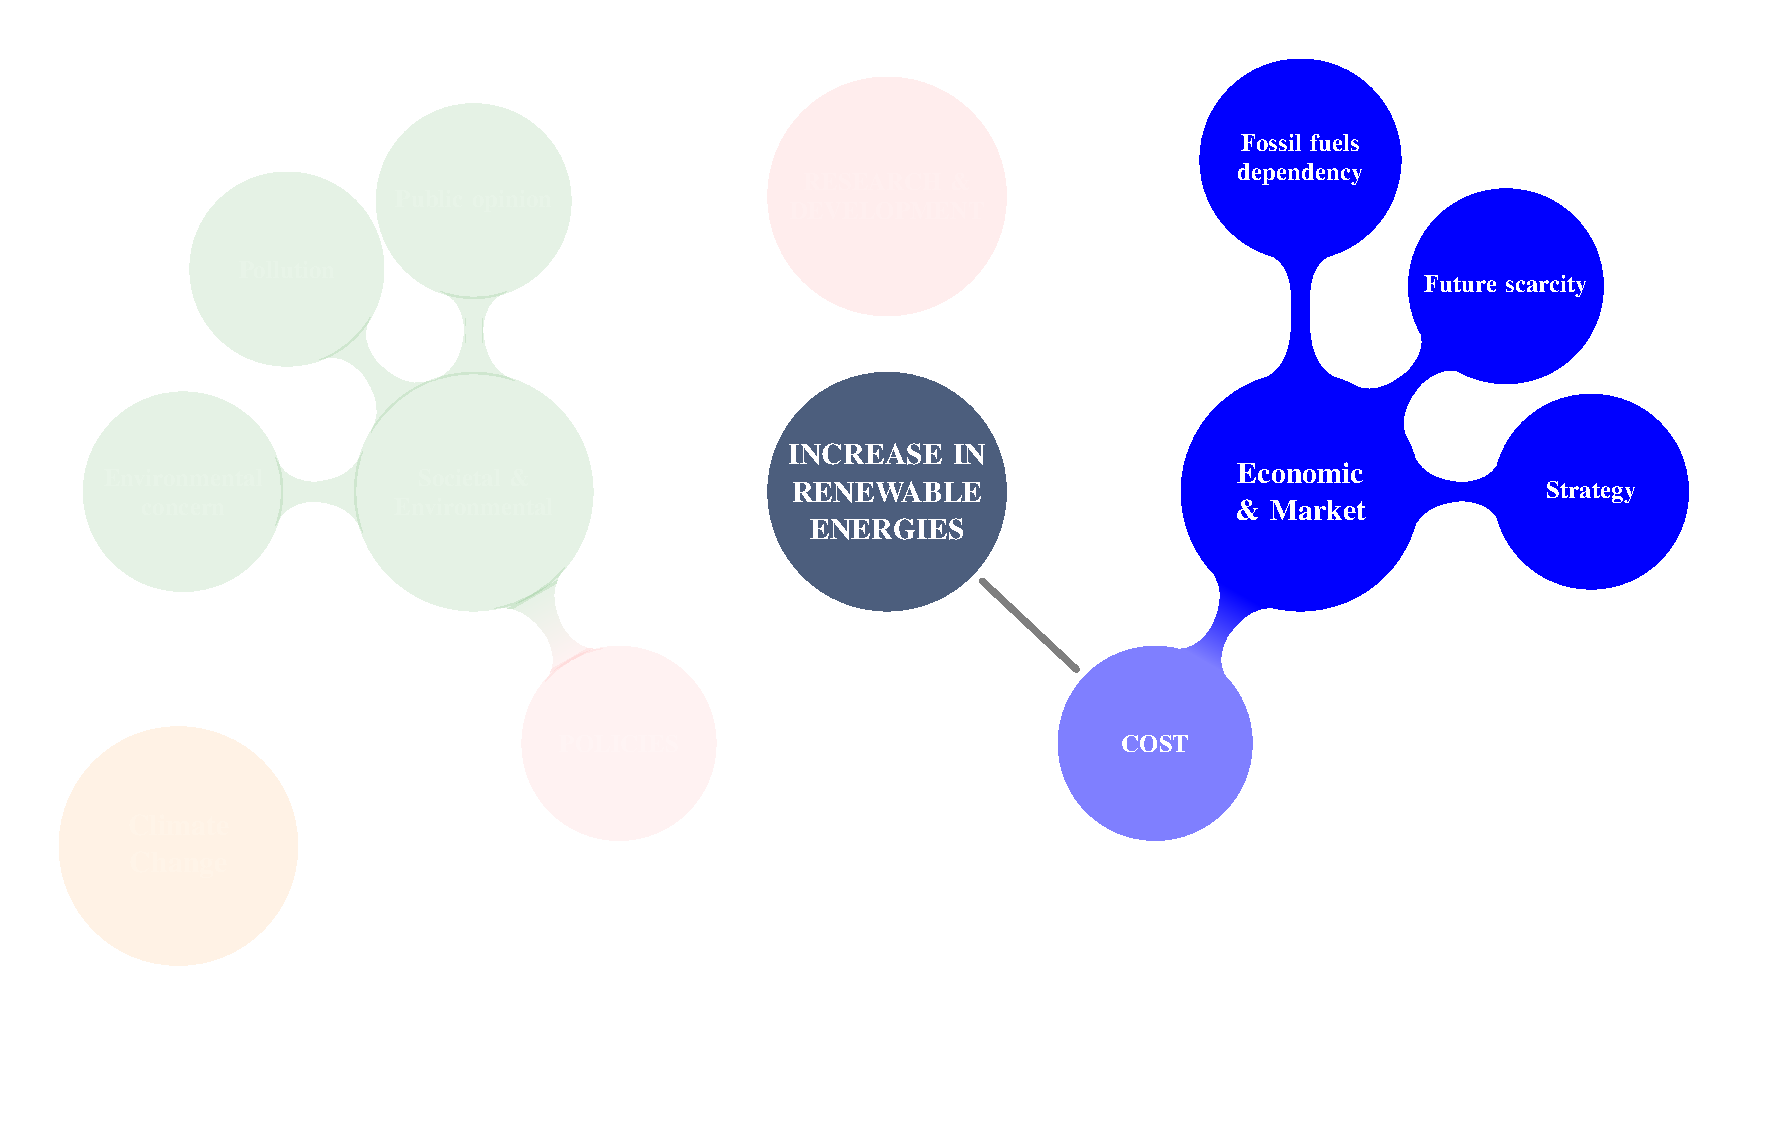
\includegraphics[scale=0.4]{diagrama2.pdf}
\end{figure} 
\end{frame}

\begin{frame}[fragile]{Energy transition}
\begin{figure}
\centering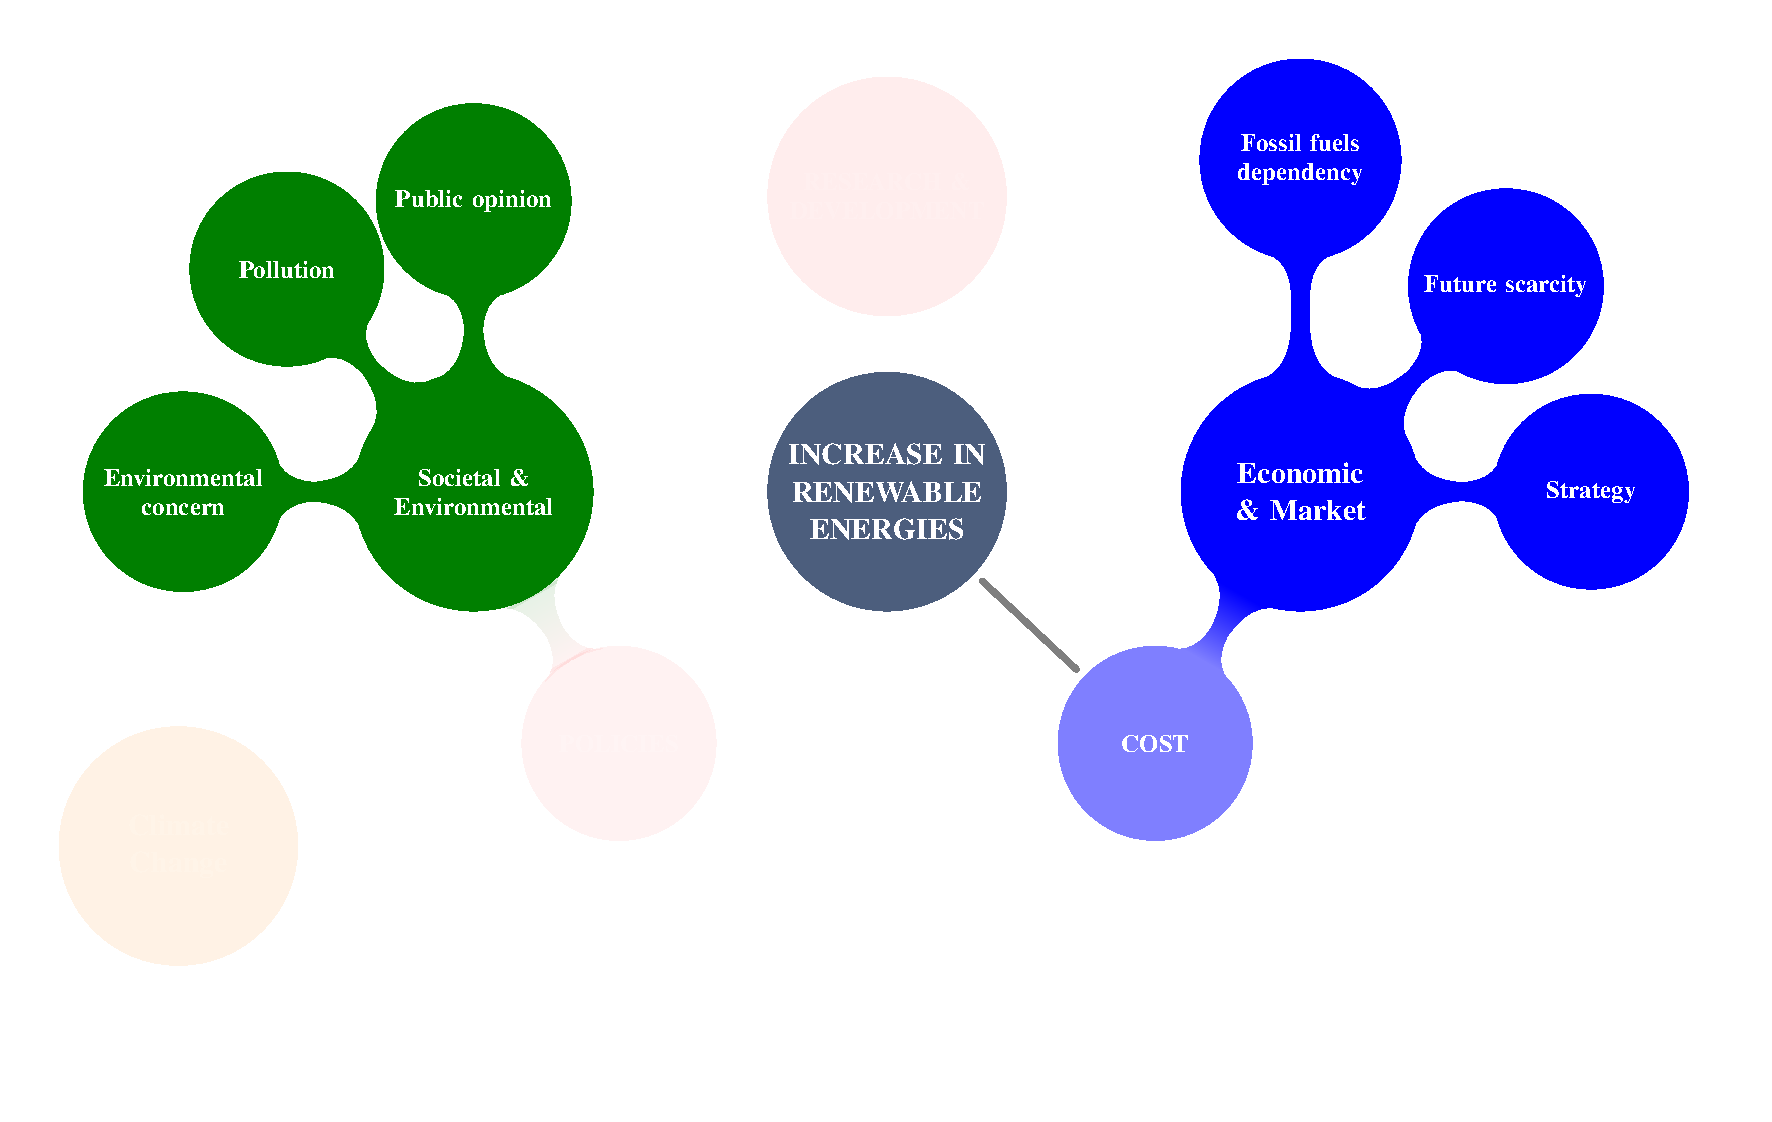
\includegraphics[scale=0.4]{diagrama3.pdf}
\end{figure} 
\end{frame}

\begin{frame}[fragile]{Energy transition}
\begin{figure}
\centering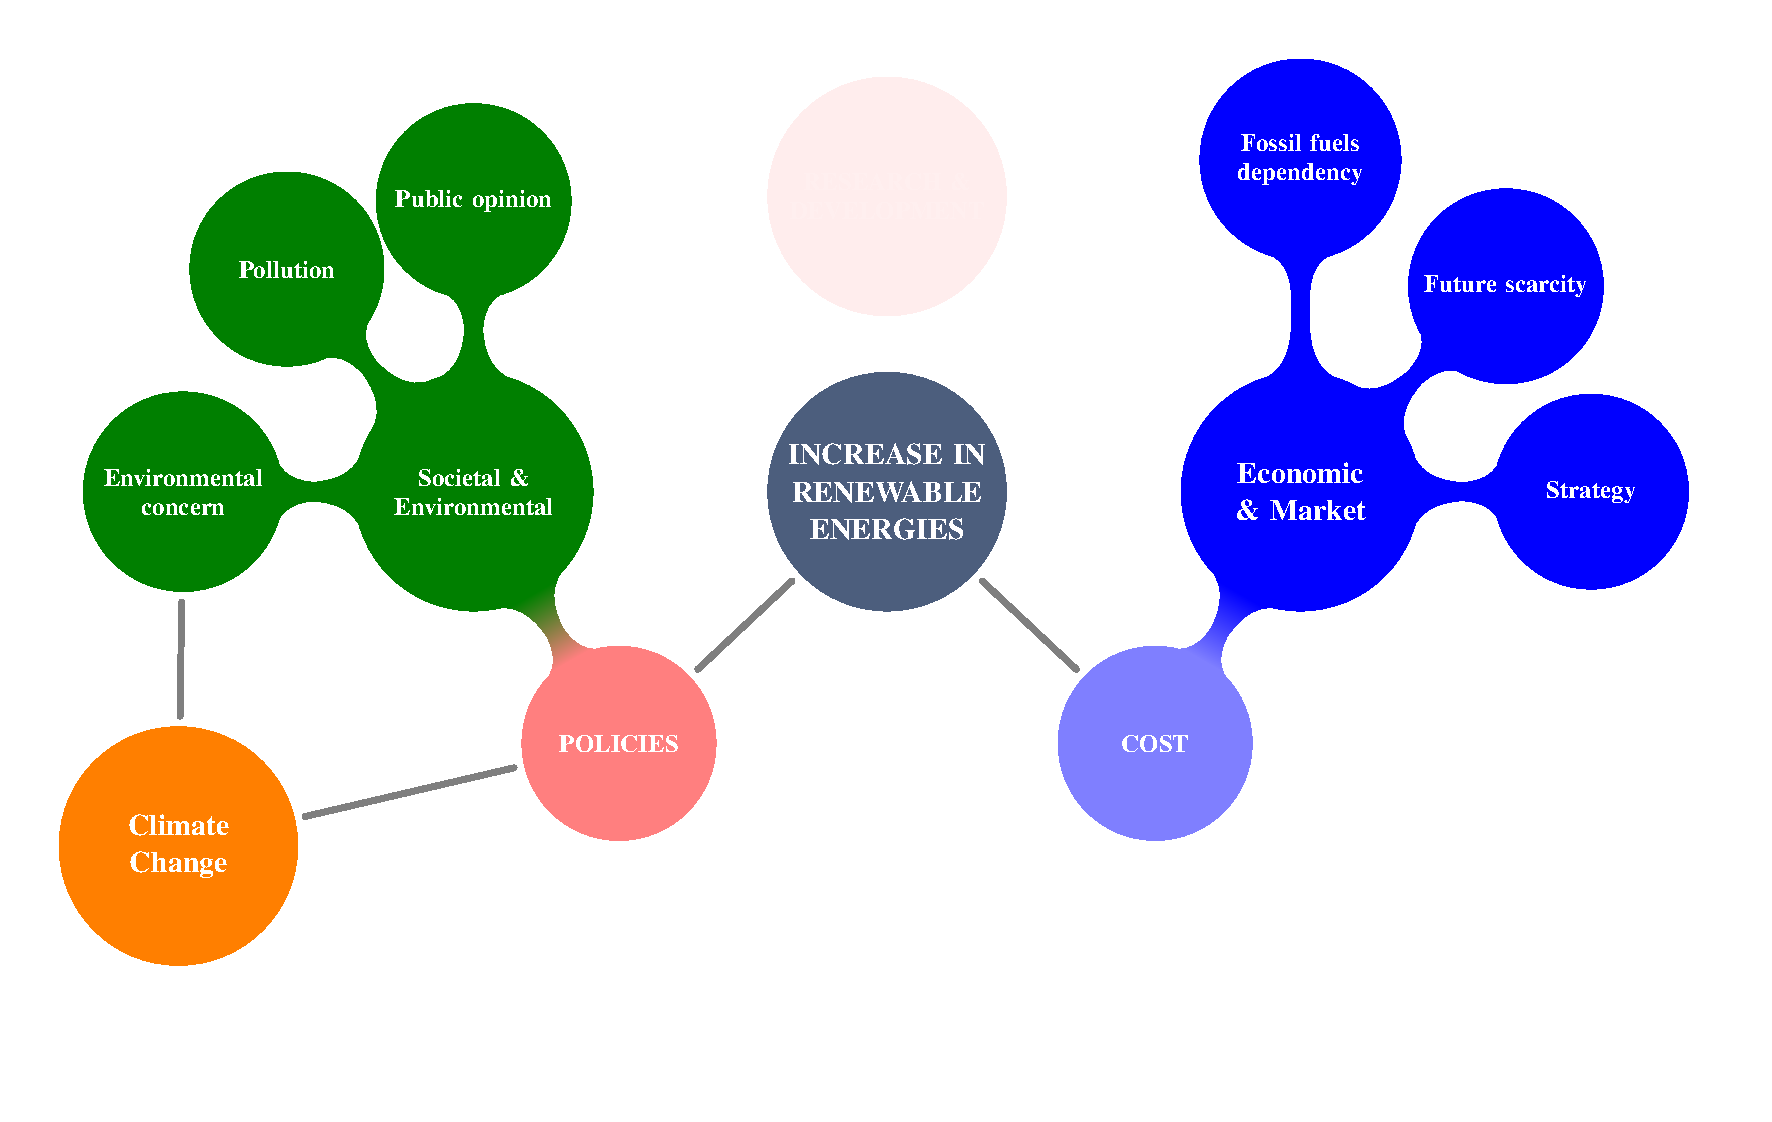
\includegraphics[scale=0.4]{diagrama4.pdf}
\end{figure} 
\end{frame}

\begin{frame}[fragile]{Energy transition}
\begin{figure}
\centering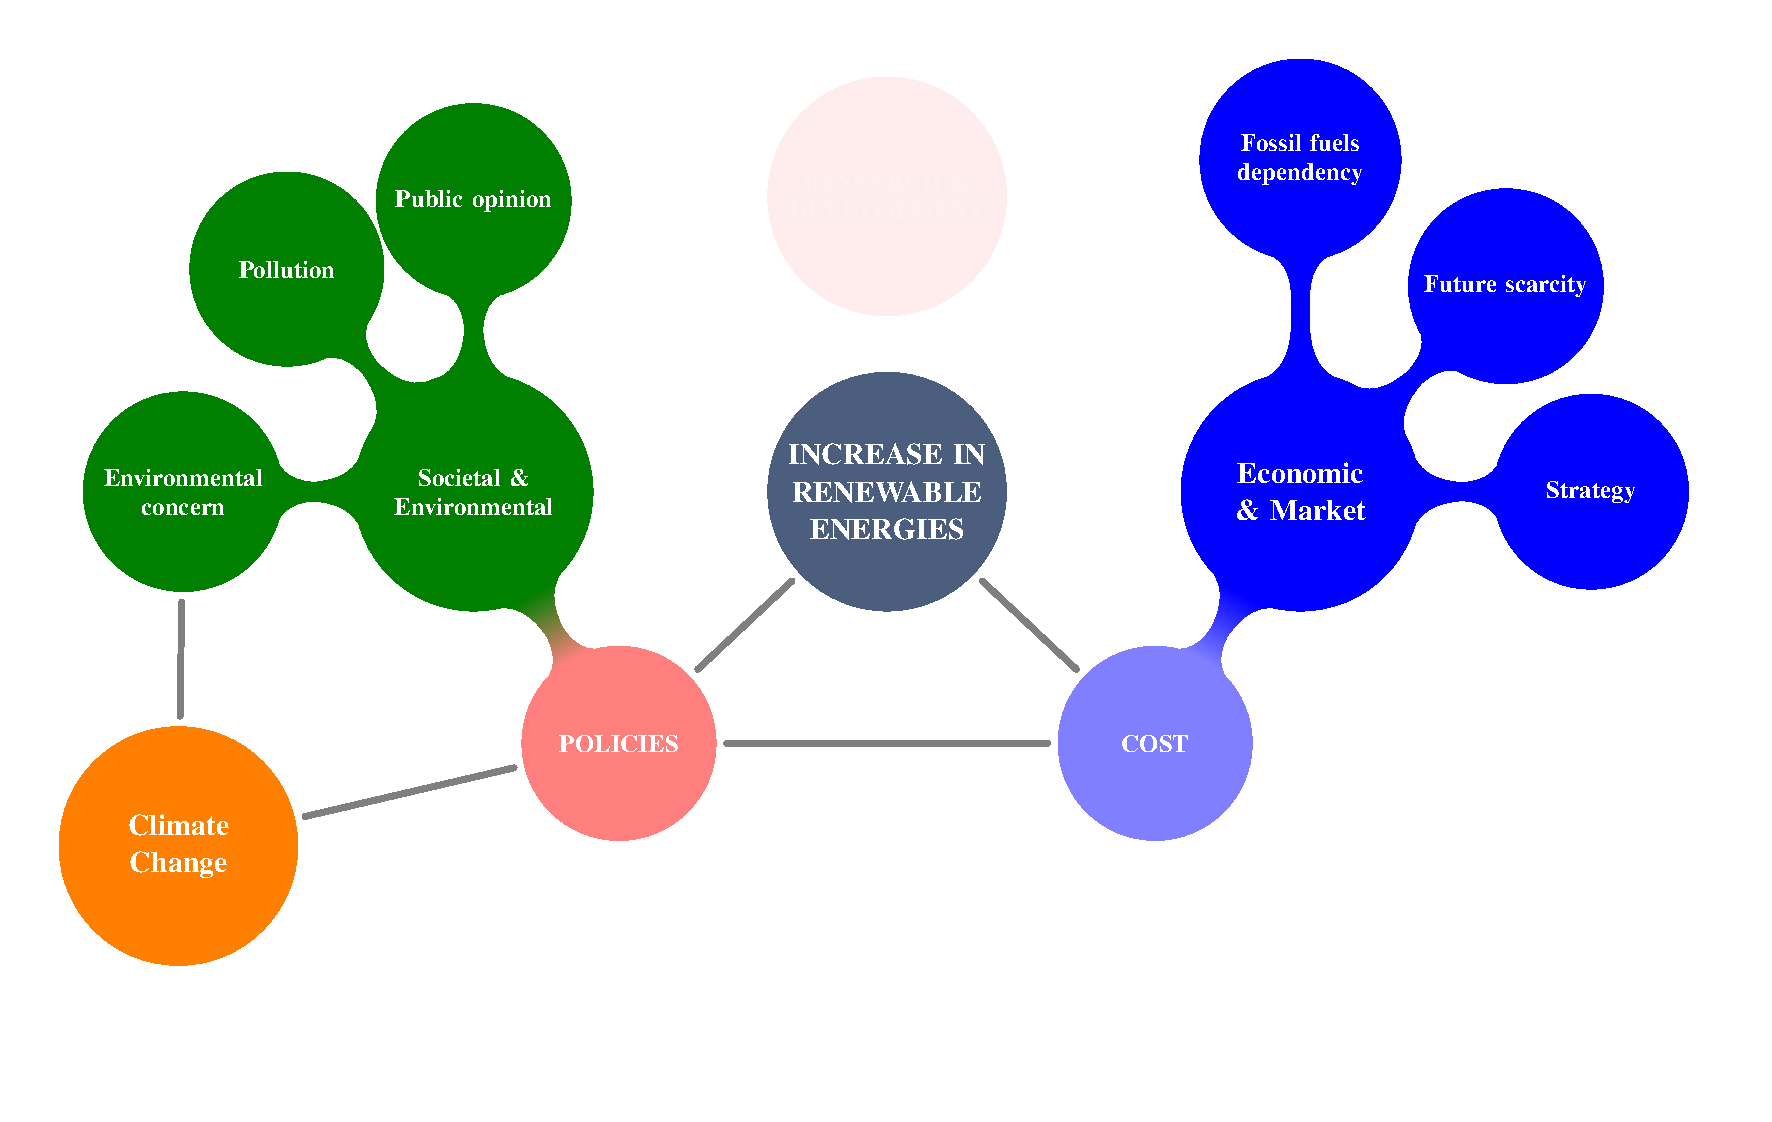
\includegraphics[scale=0.4]{diagrama5.pdf}
\end{figure} 
\end{frame}

\begin{frame}[fragile]{Energy transition}
\begin{figure}
\centering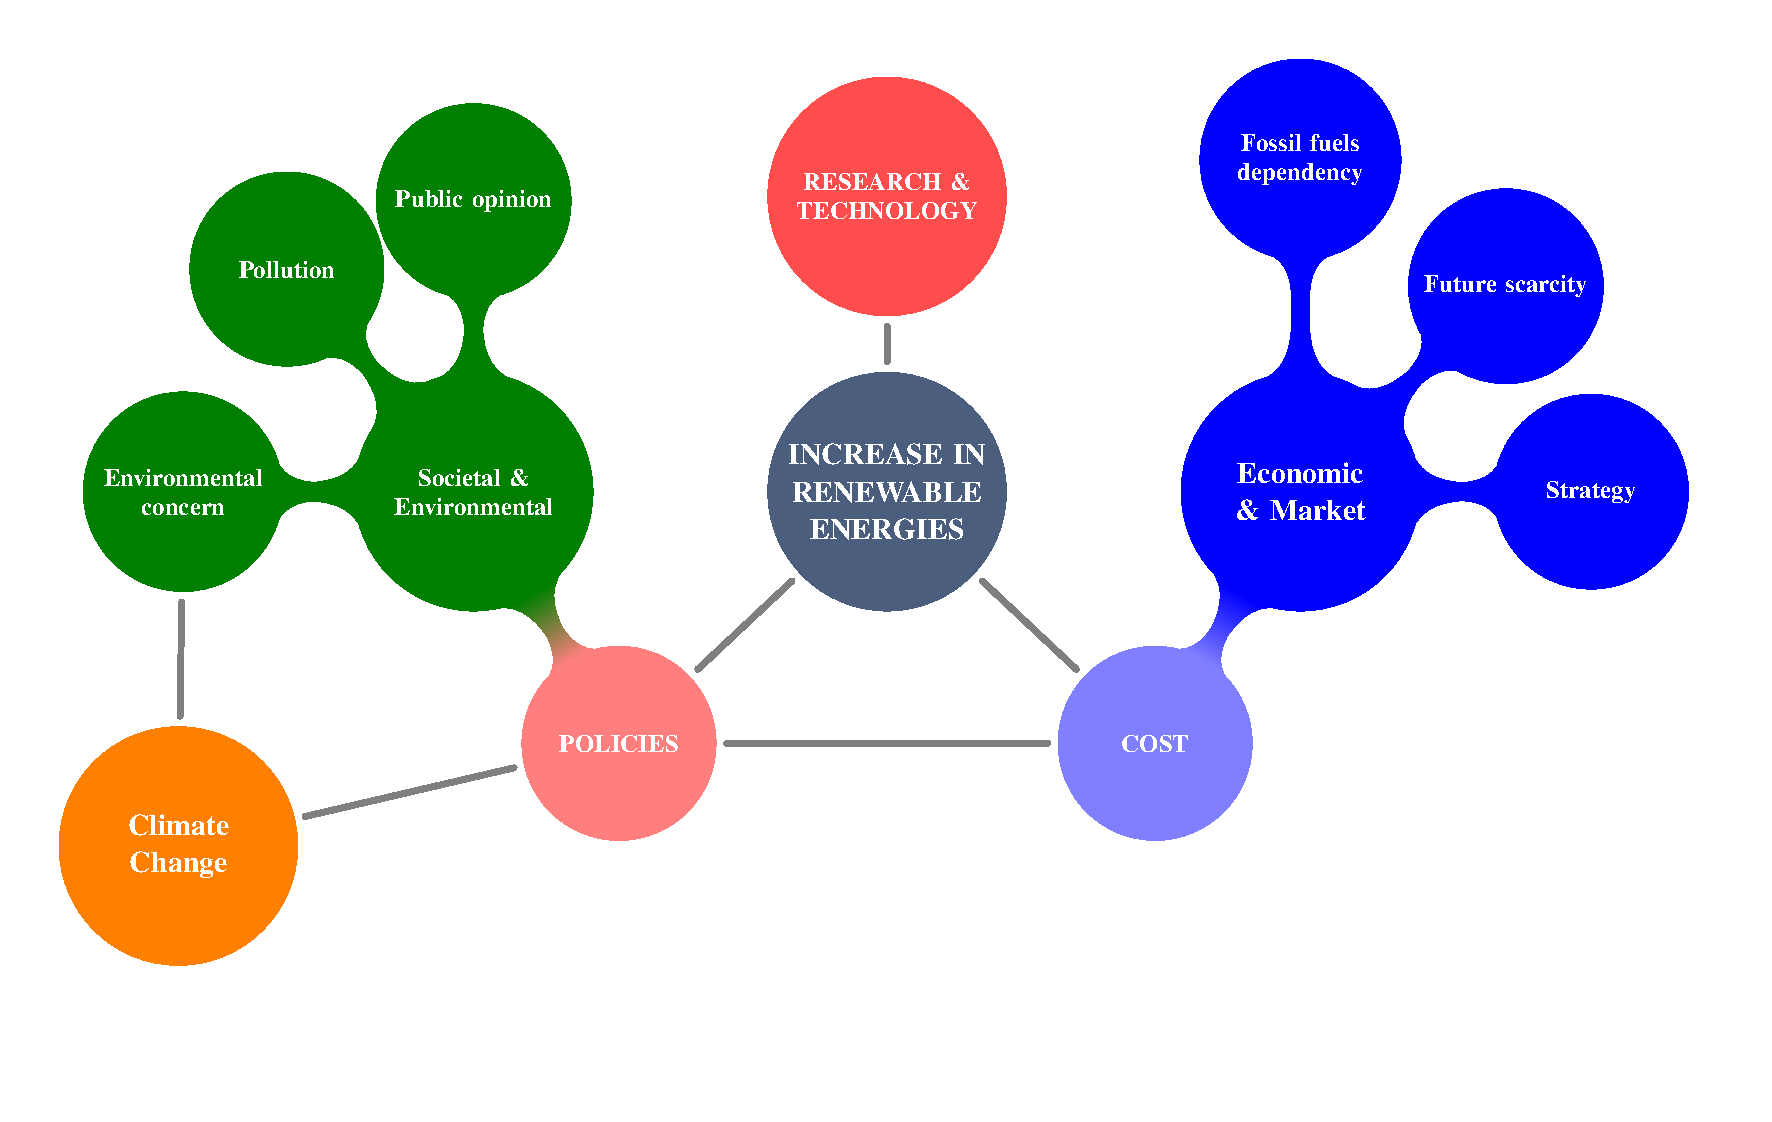
\includegraphics[scale=0.4]{diagram.pdf}
\end{figure} 
\end{frame}

\begin{frame}[fragile]{Photovoltaic}
\begin{itemize}
\item Increase in \textbf{\alert{photovoltaic (PV) capacity}}
\item Continous growth in projected \textbf{\alert{trends}}.
\item Global increase leaded by China  
\end{itemize}
\begin{figure}
\centering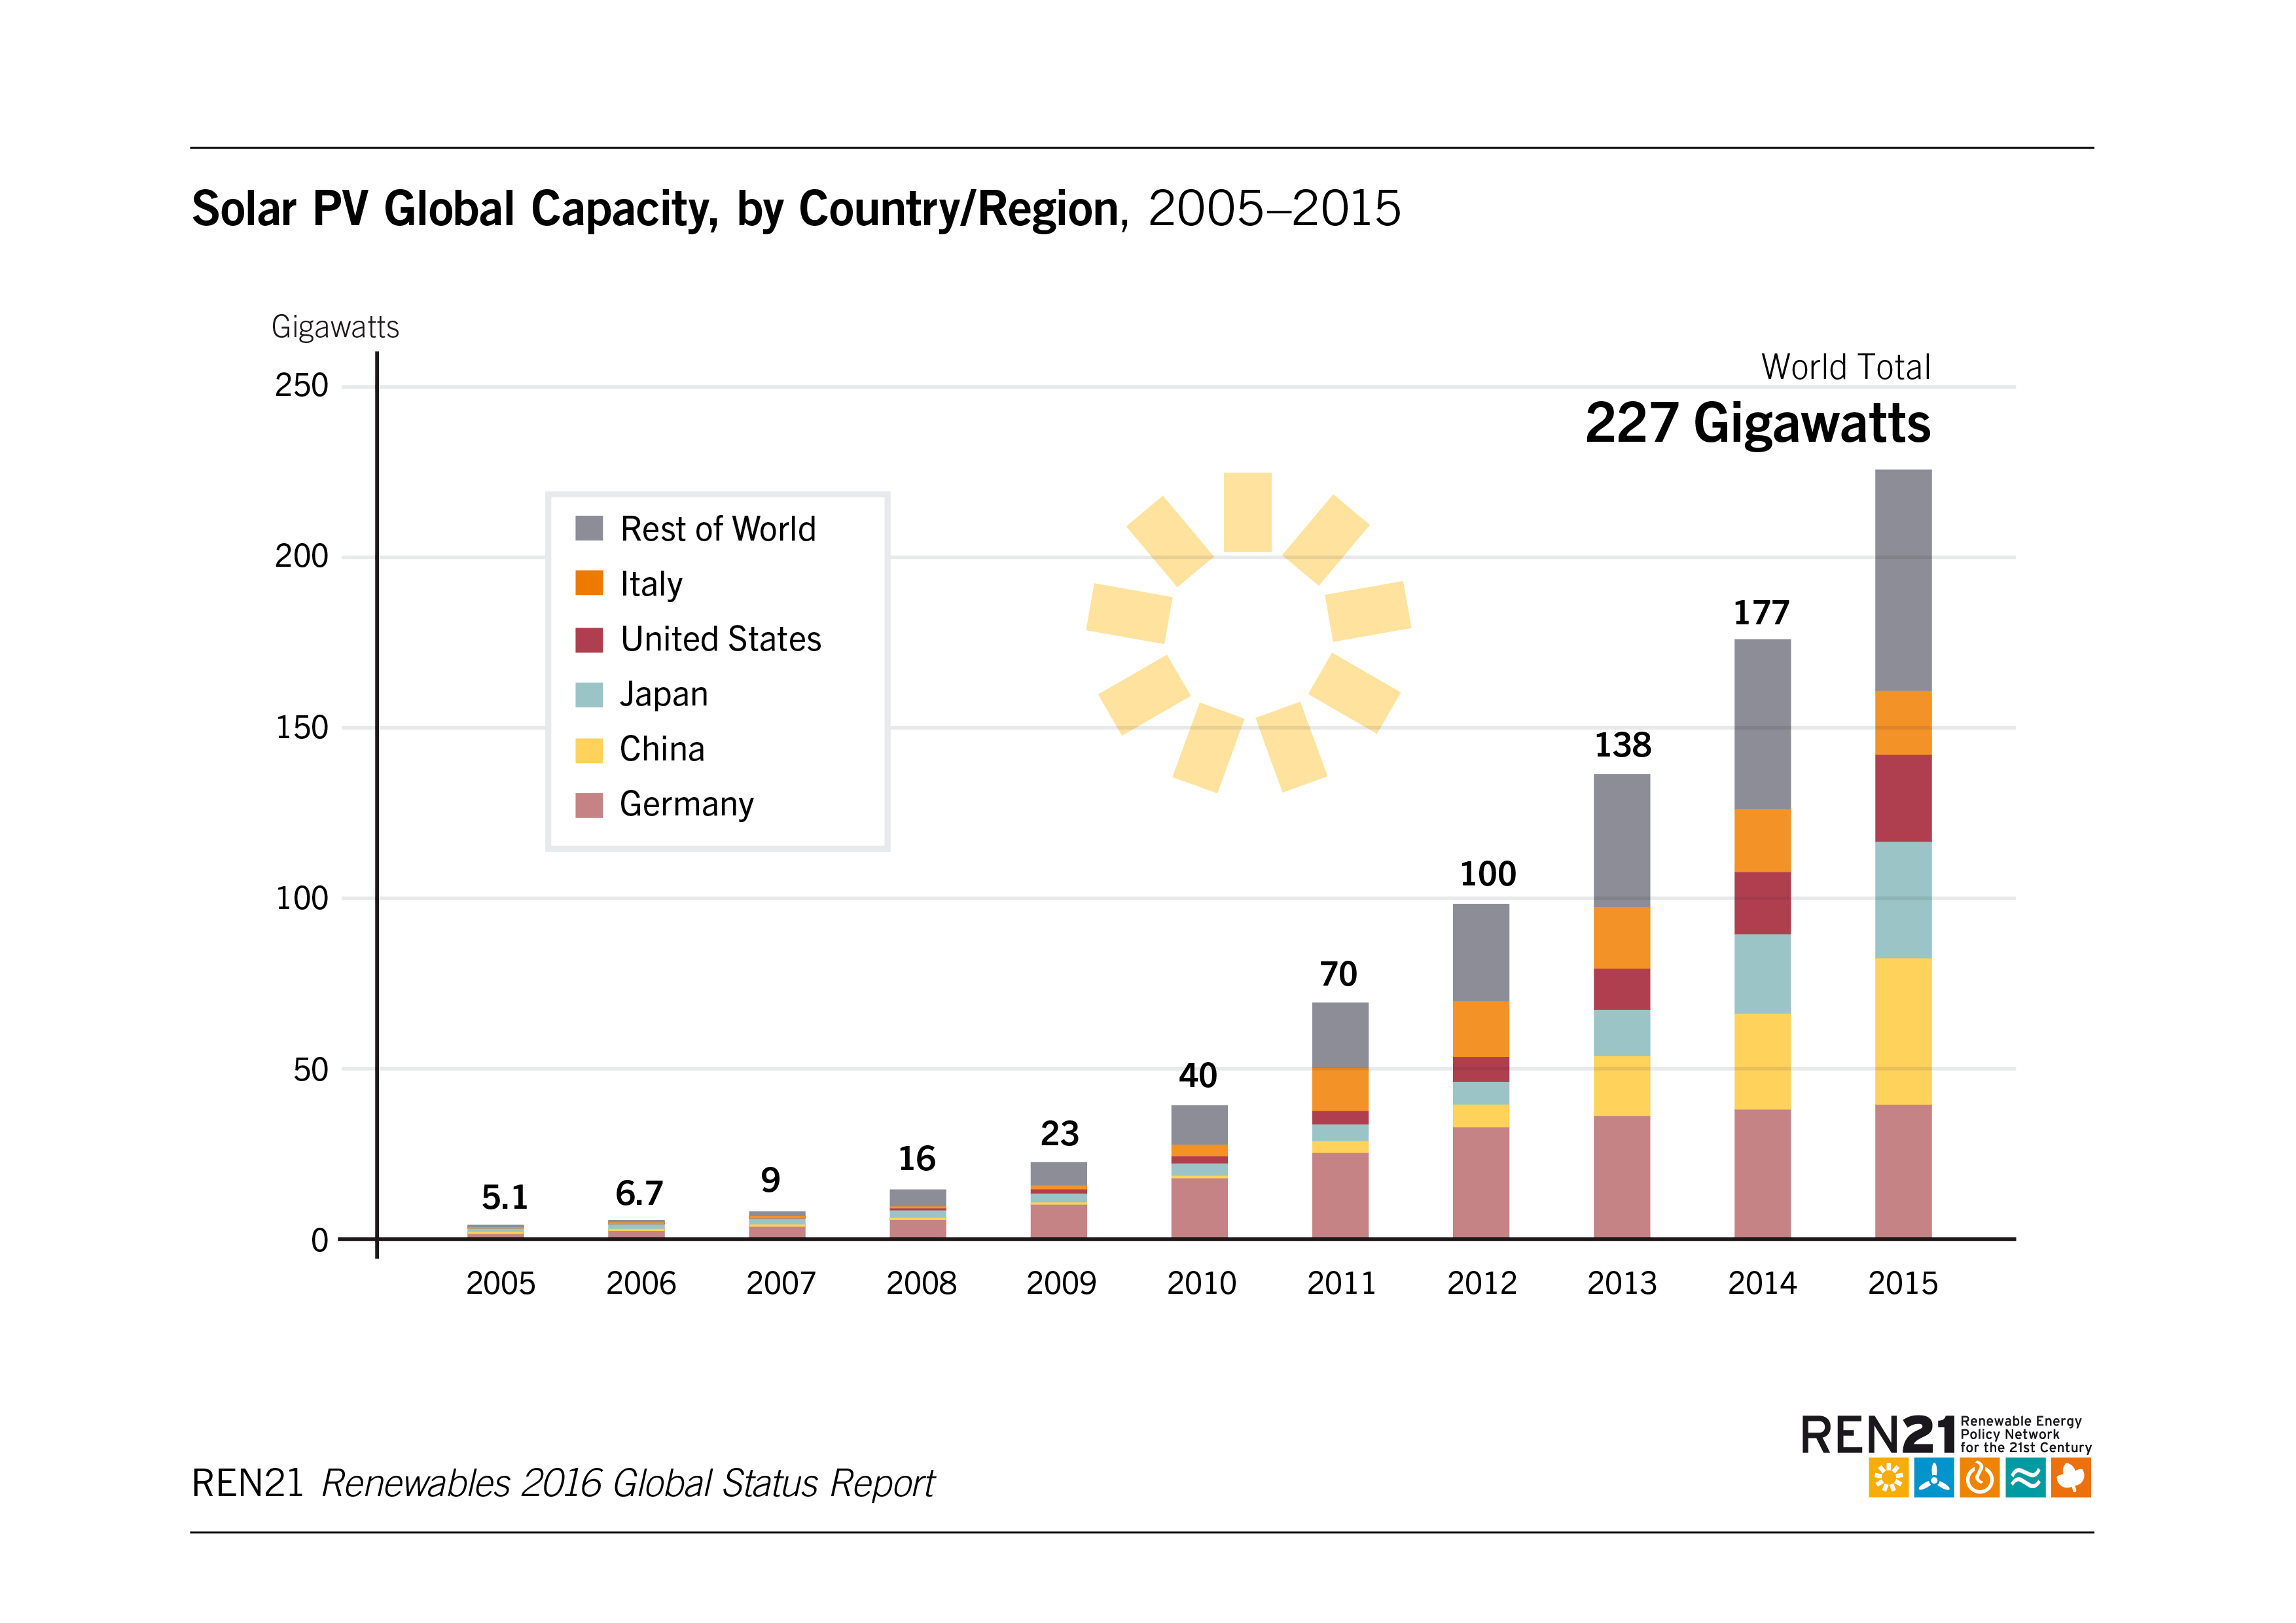
\includegraphics[scale=0.3]{GSR_2016_Figure_15}
\end{figure}
\end{frame}

\begin{frame}[fragile]{Links between climate/weather and the power sector}
\centering{\textbf{Increase in RE -> increase in the \alert{electrification} of the energy sector. }}
  \begin{columns}
    \begin{column}{0.3\textwidth}
  \begin{figure}
    \centering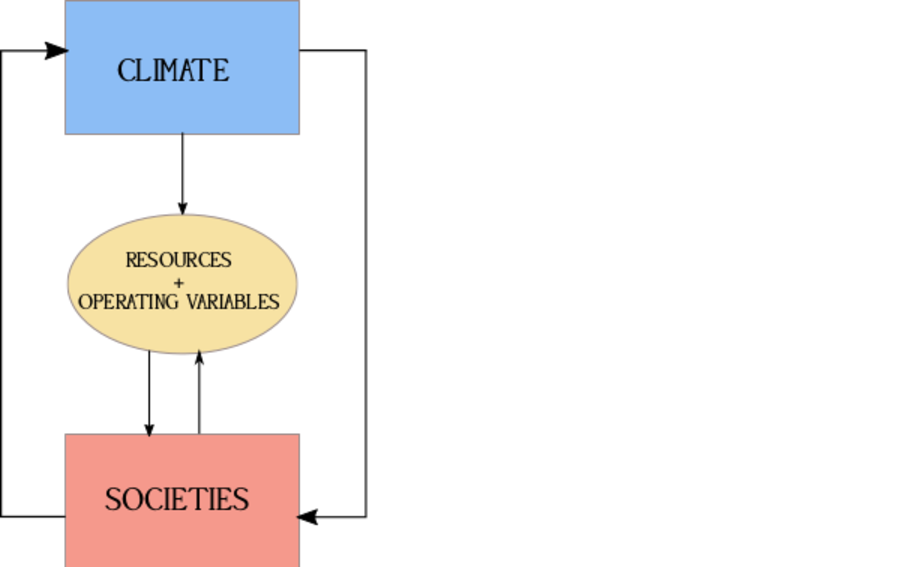
\includegraphics[scale=0.55]{drawing1.pdf}
\end{figure}
  \end{column}
  \begin{column}{0.7\textwidth}
    \begin{itemize}
    \item Highly dependent on the state of the atmosphere:
      \begin{itemize}
      \item <2->\textbf{\alert{supply side}}: potential energy produced/ mean resource with RE
      \item <3->\textbf{\alert{demand side}}: Modulate the electricity demand
      \item <4->Operating variables: temperature   
      \end{itemize}
      \end{itemize}
    \end{column}
    \end{columns}
\end{frame}

\begin{frame}[fragile]{Links between climate/weather and the power sector}
\centering{\textbf{Increase in RE -> increase in the \alert{electrification} of the energy sector. }}
  \begin{columns}
    \begin{column}{0.7\textwidth}
  \begin{figure}
    \centering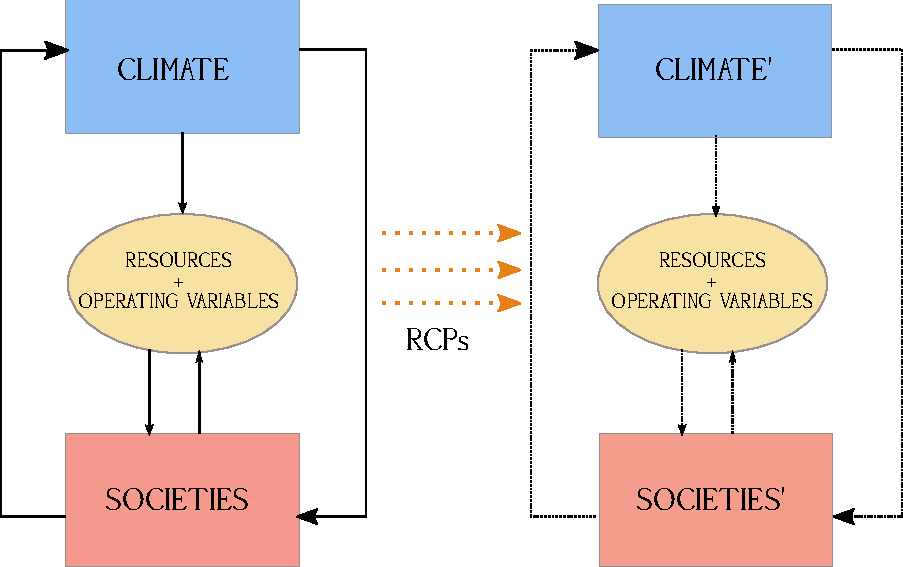
\includegraphics[scale=0.55]{drawing.pdf}
\end{figure}
  \end{column}
  \begin{column}{0.3\textwidth}
    % \begin{itemize}
    % \item Changes in the supply side
    %  \item Changes in the demand side 
    %   \end{itemize}
    \end{column}
    \end{columns}
\end{frame}

\begin{frame}[fragile]{Links between climate/weather and the porwe sector}
\centering{\textbf{Increase in RE -> increase in the \alert{electrification} of the energy sector. }}
  \begin{columns}
    \begin{column}{0.7\textwidth}
  \begin{figure}
    \centering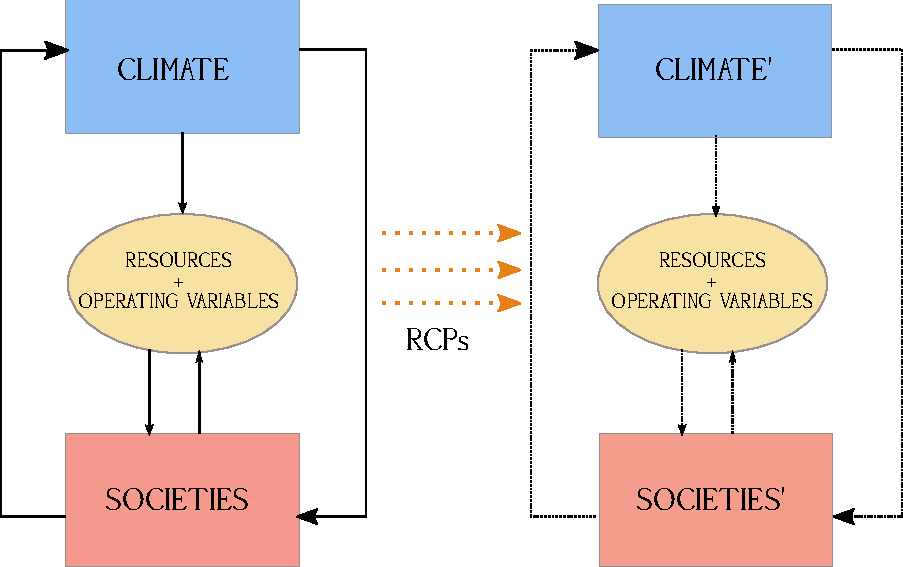
\includegraphics[scale=0.55]{drawing.pdf}
\end{figure}
  \end{column}
  \begin{column}{0.3\textwidth}
\small{    \begin{itemize}
    \item Changes in the \alert{supply} side
     \item Changes in the \alert{demand} side 
      \end{itemize}}
    \end{column}
    \end{columns}
\end{frame}


\subsection{VRE}
 
% {
% \usebackgroundtemplate{\tikz\node[opacity=1, inner sep=0pt, outer sep=0pt]{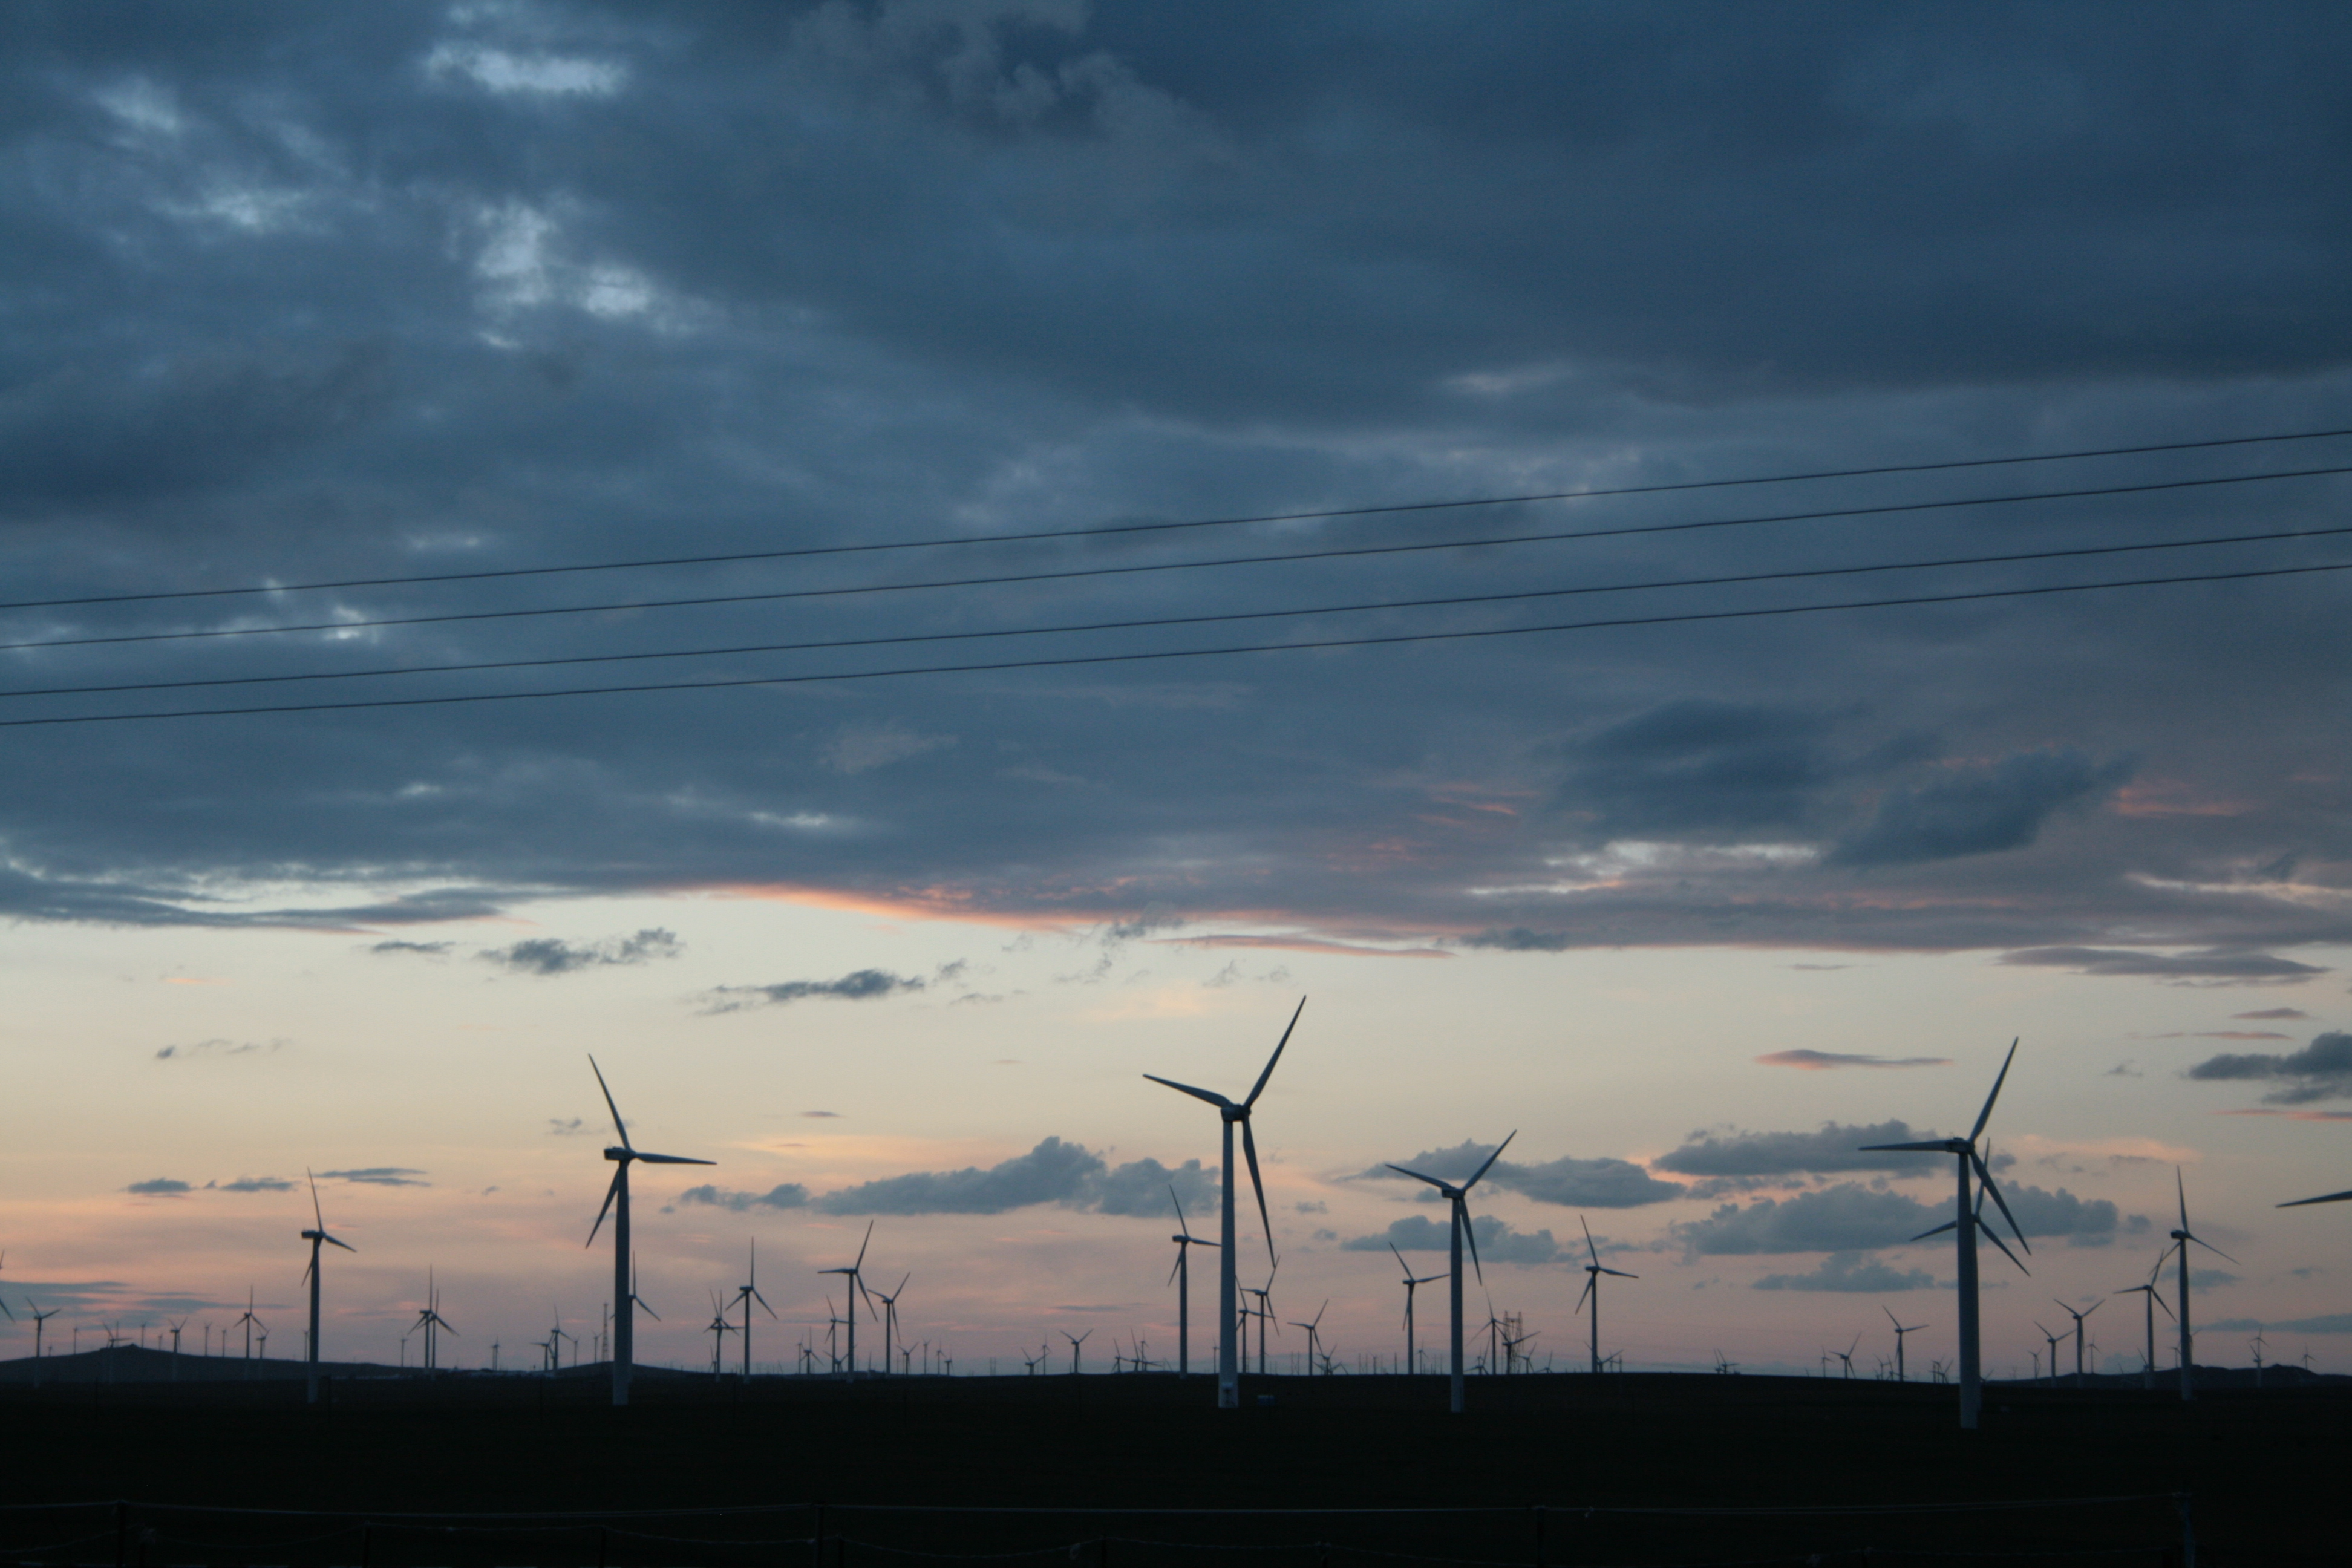
\includegraphics[width=\paperwidth, height=1.1\paperheight]{aeromongolia.JPG}};}
% \begin{frame}{RE in the electricity system}
% \begin{alertblock}  
% \begin{itemize}
%   \item{\textcolor{black}{Demand and supply need to be \textbf{\alert{balanced}}}.}
%   \item{\textcolor{black}{Electricity systems are designed for centralized \alert{conventional power plants}}.}
%   \item{\textcolor{black}{\textbf{\alert{VRE}}: variable renewable energy}}
%   \end{itemize}
% \end{alertblock}
% \end{frame}
% }

 
%{
%\usebackgroundtemplate{\tikz\node[opacity=1, inner sep=0pt, outer sep=0pt]{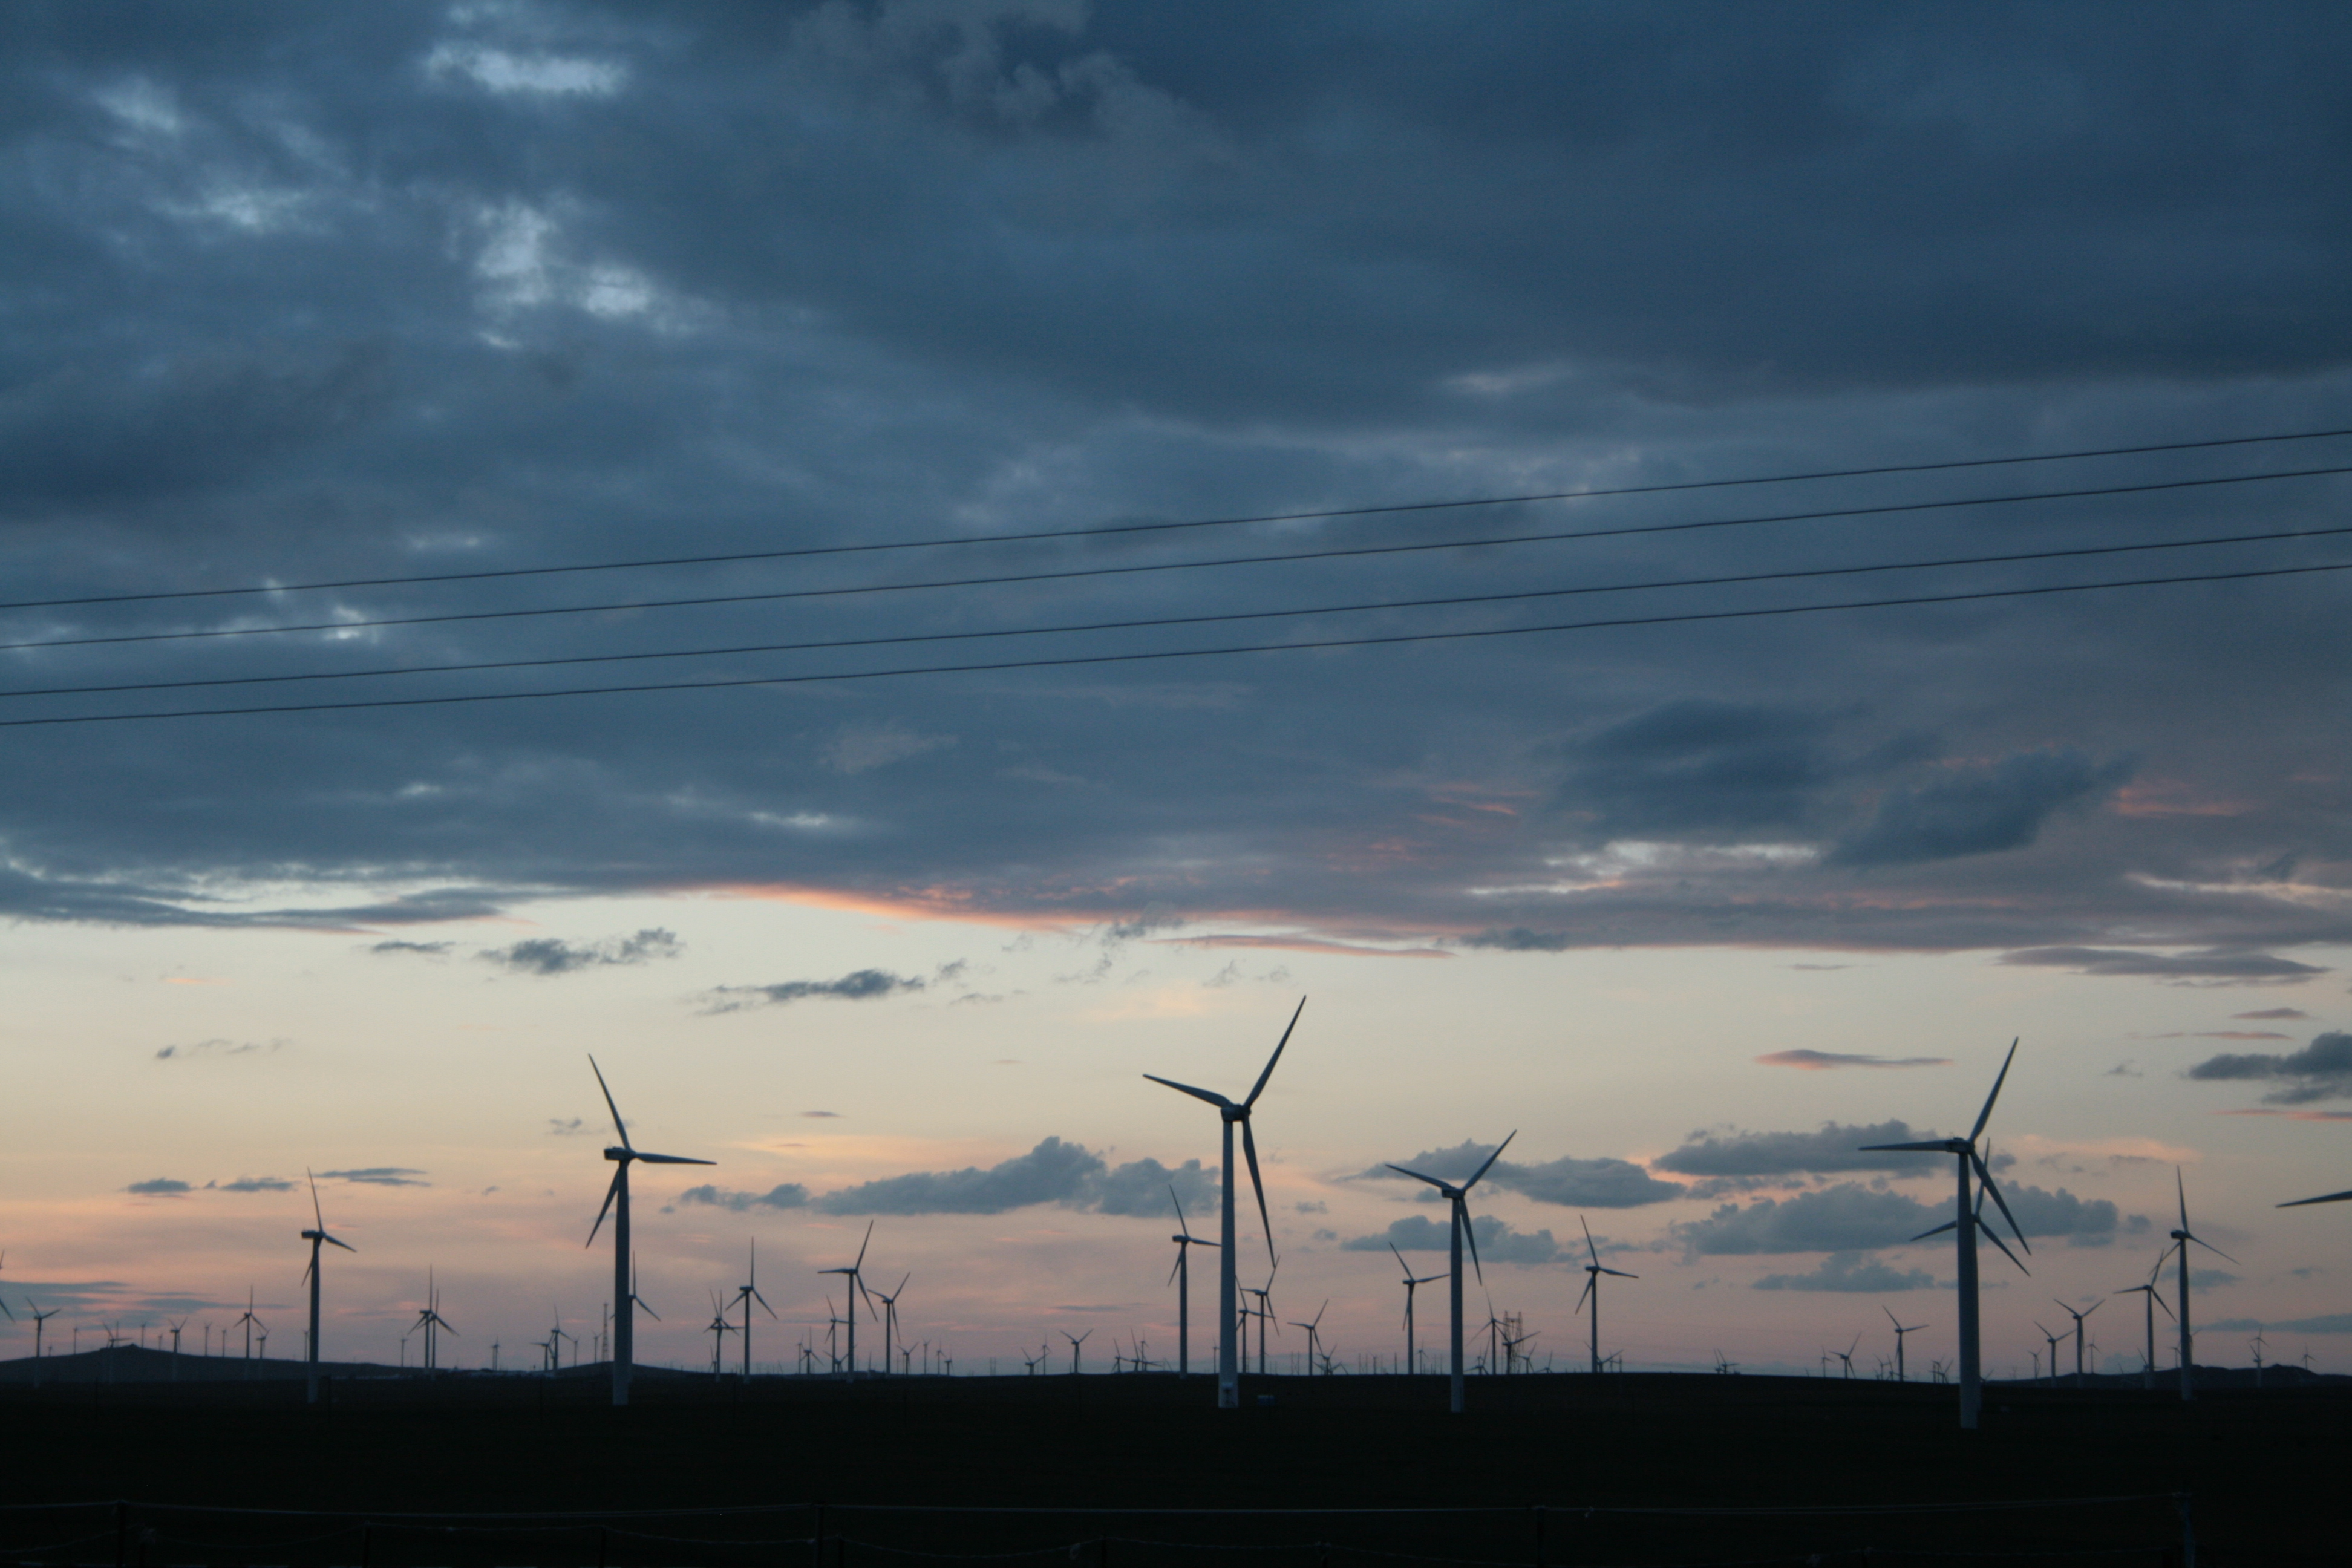
\includegraphics[width=\paperwidth, height=1.1\paperheight]{aeromongolia.JPG}};}
% \begin{frame}{RE in the electricity system}
% \begin{alertblock}
% \begin{itemize}  
%   \item Demand and supply need to be \alert{balanced}.
%   \item Electricity systems are designed for centralized \alert{conventional power plants}.
%   \item \alert{VRE}: variable renewable energy.
% \end{itemize}
% \end{alertblock}  
% \end{frame}
%}

% {
% \usebackgroundtemplate{\tikz\node[opacity=1, inner sep=0pt, outer sep=0pt]{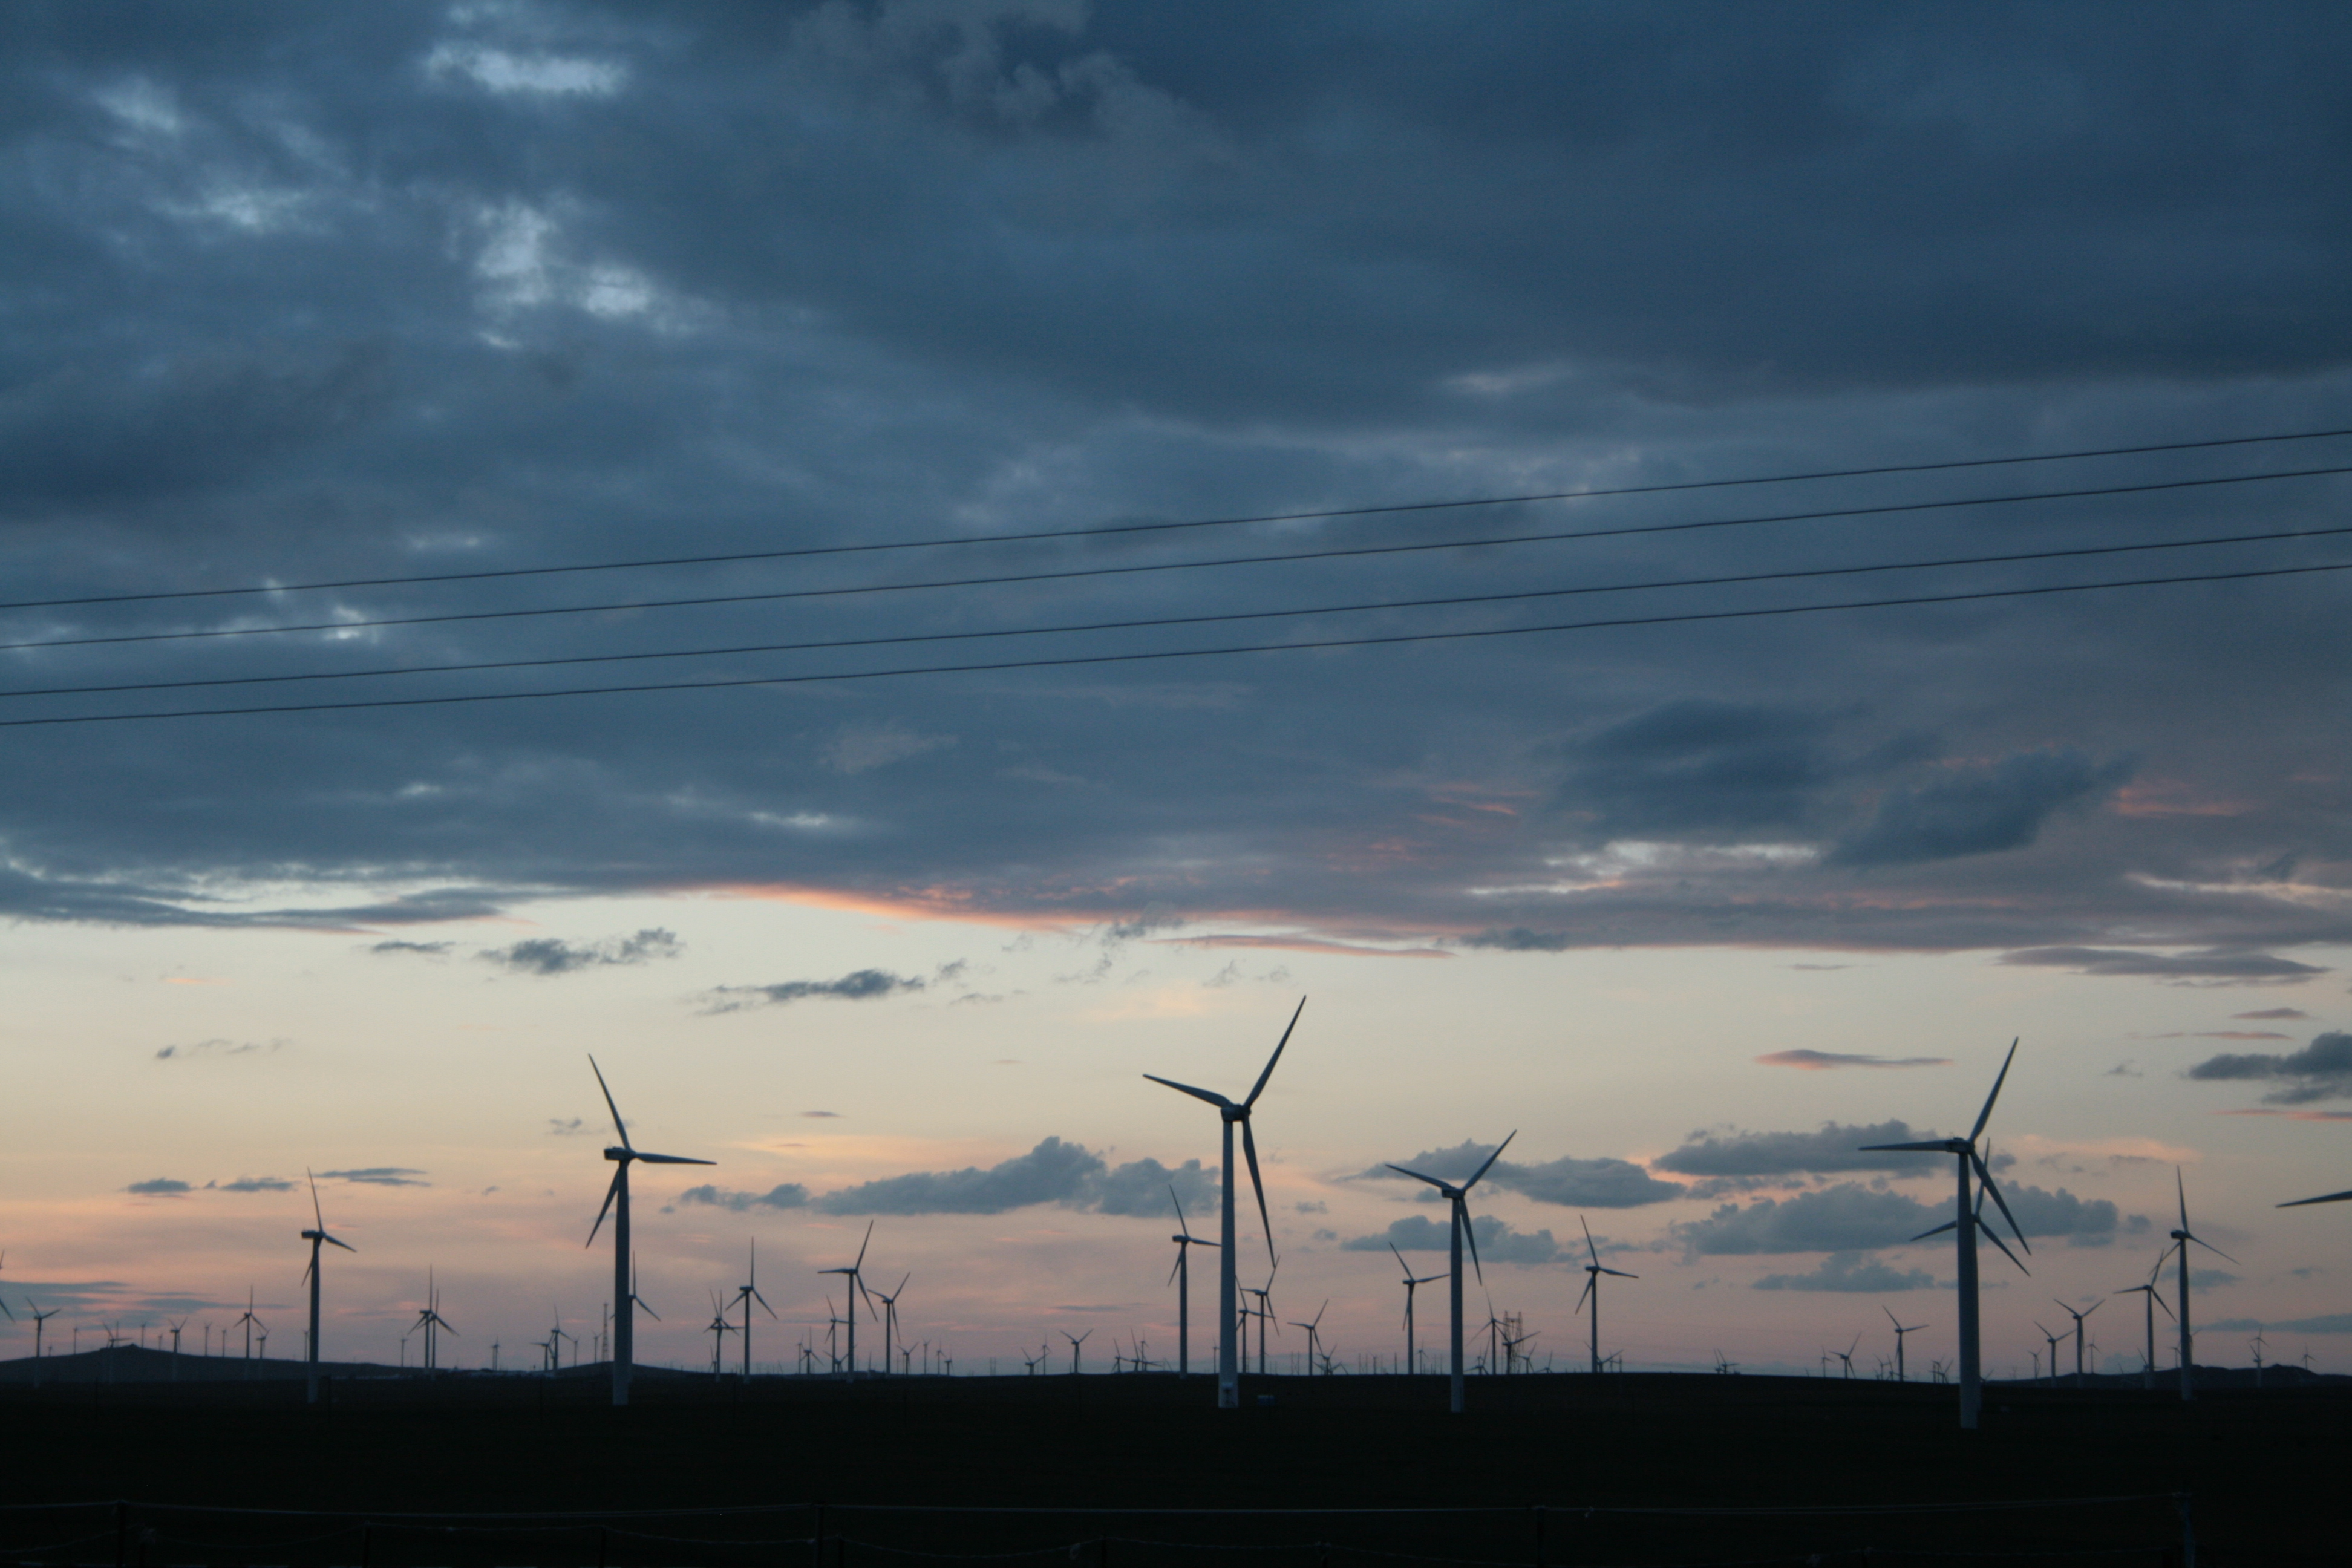
\includegraphics[width=\paperwidth, height=1.1\paperheight]{aeromongolia.JPG}};}
% \begin{frame}{RE in the electricity system}
% \end{frame}
% }

% {
% \usebackgroundtemplate{\tikz\node[opacity=1, inner sep=0pt, outer sep=0pt]{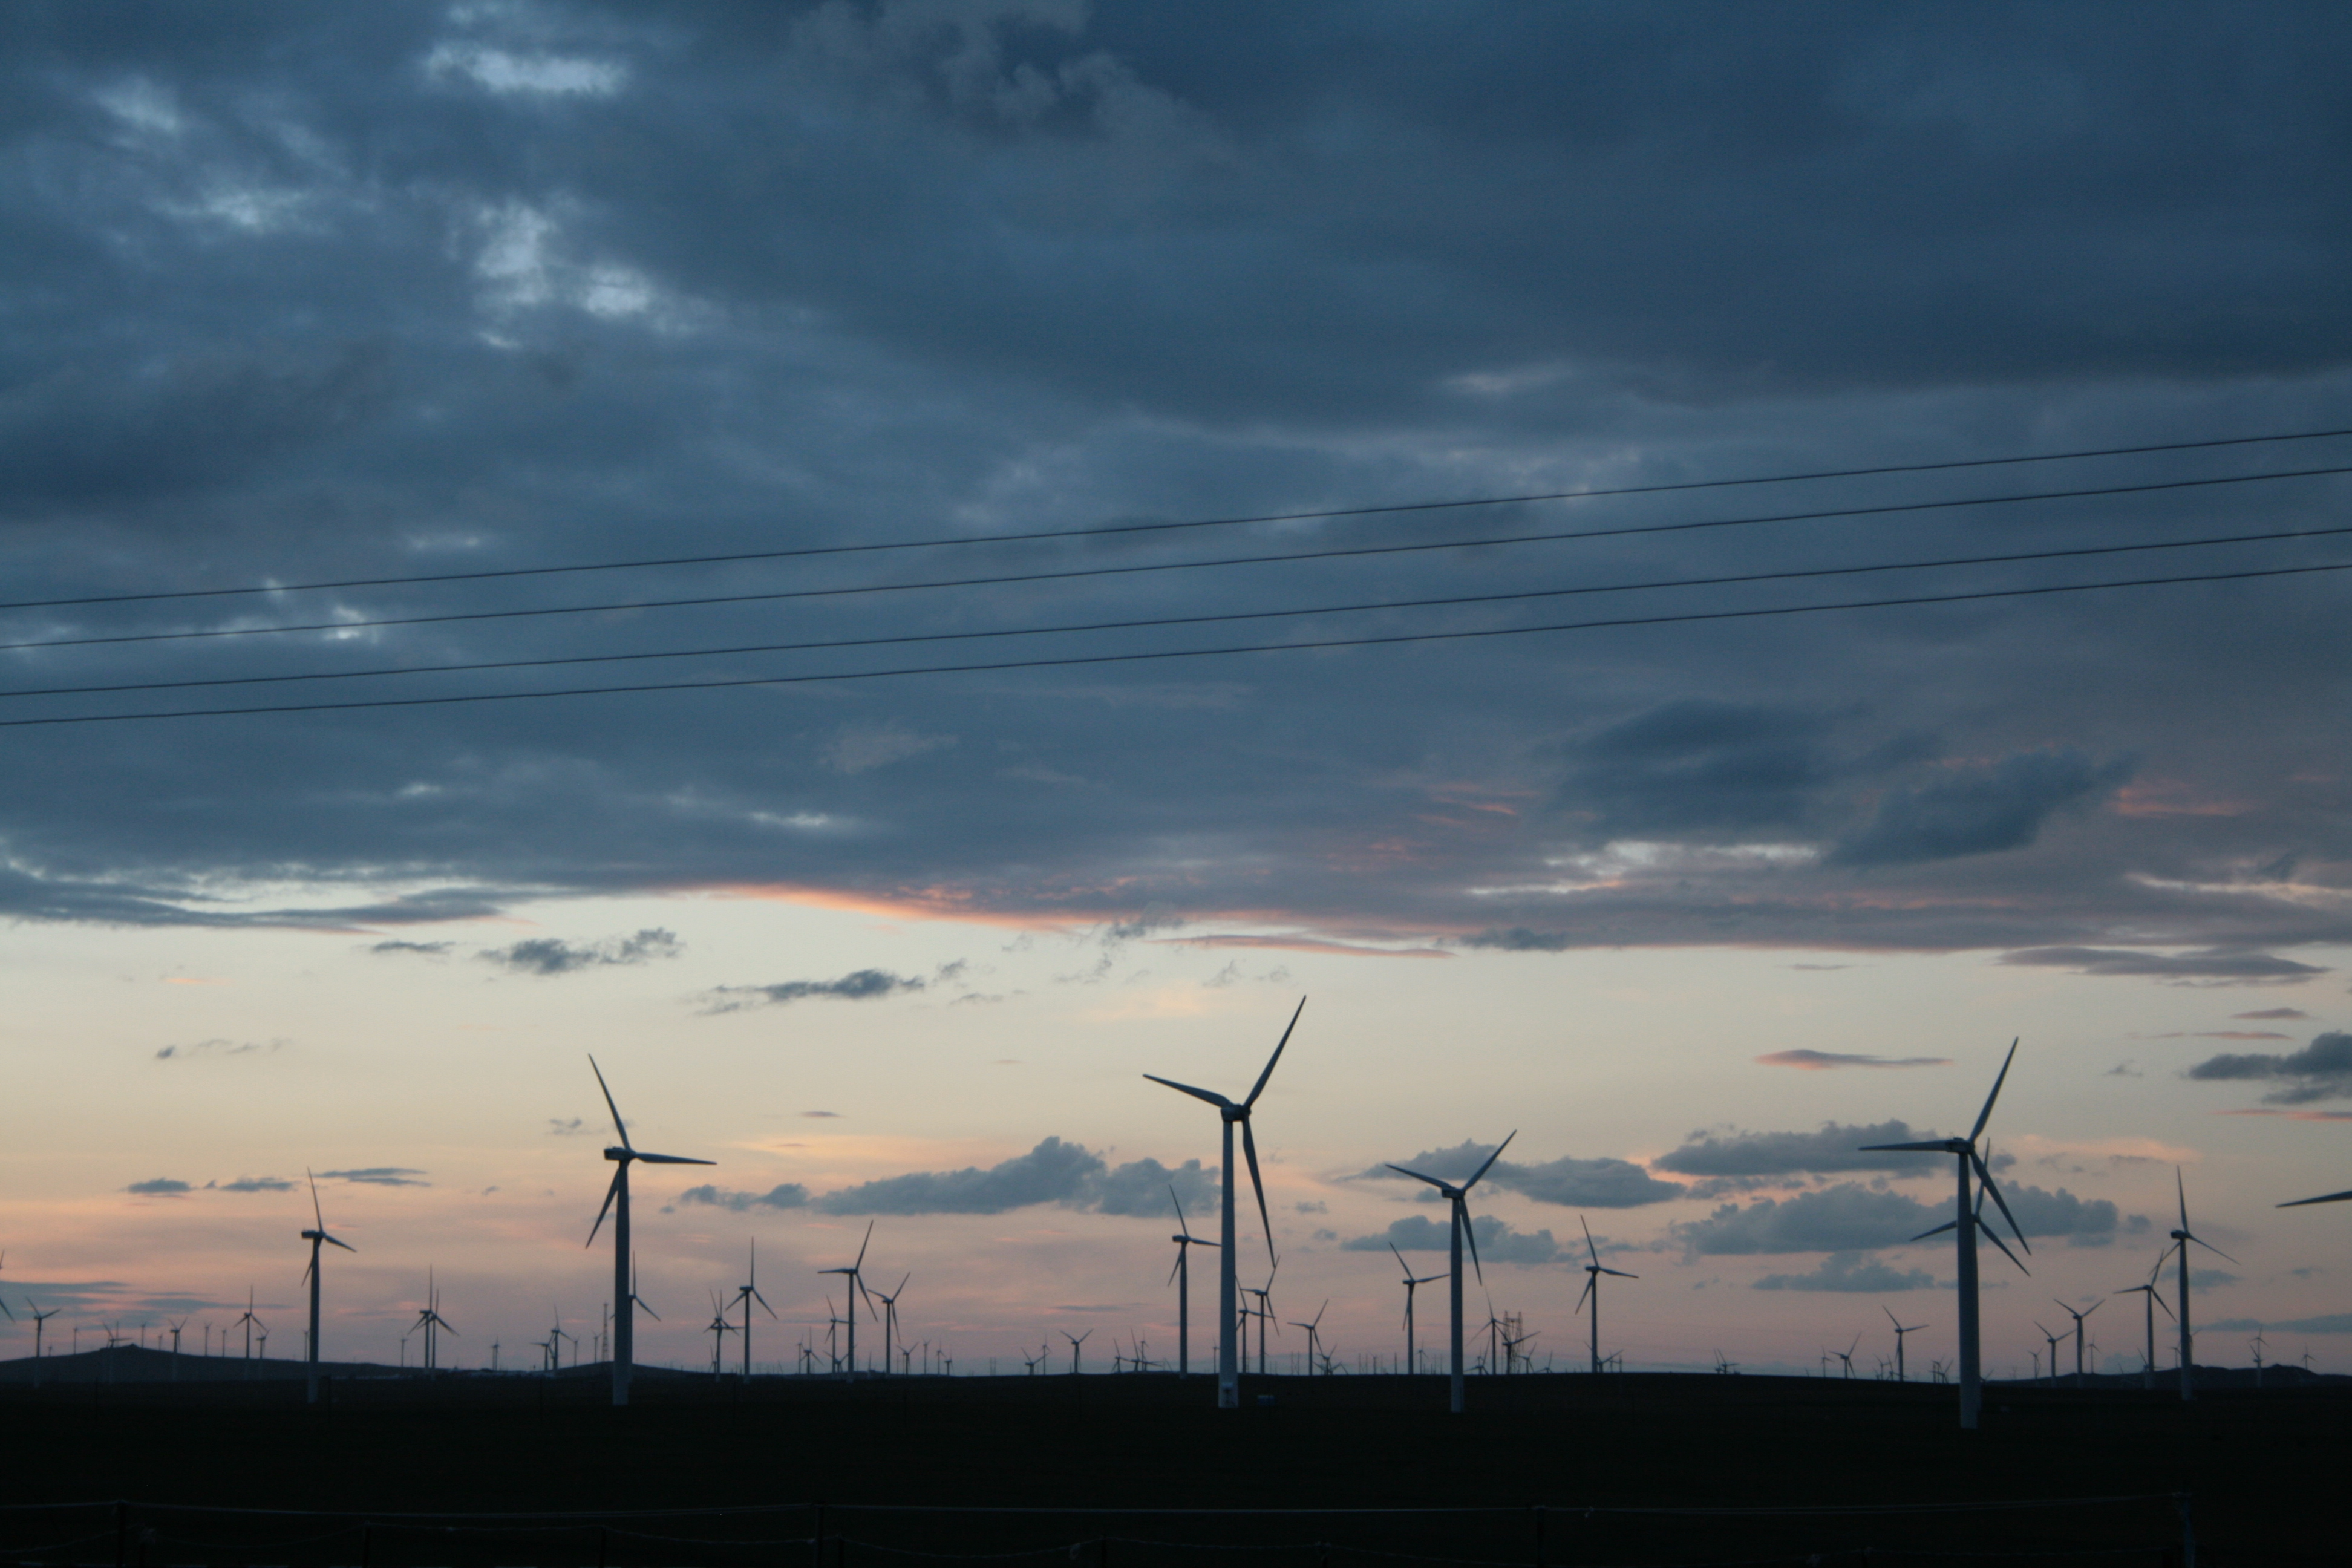
\includegraphics[width=\paperwidth, height=1.1\paperheight]{aeromongolia.JPG}};}
% \begin{frame}{RE in the electricity system}
%   \begin{beamercolorbox}[wd={11cm}, ht={3.2cm},
% sep=3mm,center,rounded=true,
% shadow=false]{postit}
% \begin{itemize}  
%   \item Demand and supply need to be \alert{balanced}.
%   \item Electricity systems are designed for centralized \alert{conventional power plants}.
%   \item \alert{VRE}: variable renewable energy.
%   \end{itemize}
% \end{beamercolorbox}
% \end{frame}
% }

\begin{frame}{RE in the electricity system (supply side)}
\centering\Large {Supply = Demand}
\small{  \begin{itemize}  
%  \item <2->Demand and supply need to be \textbf{\alert{balanced}}.
  \item Electricity systems are designed for centralized \alert{conventional power plants}.
    \begin{itemize}
    \item \textbf{Dispachable} energy
    \end{itemize}
  \item \textbf{\alert{VRE}}: variable renewable energy.
    \begin{itemize}
    \item (most) \textbf{Non-dispachable}
      \begin{itemize}
         \item \textbf{\alert{Intermittency}}: not synchronized with the demand
         \item Need of forecasting, plannification and/or storage
         \item Variations \textbf{from short to long scales} (weather to climate)
  \end{itemize}
  \end{itemize}  
  \end{itemize}}
%\centering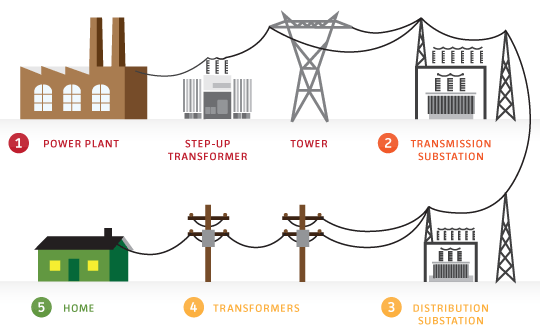
\includegraphics[width=0.5\textwidth]{system.png}
\end{frame}


\begin{frame}{VRE: variable renewable energy}
\vspace{0.1\baselineskip}\centering Variations \textbf{from short to long scales}\\ (weather to climate)\\
\vspace{1\baselineskip}
\begin{columns}
  \begin{column}{0.4\textwidth}
%  \item RE variable in space and time
\small{    \begin{itemize}
    \item \alert{short}: operation
    \item \alert{medium}: planning, maintenance
    \item \alert{long}: resource assessment, financing, planning
  \end{itemize}}    
\end{column}
\begin{column}{0.65\textwidth}
  \centering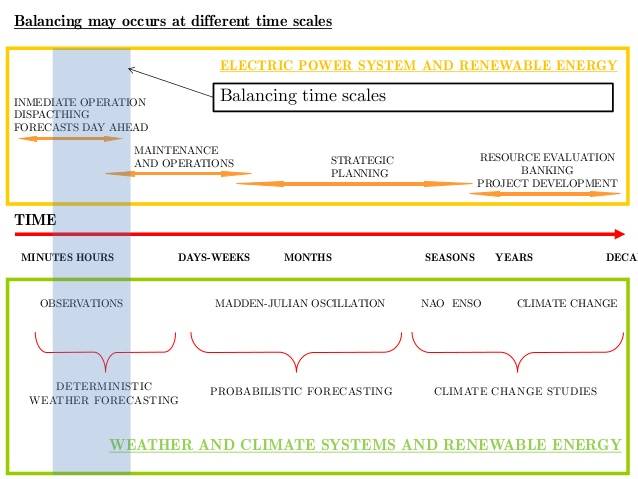
\includegraphics[width=1\textwidth]{timescales.jpg}
\end{column}
\end{columns}
%\centering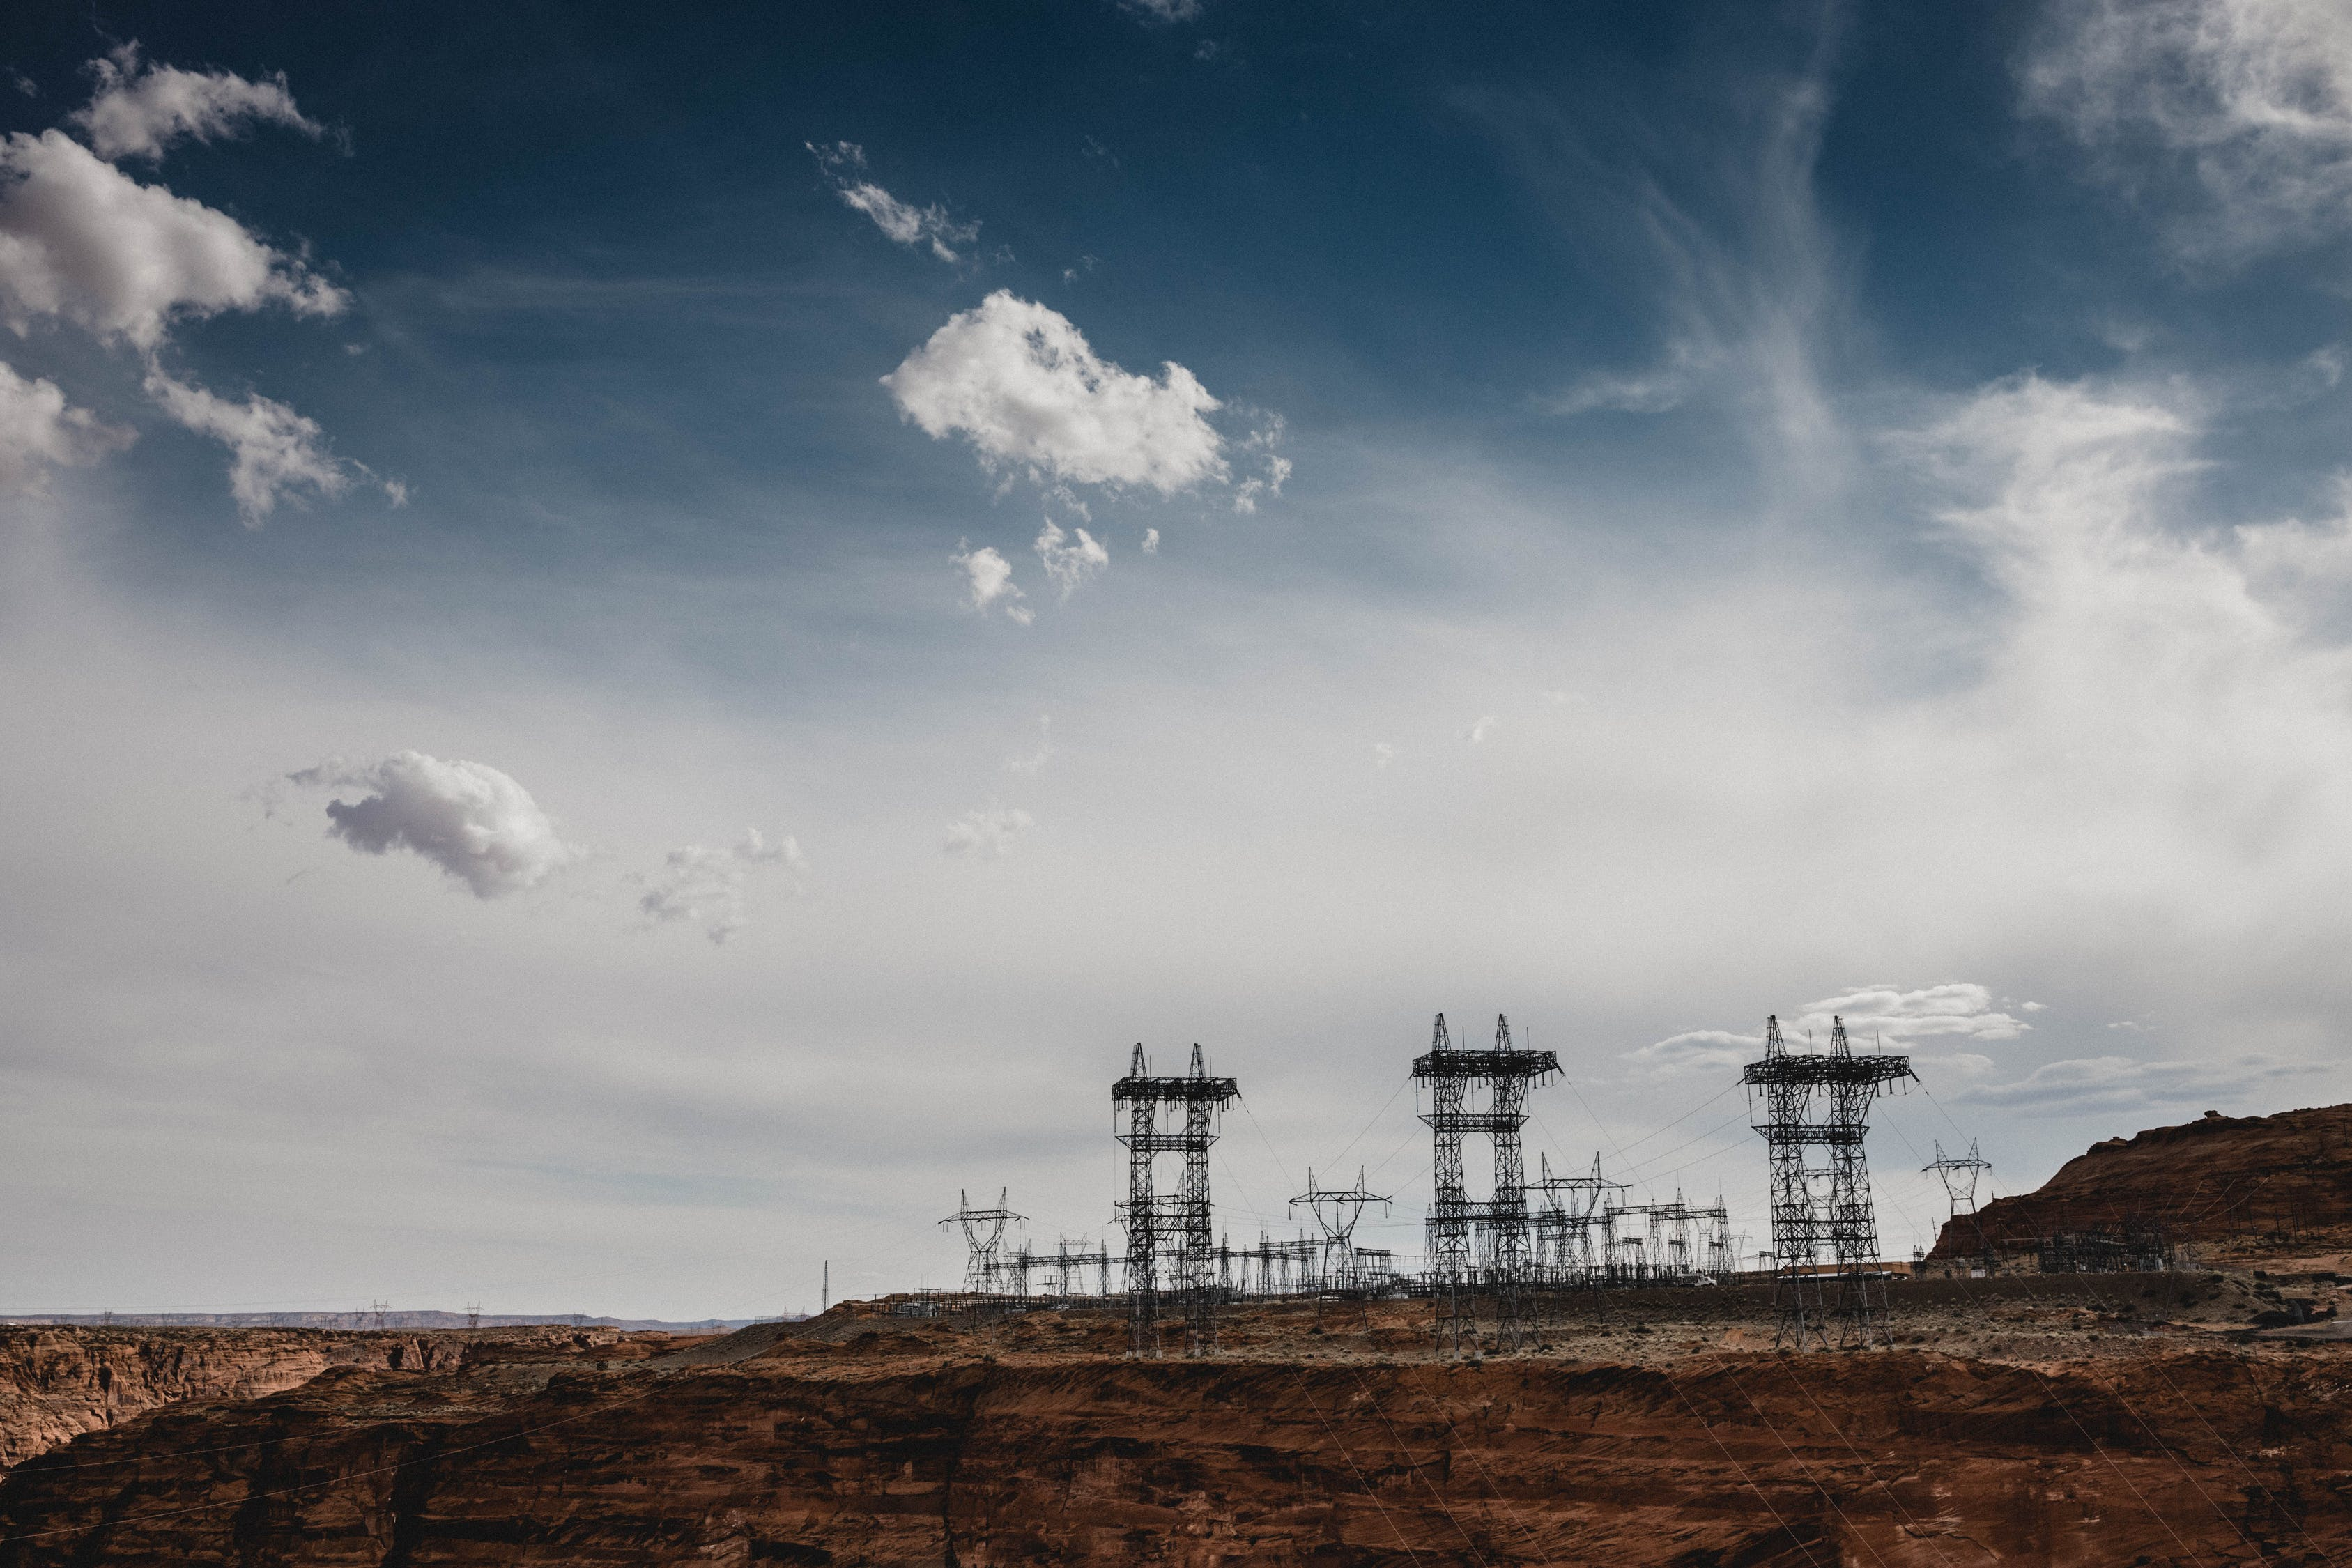
\includegraphics[width=0.5\textwidth]{powerline3.jpeg}
% \end{column}
% \begin{column}{0.3\textwidth}
% \end{column}
% \end{columns}
\end{frame}

% \begin{frame}{Long scales: links between climate and renewables}
% \centering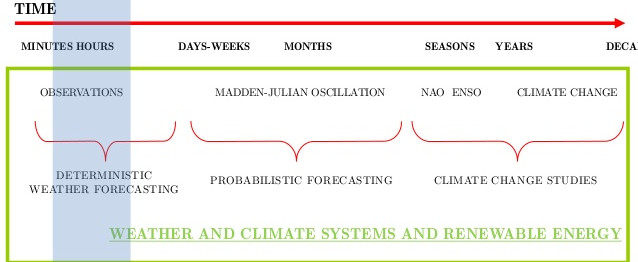
\includegraphics[width=0.8\textwidth]{timescales2.jpg}
% \end{frame}
 

% {
% \usebackgroundtemplate{\tikz\node[opacity=0.5, inner sep=0pt,outer sep=0pt]{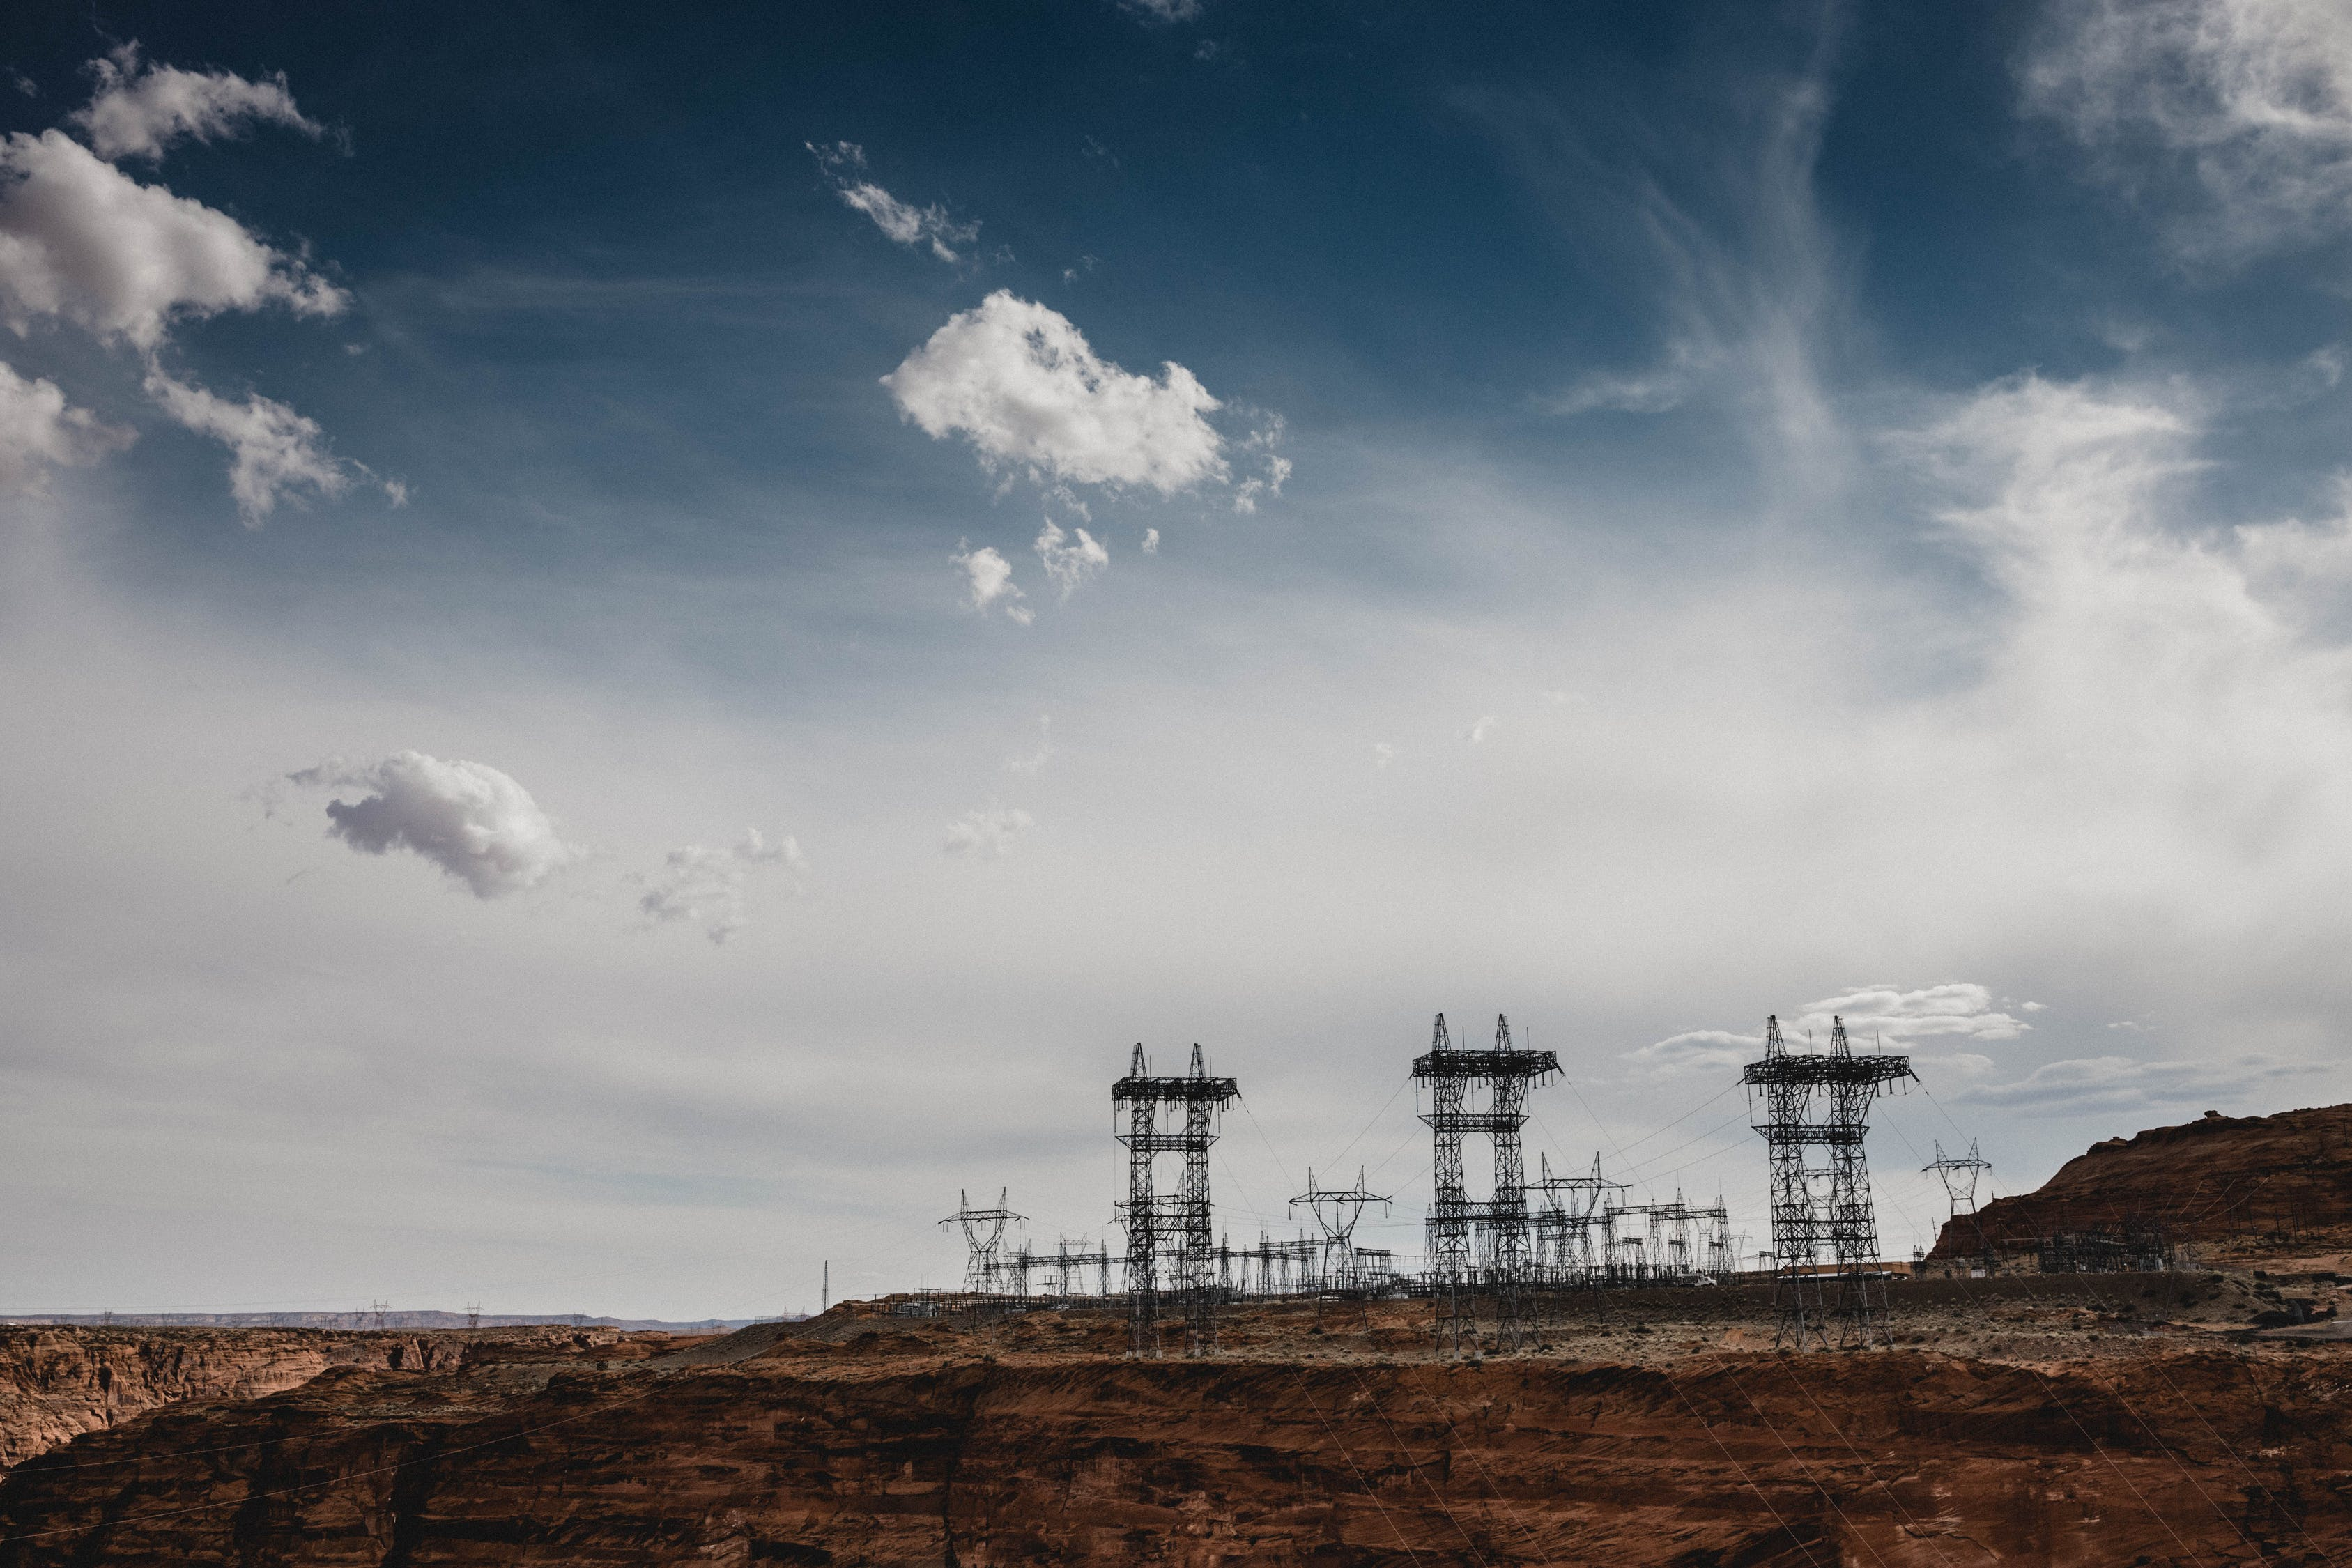
\includegraphics[width=\paperwidth, height=\paperheight]{powerline3.jpeg}};}
% \begin{frame}{VRE}
% \Large{\centering{Need for long-term projections of \textbf{\alert{resource and PV potential}}\\}}
% \vspace{1\baselineskip}
%   \begin{columns}
%    \begin{column}{0.6\textwidth}
%   \begin{itemize}
%   \item RE variable in space and time
%   \item Not syncrinized with the demand
%   \item Need of forecasting, plannification, storage
%   \item Variations from short to long-scales
%     \begin{itemize}
%     \item short: operation
%     \item medium: planning, maintenance
%     \item long: resource assessment, financing, planning
%   \end{itemize}    
%   \end{itemize}
%  \end{column}
%  \begin{column}{0.3\textwidth}
%  \end{column}
%  \end{columns}
% \end{frame}
% }


\begin{frame}[plain]{Variability sources on PV}
  \begin{columns}
    \begin{column}{0.5\textwidth}
  \begin{enumerate}
  \item Astronomical factors  
  \item Atmospheric factors
  \item PV system factors
    \item Other factors
    \end{enumerate}
\end{column}
\begin{column}{0.5\textwidth}    
\end{column}
\end{columns}
\end{frame}


\begin{frame}[plain]{Variability sources on PV}
  \begin{columns}
    \begin{column}{0.5\textwidth}
  \begin{enumerate}
  \item Astronomical factors  
  \item <2->Atmospheric factors
    \begin{itemize}
    \item clouds
    \item aerosols
    \end{itemize}    
  \item <3->PV system factors
    \begin{itemize}
    \item  power plant size
    \item distance between plants
    \end{itemize}
    \item <4->Other factors
      \begin{itemize}
      \item temperature
      \item soiling
      \end{itemize}
  \end{enumerate}
\end{column}
\begin{column}{0.65\textwidth}    
       \begin{figure}
       \begin{figure}
\only<3>{\centering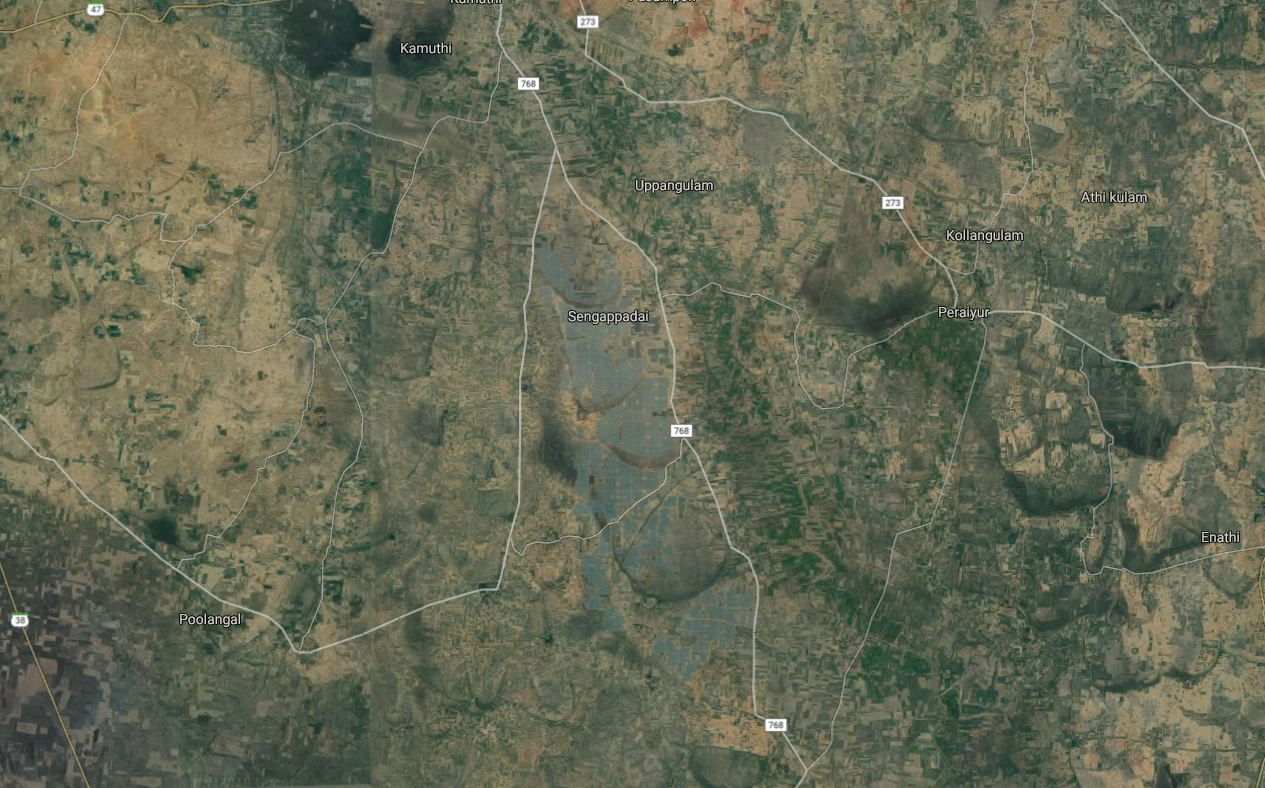
\includegraphics[scale=0.15]{pvplant}
        \centering\caption{Relationship between sun position and the PV generator plane}}
      \end{figure}
       \begin{figure}
\only<4>{\centering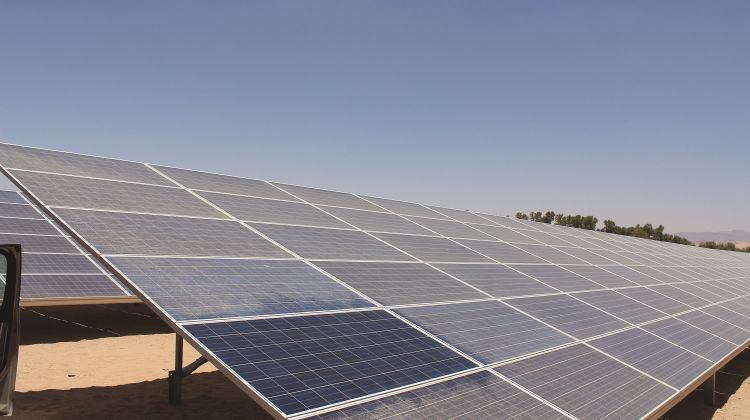
\includegraphics[scale=0.2]{pvmodule}
        \centering\caption{Relationship between sun position and the PV generator plane}}
      \end{figure}
\only<2>{\centering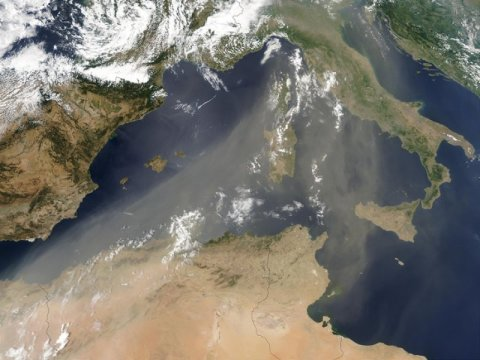
\includegraphics[scale=0.28]{ImageMODIScreditNASA}
        \centering\caption{Relationship between sun position and the PV generator plane}}
      \end{figure}
       \begin{figure}
\only<1>{\centering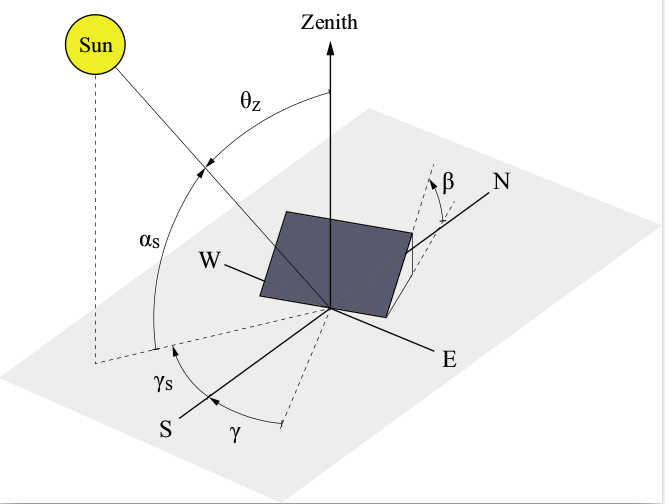
\includegraphics[scale=0.28]{astronomical}
        \centering\caption{Relationship between sun position and the PV generator plane}}
      \end{figure}
    \end{column}
  \end{columns}
\end{frame}

%|\only<2>{\includegraphics{fig}}|
%|\uncover<2>{\includegraphics{fig}}|
%|\visible<2>{\includegraphics{fig}}|

\begin{frame}[fragile]{MOTIVATION}
\Large{\centering{\textbf{Broaden knowledge on spatiotemporal behaviour of solar resource and \alert{PV production} over the Med\\}}}
\vspace{1\baselineskip}
\small{\begin{itemize}
     \item \alert{Time scale:} Often neglected time scale: climate perspective.
     \item \alert{Variability factors:} Often neglected impact of aerosols.
     \item Availability (or potential changes) of solar resource under \alert{climate change} scenarios.  
     \end{itemize}}
\end{frame}

\section{Objectives and methods}

\begin{frame}[fragile]{GENERAL OBJECTIVES}
\centering{\textbf{Approaches to different scientific questions}}
\vspace{1\baselineskip}
\small{\begin{itemize}
  \item[]<2-> {\Huge{\alert{1}}} To systematize the spatiotemporal analysis of solar resource and photovoltaic productio \through a comprhensive method.
    \begin{itemize}
    \item<3-> To charactericed \textbf{interannual} variability of solar resource and photovoltaic productivity over the Iberian Peninsula.
      \end{itemize}
%    \vspace{1.5\baselineskip}
    \item[]<4-> {\Huge{\alert{2}}} To quantify the impact of \textbf{aerosols} on the spatiotemporal variability of PV productivity over the Euro-Mediterranean area.
      \begin{itemize}
      \item <5->Investigate the RCMs added values in resource assessment studies.
        \end{itemize}
  \item[]<6-> {\Huge{\alert{3}}} To analyze \textbf{future projections} of photovoltaic potential and the role of aerosols.
  \end{itemize}}
\end{frame}

\begin{frame}[fragile]{METHODS: modelization of PV productivity}
\vspace{0\baselineskip}
\textbf{\alert{PV productivity}}\\
\vspace{1\baselineskip}
{\centering{\Large\textbf{{Solar radiation + PV system}}}}
\vspace{1\baselineskip}
\begin{columns}
  \begin{column}{0.4\textwidth}
    \small{    \begin{blockalert}\begin{itemize}
    \item From \textbf{measurements}
% \begin{tikzpicture}[remember picture,overlay]
% \node[draw,line width=1pt,cyan, circle,inner ysep=50pt,fit={(pic cs:start) (pic cs:end)}] {};
% \end{tikzpicture} 
    \item From \textbf{satellite}
    \item From \textbf{RCMs}  
      \end{itemize}\end{blockalert}}
  \end{column}
  \begin{column}{0.6\textwidth}
% \begin{tikzpicture}[overlay, remember picture]
% \node[draw,line width=1pt,cyan, circle,inner ysep=50pt,fit={(pic cs:start) (pic cs:end)}] {};
% \end{tikzpicture}
    \begin{figure}
      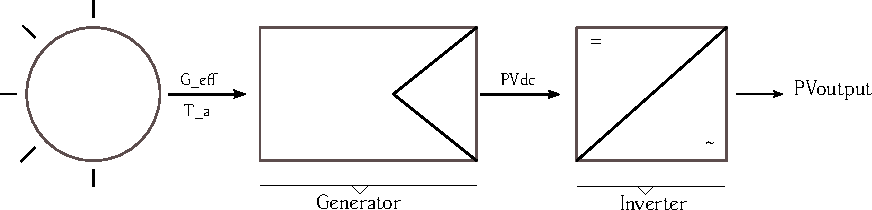
\includegraphics[scale=0.45]{pvsistem.pdf}
      \centering\caption{Squeme of a PV generator.}
    \end{figure}
  \end{column}
\end{columns}
\end{frame}

\section{Results. Part I}

\subsection{Multi-step scheme and spatial analysis of long-term characteristics of photovoltaic productivity over the Iberian Peninsula}

\begin{frame}[standout]
\centering{Multi-step scheme and spatial analysis of long-term characteristics of photovoltaic productivity over the Iberian Peninsula\footnote{\tiny{\textcolor{white}{This chapter has been published as a paper in Solar Energy journal; doi:}}}}
\end{frame}

\begin{frame}[fragile]{Introduction}
\only<1->{Natural variability of renewable energy resources comes from short to longer scales. A \textbf{comprehensive} analysis should include \textbf{\alert{spatial}} and \textbf{\alert{temporal}} characteristics.\\}
\vspace{1\baselineskip}
\only<2-> {\textbf{Spatial} characteristics can be analysed by \alert{regionalization}\footnote{It attempts to capture the spatial variability of climate} approaches.\\}
\vspace{1\baselineskip}
\only<3->{\textbf{\alert{Clustering}} methods: \textbf{objective} methodology
  \begin{itemize}
  \item Used for some climate variables.
  \item Used for short-term analysis in solar resource.
  \end{itemize}}  
\end{frame}

\begin{frame}[fragile]{Introduction}
The \textbf{\alert{interannual}} variability affects renewable energy projects:   
  \begin{itemize}
  \item It impacts on the project yearly production, \textbf{yearly revenues}, and project \textbf{financing}.
  \end{itemize}
However, it has been sometimes \textbf{\alert{discounted}} [Bryce 2018].
  \begin{itemize}
  \item Use of \textbf{TMY} datasets (not enough).
  \end{itemize}
Year-to-year \textbf{\alert{monthly series}} (of solar resource) are highly \textbf{variable} due to large-scale circulation modes.   
\end{frame}


\begin{frame}[fragile]{Objective}
To \textbf{\alert{systematize}} the \textbf{\alert{spatiotemporal analysis}} of solar resource and photovoltaic production through a comprhensive method:
  \begin{enumerate}
  \item Obtain a \textbf{regionalization}
  \item Analyse \textbf{variability} (PV, resource)
  \item Analyse \textbf{complementarity}
  \end{enumerate}
\end{frame}


% \begin{frame}[fragile]{Data}
%   Use of satellite dataset from \textbf{CM-SAF}:
%   \begin{itemize}
%   \item SARAH dataset
%   \item horizontal resolution: $0.05ºx 0.05º$
%   \item time resolution: daily
%   \end{itemize}   
% \end{frame}
 
\begin{frame}[fragile]{Method}
\begin{figure}  
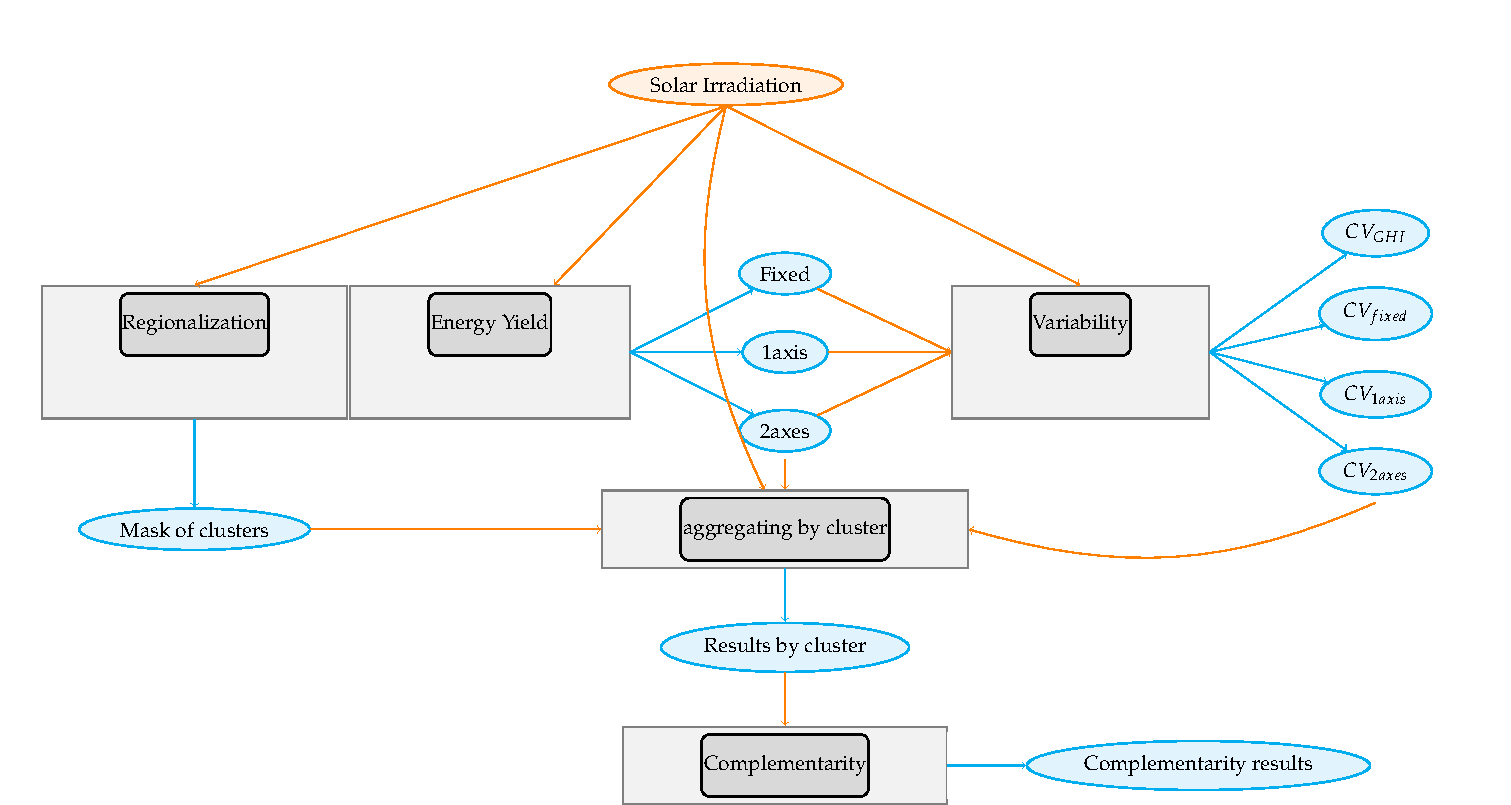
\includegraphics[scale=0.45]{multi_step.pdf}
\end{figure}
\end{frame}

\begin{frame}[fragile]{Method}
\begin{figure}  
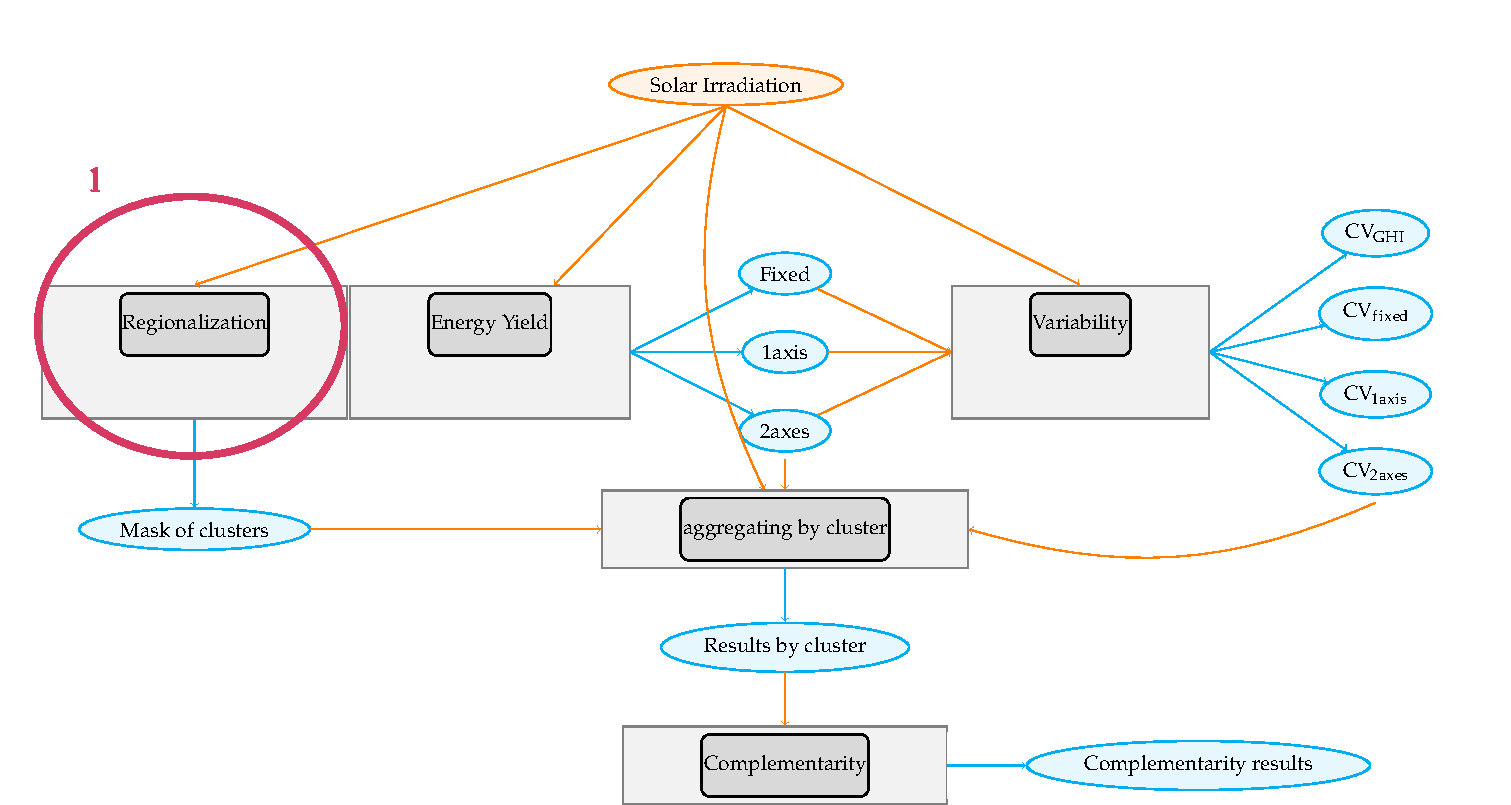
\includegraphics[scale=0.45]{multi_step1.pdf}
\end{figure}
\end{frame}

\begin{frame}[fragile]{Method: regionalization}
  \begin{itemize}
  \item[] <1-> Obtain a regionalization: \textbf{\alert{clustering}} algorithms
  \begin{itemize}
  \item \textbf{PCA}: principal component analysis
    \begin{itemize}
    \item {\tiny{To reduce dimensionality}}
    \end{itemize}  
  \item \textbf{hierarchical + k-means}
    \begin{itemize}
    \item {\tiny{To obtain an optimal partition} through an optimization or objective function.}
    \end{itemize}  
  \item validation: CH index + ``L-method''
  \end{itemize}   
% \item[] <2-> Analyse variability: \textbf{\alert{coefficient of variability}}
%   \begin{equation} \small{CV=\frac{\sigma}{\bar{X}}}
%   \end{equation}  
%   \item[] <3-> Analyse complementarity: \textbf{\alert{correlation}} between clusters
%     \begin{itemize}
%     \item 15-year moving window.
%       \end{itemize}
  \end{itemize}
\end{frame}

\begin{frame}[fragile]{Method}
\begin{figure}  
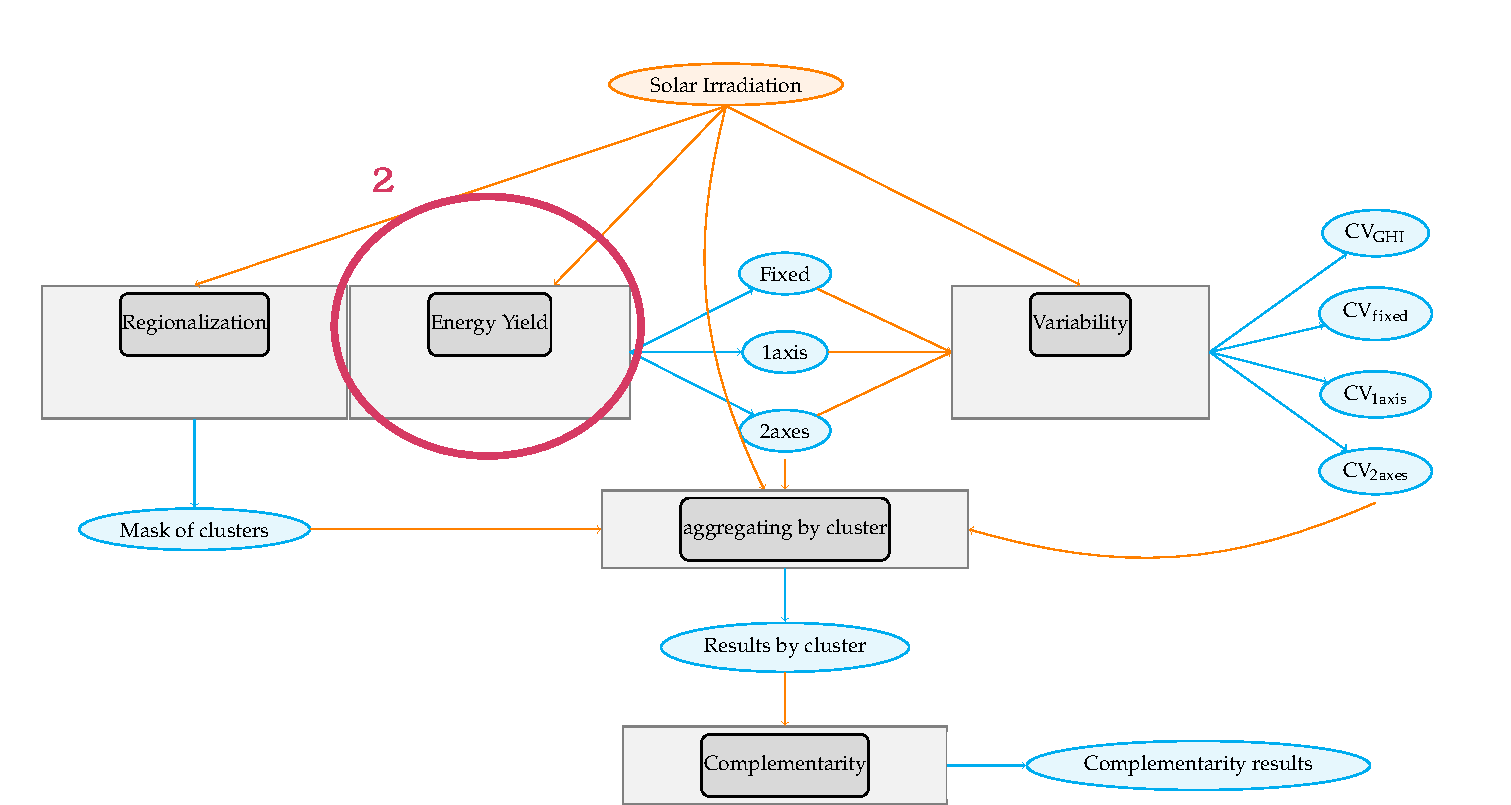
\includegraphics[scale=0.45]{multi_step2.pdf}
\end{figure}
\end{frame}

\begin{frame}[fragile]{Method}
\begin{figure}  
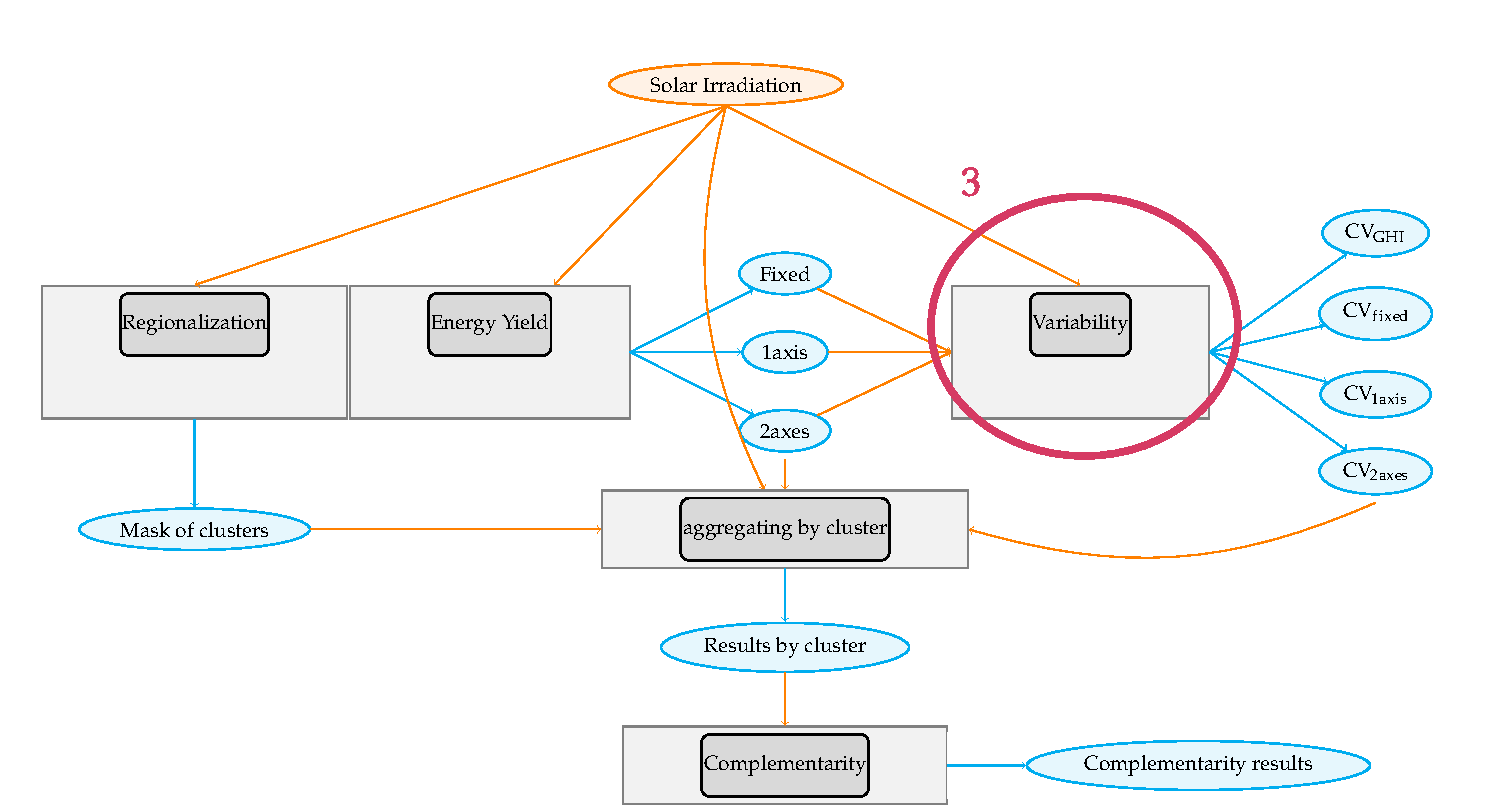
\includegraphics[scale=0.45]{multi_step4.pdf}
\end{figure}
\end{frame}

\begin{frame}[fragile]{Method}
   \begin{itemize}
  % \item[] <1-> Obtain a regionalization: \textbf{\alert{clustering}} algorithms
  % \begin{itemize}
  % \item \textbf{PCA}: principal component analysis
  %   \begin{itemize}
  %   \item {\tiny{To reduce dimensionality}}
  %   \end{itemize}  
  % \item \textbf{hierarchical + k-means}
  %   \begin{itemize}
  %   \item {\tiny{To obtain an optimal partition} through an optimization or objective function.}
  %   \end{itemize}  
  % \item validation: CH index + ``L-method''
  % \end{itemize}   
\item[] Analyse variability: \textbf{\alert{coefficient of variability}}
  \begin{equation} \small{CV=\frac{\sigma}{\bar{X}}}
  \end{equation}  
  % \item[] <3-> Analyse complementarity: \textbf{\alert{correlation}} between clusters
     \begin{itemize}
     \item Interannual variability of yearly values
     \item Monthly series  
     \end{itemize}
\end{itemize}
\end{frame}

\begin{frame}[fragile]{Method}
\begin{figure}  
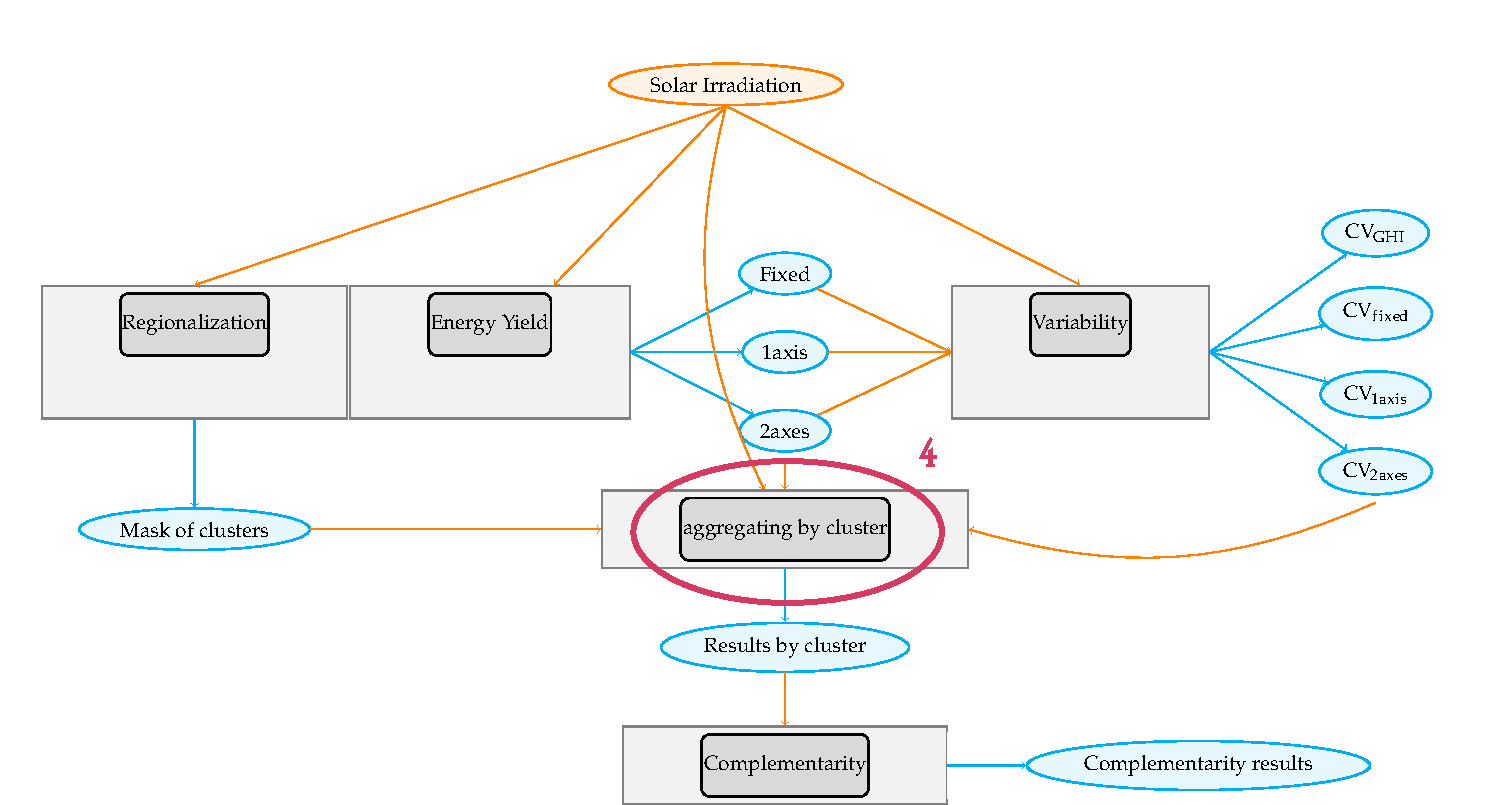
\includegraphics[scale=0.45]{multi_step5.pdf}
\end{figure}
\end{frame}

\begin{frame}[fragile]{Method}
\begin{figure}  
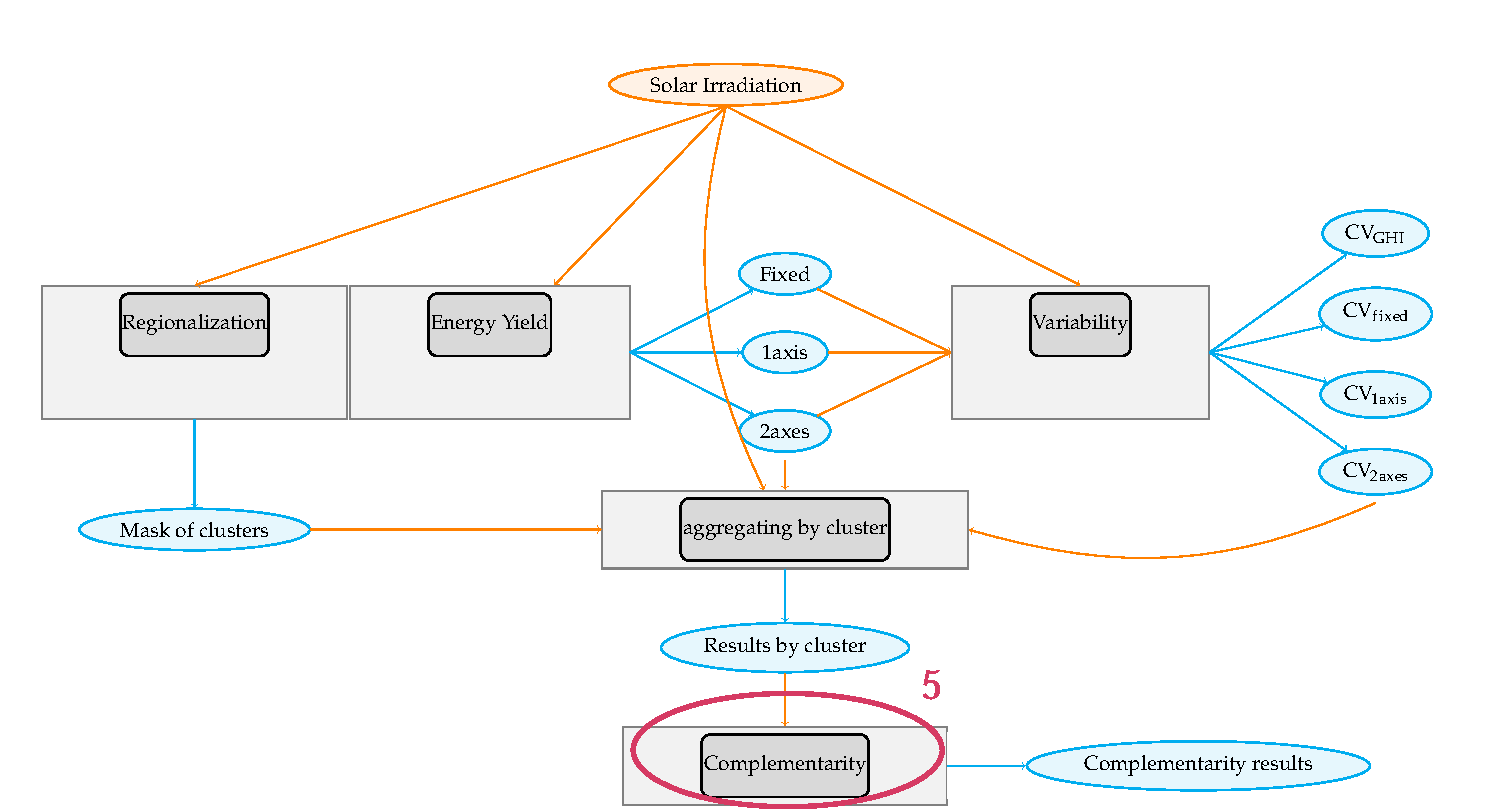
\includegraphics[scale=0.45]{multi_step6.pdf}
\end{figure}
\end{frame}

\begin{frame}[fragile]{Method}
   \begin{itemize}
  % \item[] <1-> Obtain a regionalization: \textbf{\alert{clustering}} algorithms
  % \begin{itemize}
  % \item \textbf{PCA}: principal component analysis
  %   \begin{itemize}
  %   \item {\tiny{To reduce dimensionality}}
  %   \end{itemize}  
  % \item \textbf{hierarchical + k-means}
  %   \begin{itemize}
  %   \item {\tiny{To obtain an optimal partition} through an optimization or objective function.}
  %   \end{itemize}  
  % \item validation: CH index + ``L-method''
  % \end{itemize}   
% \item[] Analyse variability: \textbf{\alert{coefficient of variability}}
%   \begin{equation} \small{CV=\frac{\sigma}{\bar{X}}}
%   \end{equation}  
    \item[] Analyse complementarity: \textbf{\alert{correlation}} between clusters
     \begin{itemize}
     \item 15-year moving window.
     \end{itemize}
\end{itemize}
\end{frame}

% \begin{frame}[fragile]{Method}
%   \begin{itemize}
%   \item[] <1-> Obtain a regionalization: \textbf{\alert{clustering}} algorithms
%   \begin{itemize}
%   \item \textbf{PCA}: principal component analysis
%     \begin{itemize}
%     \item {\tiny{To reduce dimensionality}}
%     \end{itemize}  
%   \item \textbf{hierarchical + k-means}
%     \begin{itemize}
%     \item {\tiny{To obtain an optimal partition} through an optimization or objective function.}
%     \end{itemize}  
%   \item validation: CH index + ``L-method''
%   \end{itemize}   
% \item[] <2-> Analyse variability: \textbf{\alert{coefficient of variability}}
%   \begin{equation} \small{CV=\frac{\sigma}{\bar{X}}}
%   \end{equation}  
%   \item[] <3-> Analyse complementarity: \textbf{\alert{correlation}} between clusters
%     \begin{itemize}
%     \item 15-year moving window.
%       \end{itemize}
%   \end{itemize}
% \end{frame}

\begin{frame}[fragile]{Results: application to the IP}
  The \textbf{\alert{IP}} is limited area with high variety of \textbf{climates}. It is also nearly \textbf{isolated} from the electrical point of view.
%  \vspace{\baselineskip}
  \begin{columns}
    \begin{column}{0.5\textwidth}
  \textbf{DATA}:    
  Use of satellite dataset from \textbf{\alert{CM-SAF}}:
  \begin{itemize}
  \item SARAH dataset
  \item horizontal resolution: $0.05ºx 0.05º$
  \item 30 years of daily data
  \end{itemize}   
    \end{column}
    \begin{column}{0.5\textwidth}
      \begin{figure}
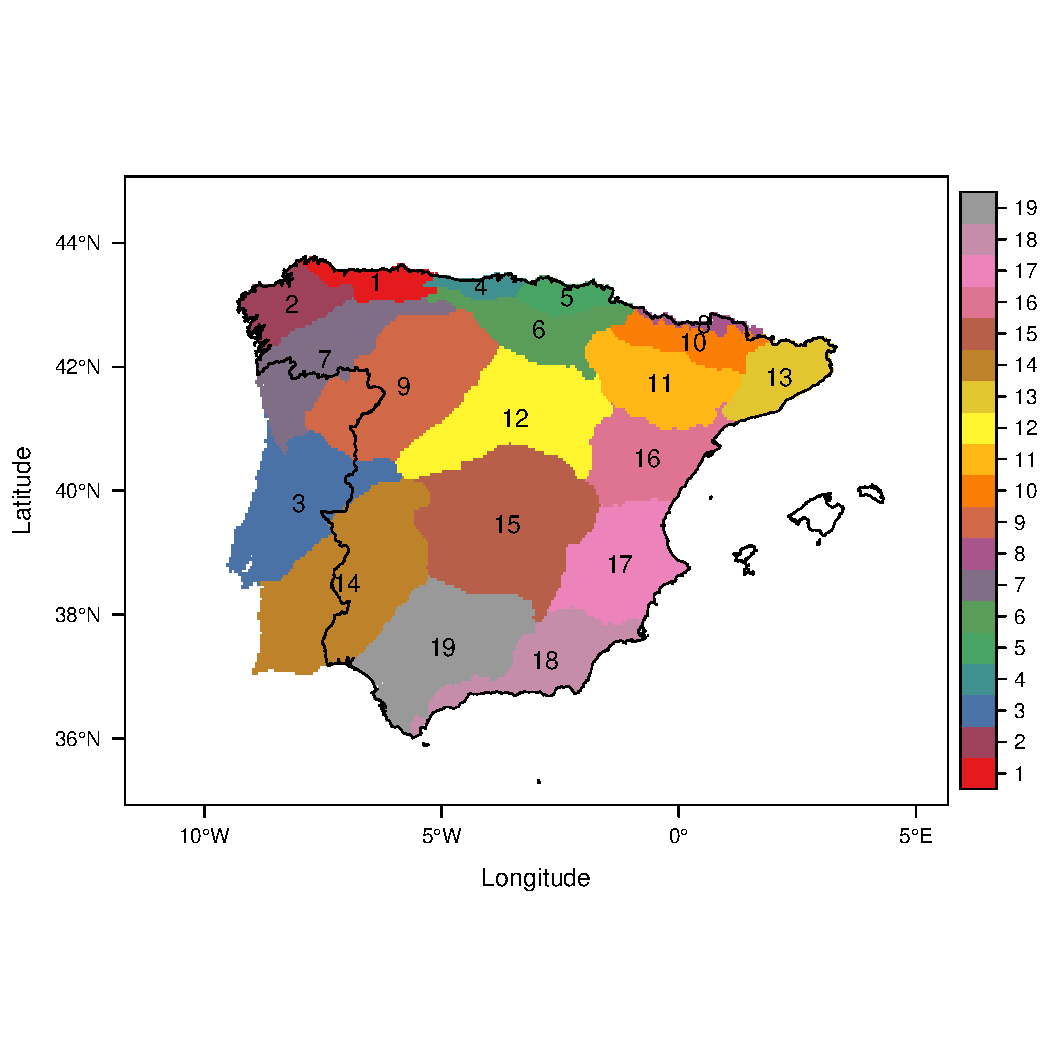
\includegraphics[scale=0.3]{clusters2.pdf}
      \end{figure}
    \end{column}
  \end{columns}
\end{frame}

% \begin{frame}[fragile]{Results: regionalization}
%   \begin{columns}
%     \begin{column}{0.5\textwidth}
%   \textbf{Regionalization}:    
%   \begin{enumerate}
%   \item PCA
%     \begin{itemize}
%     \item {\tiny{To reduce dimensionality}}
%     \end{itemize}  
%   \item \textbf{hierarchical + k-means}
%     \begin{itemize}
%     \item {\tiny{To obtain an optimal partition}}
%     \end{itemize}  
%   \item validation: CH index
%   \end{enumerate}   
%     \end{column}
%     \begin{column}{0.5\textwidth}
%       \begin{figure}
%         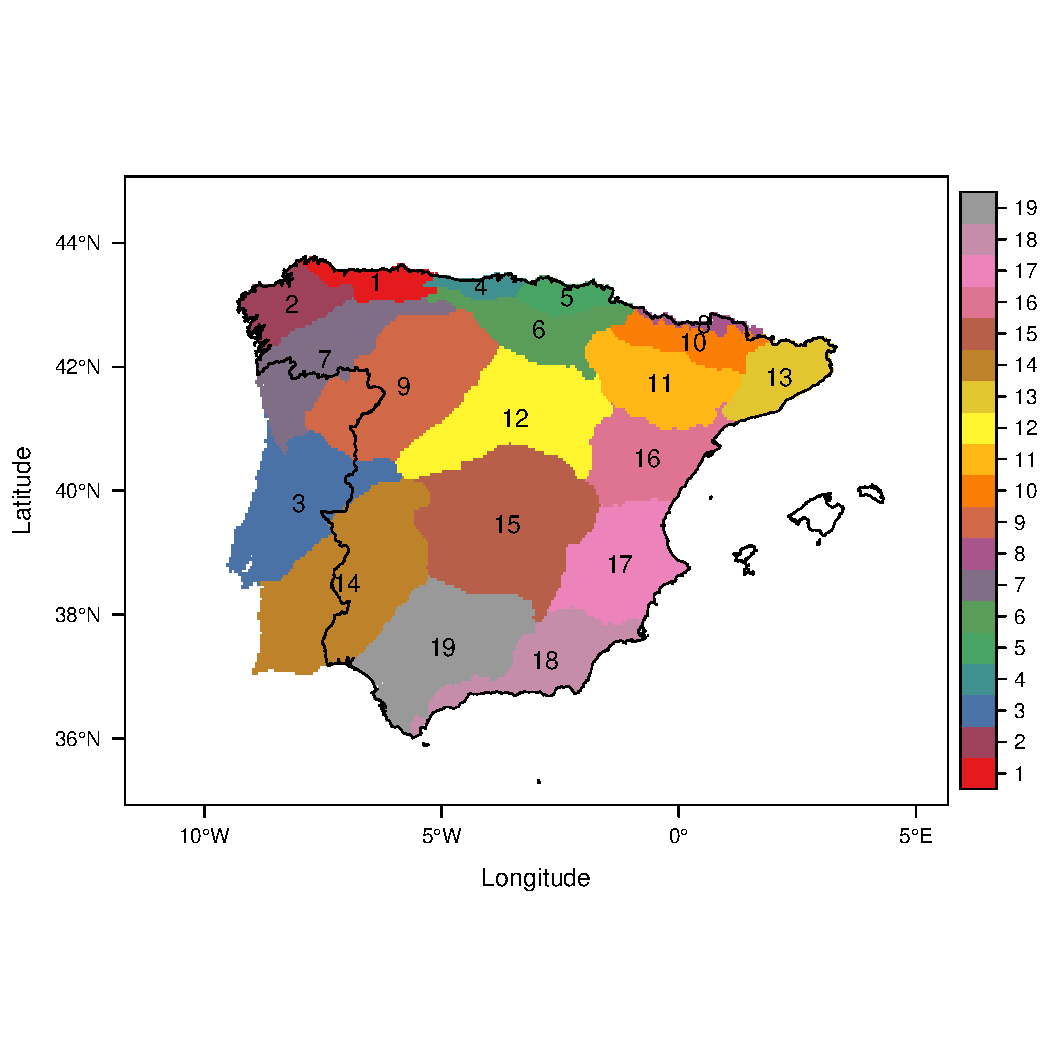
\includegraphics[scale=0.3]{clusters2.pdf}
%       \end{figure}
%     \end{column}
%   \end{columns}
% \end{frame}

\begin{frame}[fragile]{Results: productivity by cluster}
  \begin{columns}
    \begin{column}{0.5\textwidth}
      \begin{figure}
        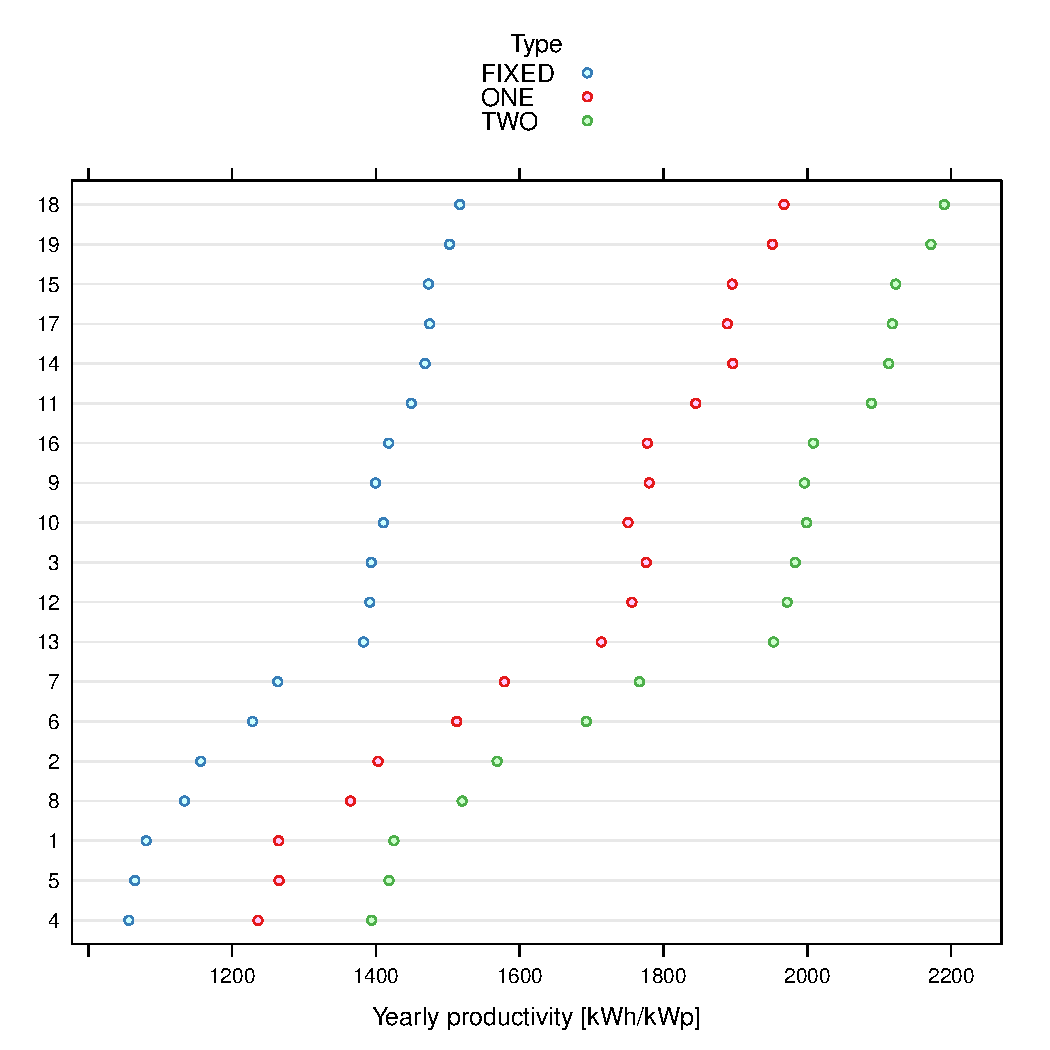
\includegraphics[scale=0.35]{productivity_bycluster_andtype.pdf}
      \end{figure}
    \end{column}
\begin{column}{0.5\textwidth}
\vspace{1.5\baselineskip}  
 \begin{itemize}
 \item <1,2> \textbf{Lower productivity} for lower irradiation values: \textbf{northern clusters.}
 \item <2> Yield increase from fixed to tracking is \alert{non-linear}.
  \end{itemize}  
   \end{column}
  \end{columns}
\end{frame}

\begin{frame}[fragile]{Results: productivity by cluster}
  \begin{columns}
    \begin{column}{0.5\textwidth}
      \begin{figure}
        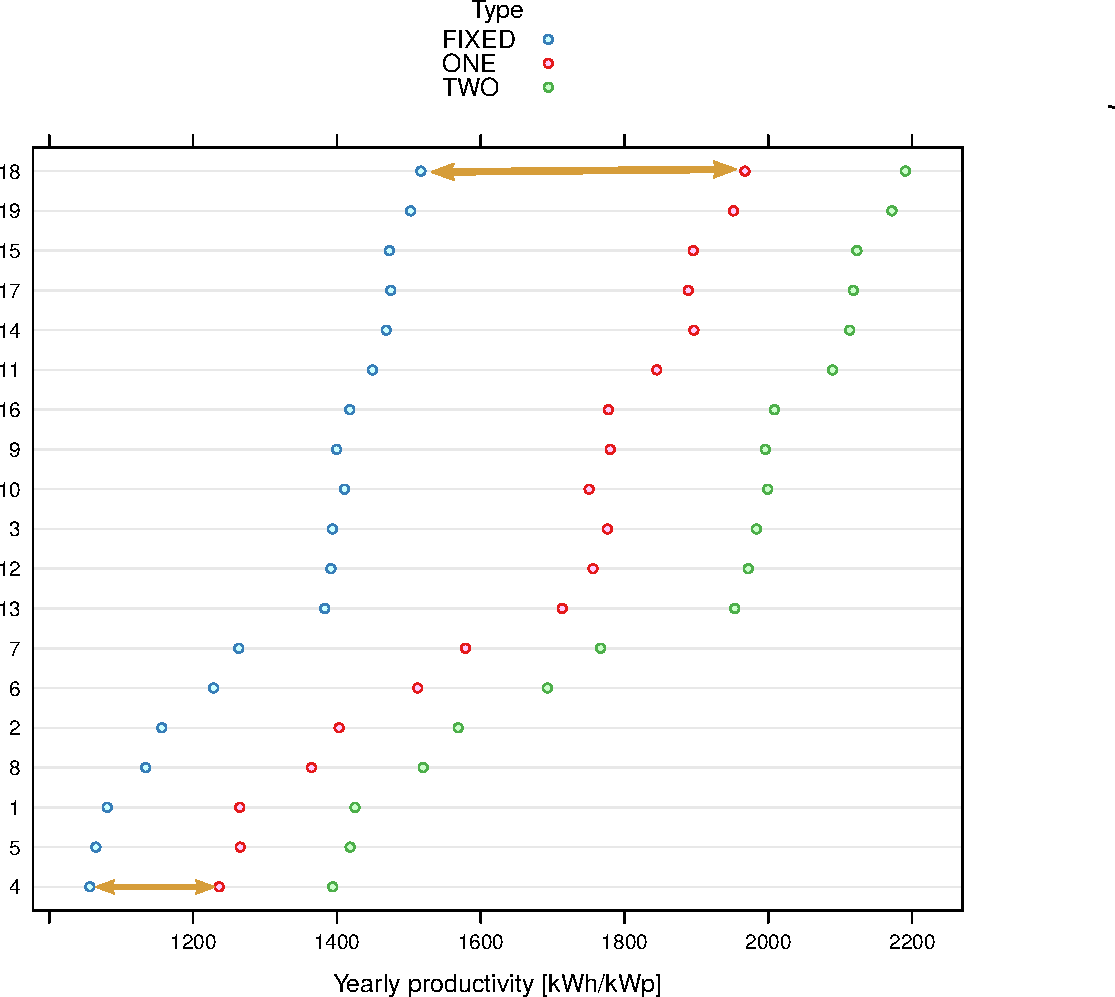
\includegraphics[scale=0.35]{productivity_bycluster_andtype2.pdf}
      \end{figure}
\end{column}
\begin{column}{0.5\textwidth}
\vspace{1.5\baselineskip}  
 \begin{itemize}
 \item \textbf{Lower productivity} for lower irradiation values: \textbf{northern clusters}.
  \item Yield increase from fixed to tracking is \alert{non-linear}. 
  \item Yield \textbf{differences} among clusters is \textbf{higher} for \textbf{\alert{tracking systems}}.
  \end{itemize}  
   \end{column}
  \end{columns}
\end{frame}

\begin{frame}[fragile]{Results: variability}
  \begin{columns}
    \begin{column}{0.6\textwidth}
      \begin{figure}
        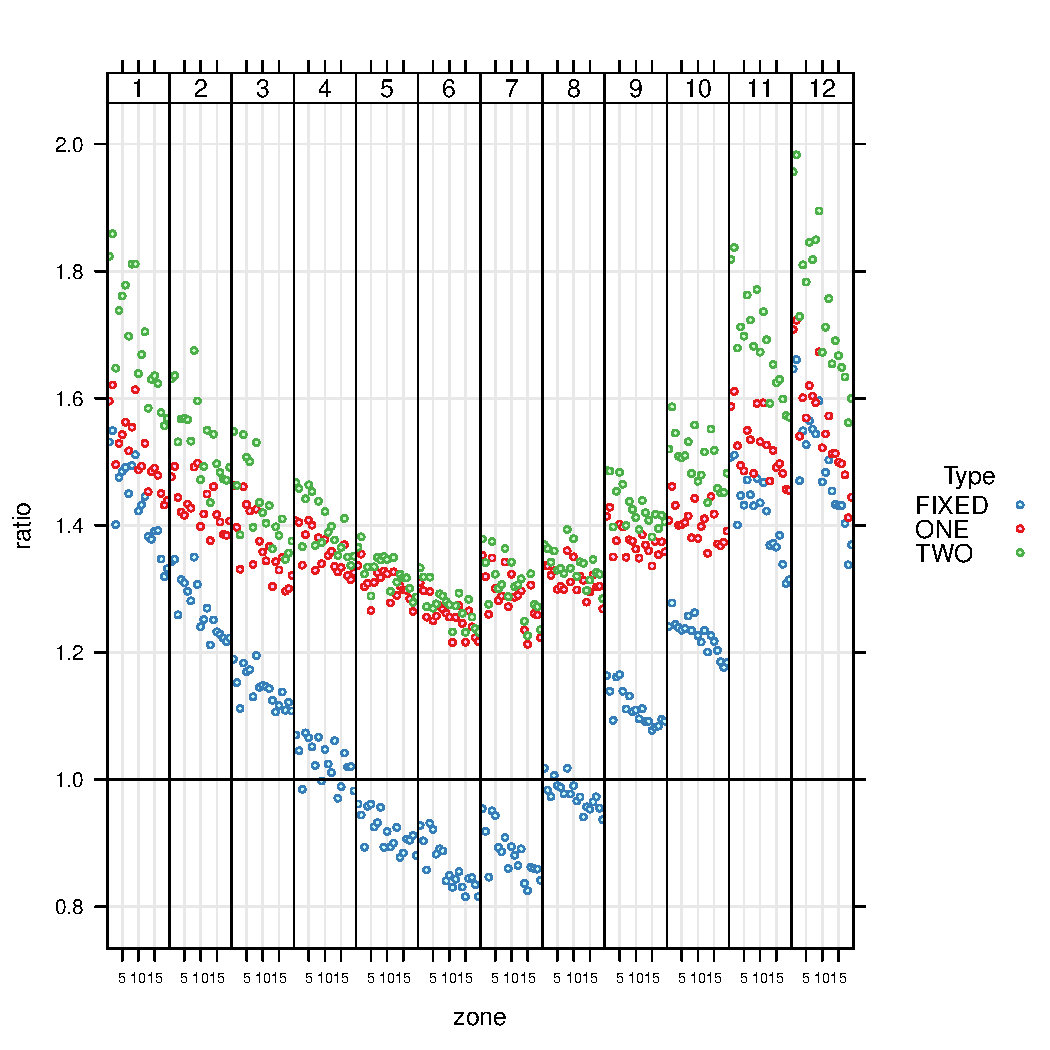
\includegraphics[scale=0.4]{dotplot_ratio_zone2.pdf}
      \end{figure}
\end{column}
    \begin{column}{0.5\textwidth}
%       \begin{figure}
% \hspace{1.5\baselineskip}{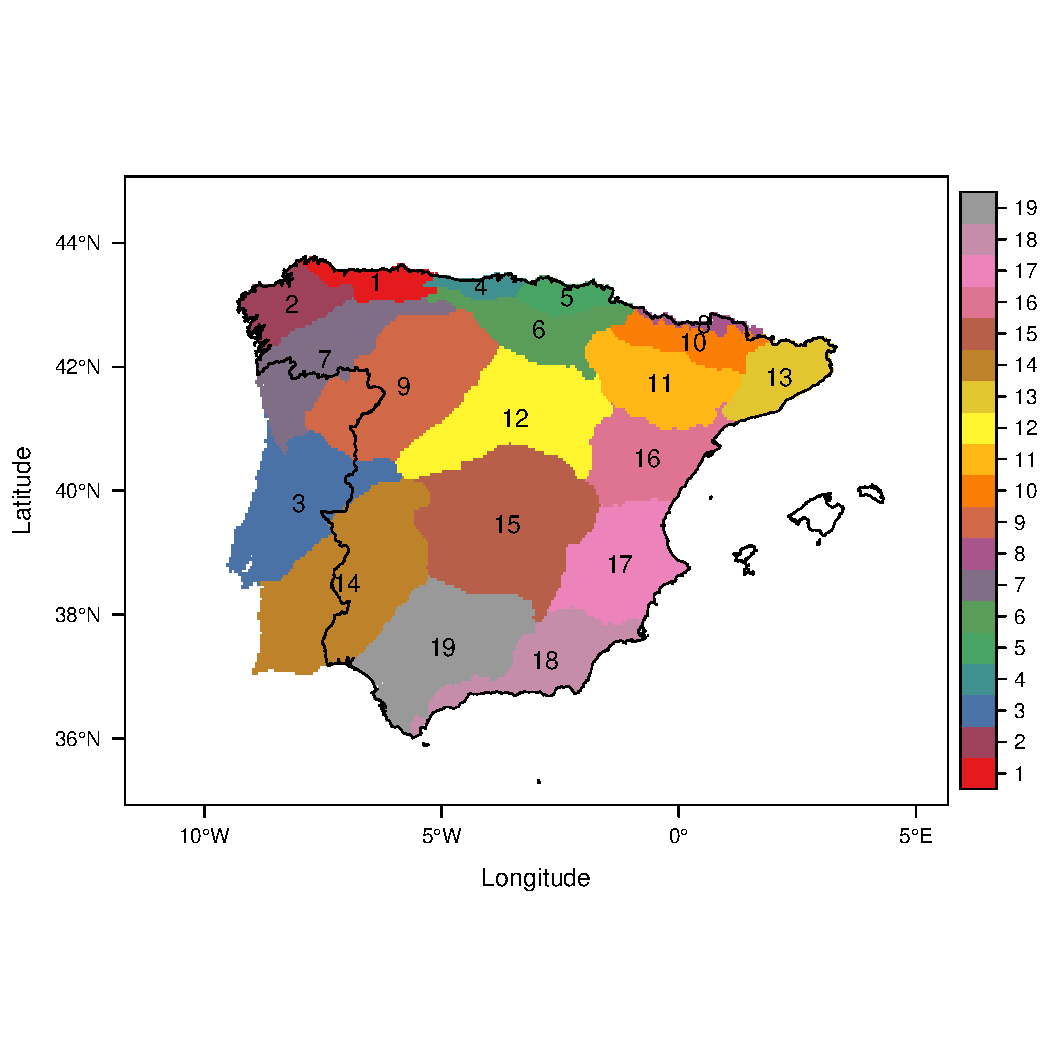
\includegraphics[scale=0.2]{clusters2.pdf}
%       \end{figure}
      \begin{itemize}
      \item Ratio: \begin{math} {CV_{productivity}}\over{CV_{G0}}\end{math}
     \item Linear relationship: Ratio and cluster.  
      \item $Ratio > 1$ %: variability of PV productivity is higher
        \begin{itemize}
        \small{\item For tracking systems, whole year.
        \item All systems in winter months.}
        \end{itemize} 
        \item $Ratio < 1$ %: variability of PV productivity is lower
        \begin{itemize}
        \small{\item For fixed systems in summer months.}
        \end{itemize}  
      \end{itemize}  
    \end{column}
  \end{columns}
\end{frame}

% \begin{frame}[fragile]{Results: complementarity}
% \begin{figure}
%   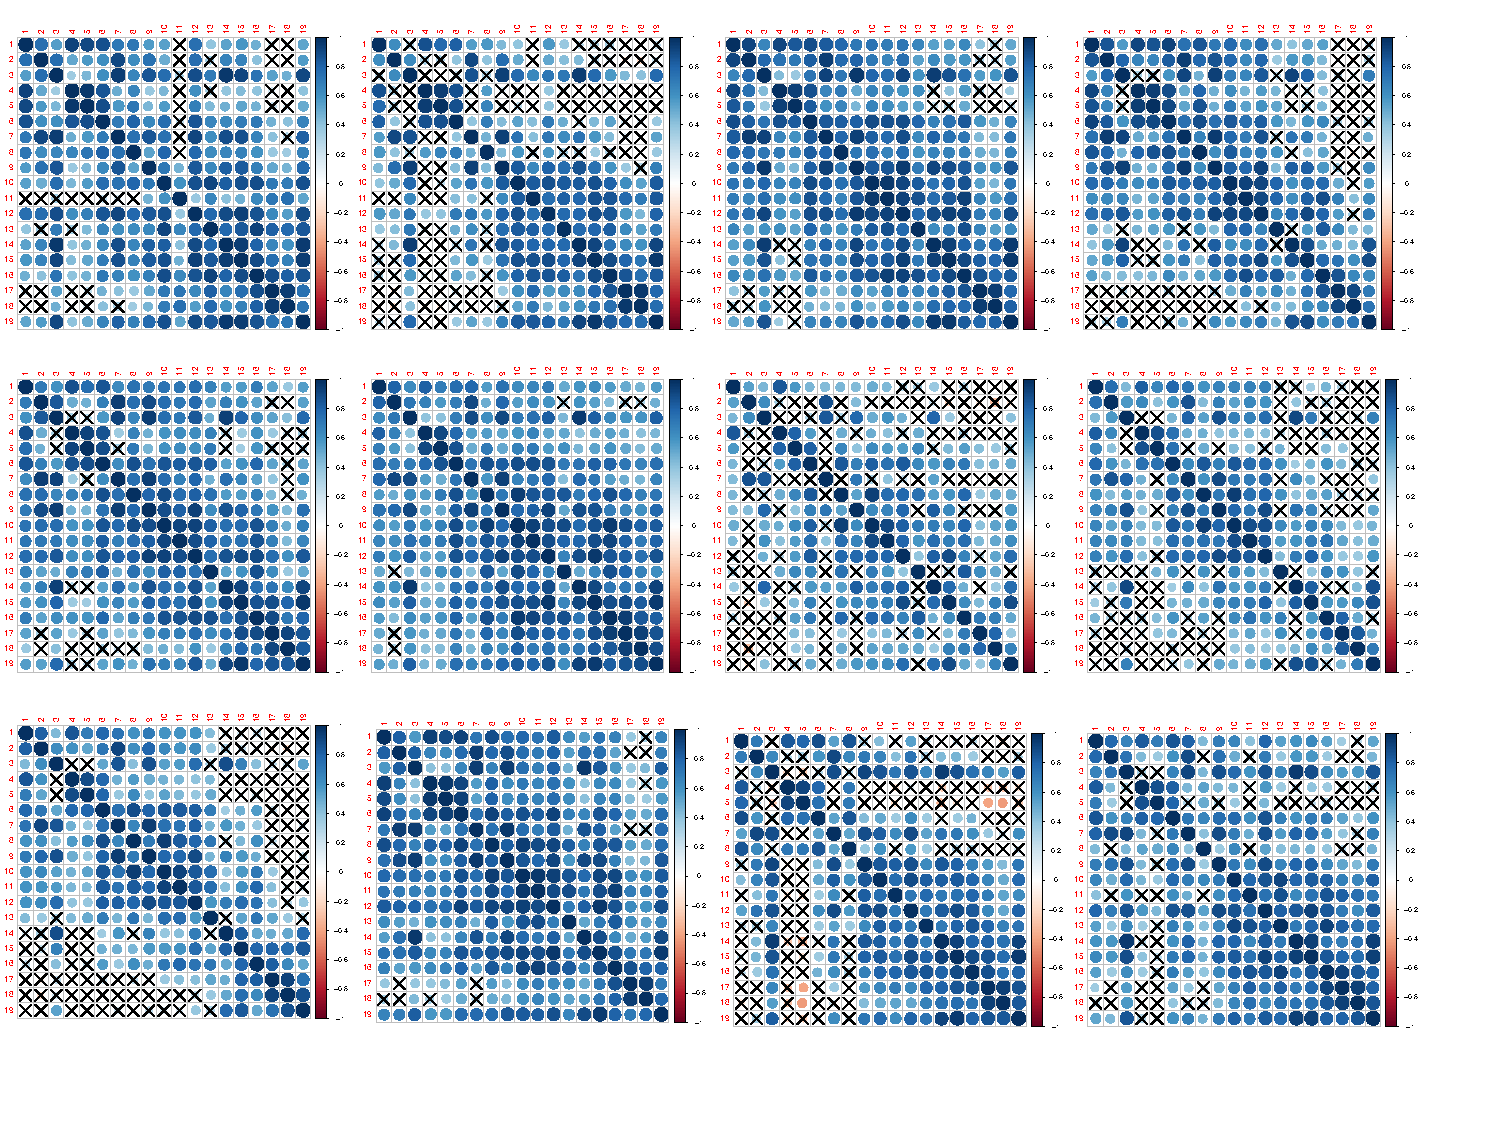
\includegraphics[scale=0.42]{correlaciones_30.pdf}
%   \end{figure}
% \end{frame}

\begin{frame}[fragile]{Results: complementarity}
  \begin{columns}
    \begin{column}{0.6\textwidth}
      \begin{figure}
        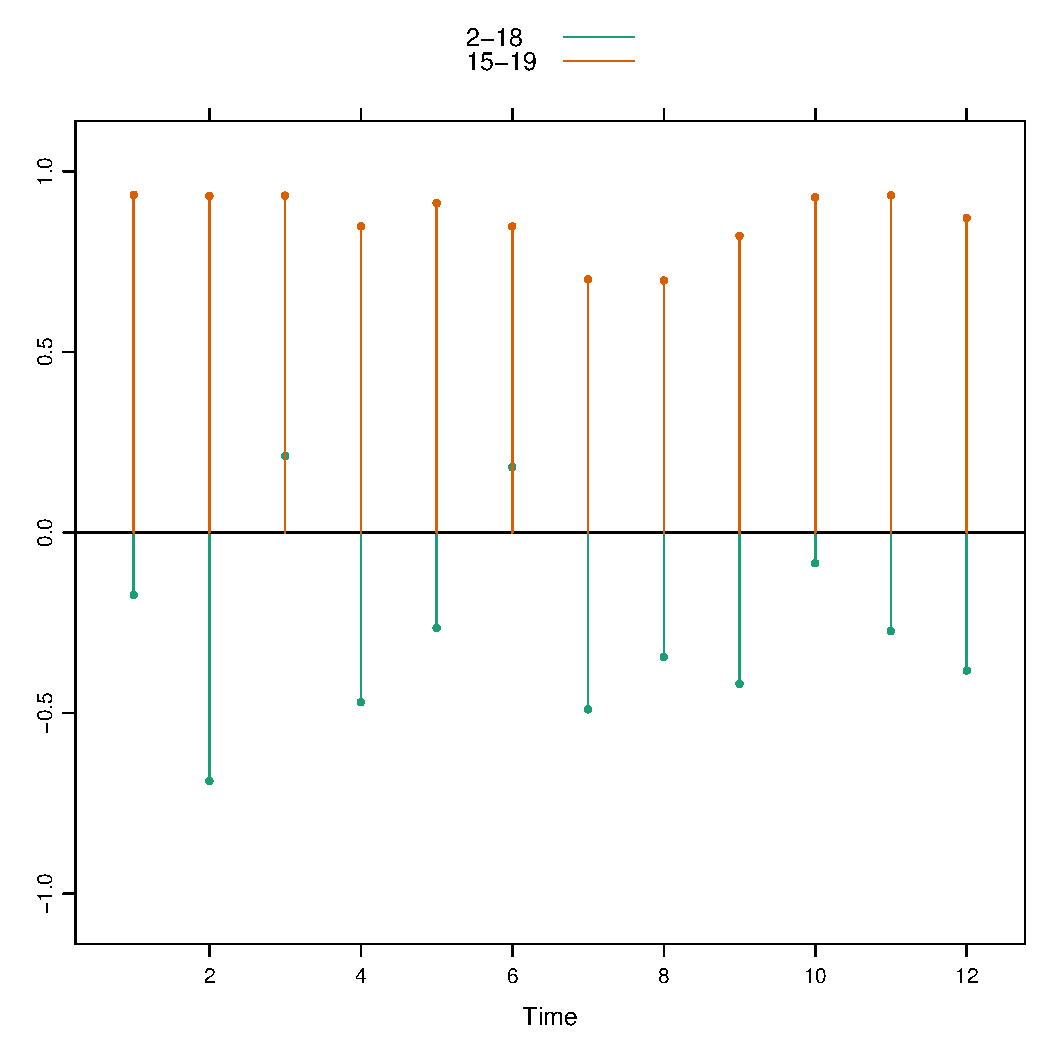
\includegraphics[scale=0.37]{figure9.pdf}
\centering{\caption{Most (2-19) and less important (15-19) cluster pairs for complementarity}}
      \end{figure}
\end{column}
    \begin{column}{0.5\textwidth}
%       \begin{figure}
% \hspace{1.5\baselineskip}{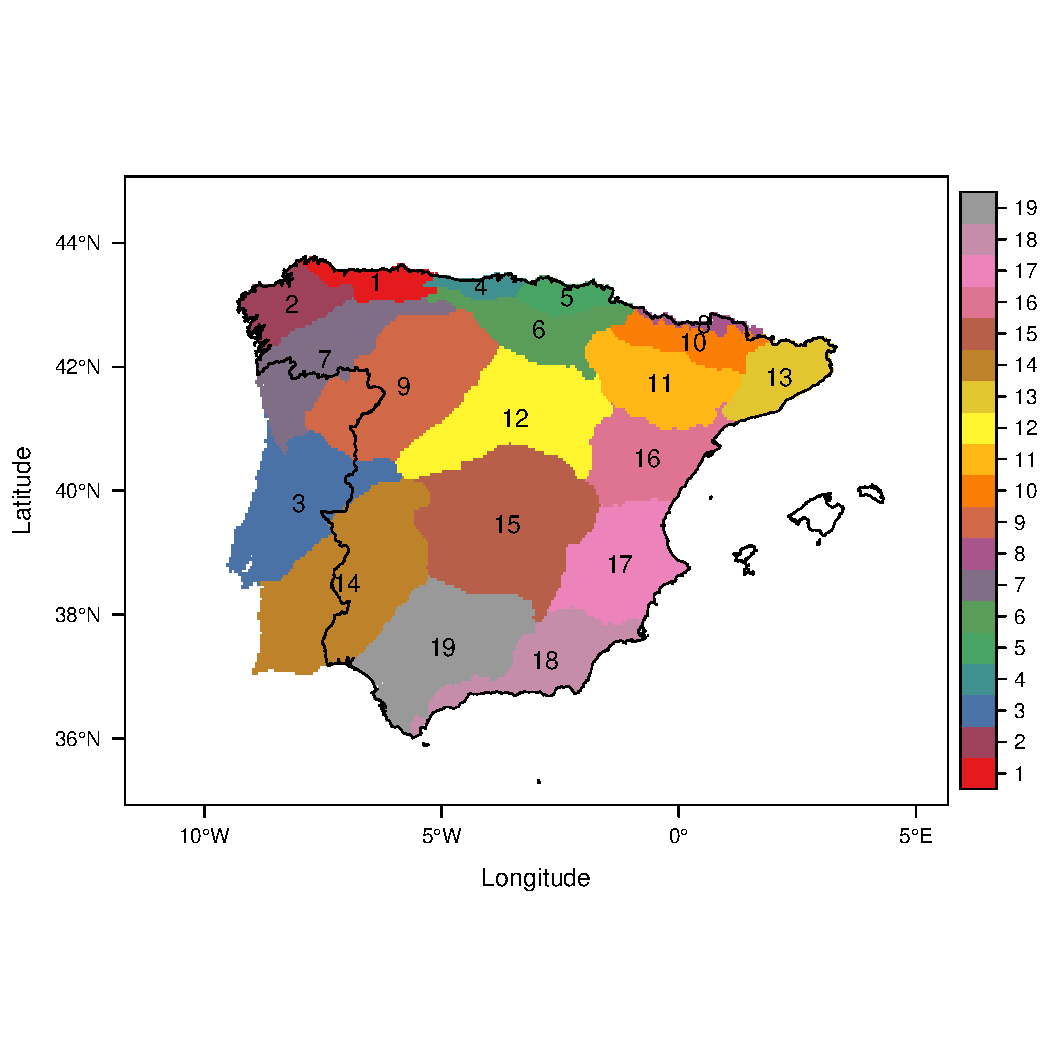
\includegraphics[scale=0.2]{clusters2.pdf}
%       \end{figure}
      \begin{itemize}
      \item \textbf{2-18}: North-West/South-East negative correlated.
      \item Values varies among the year.
      \item Some pairs are highly correlated.
      \end{itemize}  
    \end{column}
  \end{columns}
\end{frame}

\begin{frame}[fragile]{Conclusions}
    \begin{itemize}
    \item<1->  The clustering algorithm is able to detect sub-regions with different characteristics.
    \item <2->The tracking system is important when considering variability between clusters.
    \item <3->The variability analysis shows a stable year-to-year resource, but with differences between areas.
    \item <4->The complementarity results show:
      \begin{itemize}
      \item For the monthly series, most clusters are correlated but there is certain grade of complementarity between clusters in the Atlantic coast and the South East of the IP.
      \end{itemize}
    \item <5->The multi-step scheme is flexible for different variables and scales.  
    \end{itemize}
\end{frame}

\section{Results. Part II}


\begin{frame}[standout]
\centering{Impact of aerosols on photovoltaic energy production over the Euro-Mediterranean area\footnote{\tiny{\textcolor{white}{This chapter has been published as a paper in Solar Energy journal; doi:}}}}
\end{frame}

\begin{frame}[fragile]{Introduction}
\textbf{\alert{Aerosols}} are an important source of \textbf{variability} of solar radiation over the \textbf{Euro-Mediterranean} area. 
\small{  \begin{itemize}
\item<2->  They impact solar radiation \textbf{directly} and \textbf{indirectly}.
\item<2->  In \textbf{low frequency} variability (decadal changes) the role of aerosols has been studied over Europe (\textbf{dimming/brightrenning}) 
\item<2->  However: most of the RCMs do \textbf{not include aerosols} on their simulations.
\end{itemize}}
\end{frame}

\begin{frame}[fragile]{Objective}
To assess the \textbf{\alert{impact}} of \textbf{aerosols} on \textbf{photovoltaic} energy production over the Euro-Mediterranean area.
\small{  \begin{itemize}
  \item From seasonal to multi-decadal time scales.
  \item Are regional climate models useful for the renewable energy resource assessment studies?
  \end{itemize}}
\end{frame}

\begin{frame}[fragile]{Data and Methods}
  \textbf{Climate data}\\
\vspace{0.5\baselineskip}
  \begin{columns}
    \begin{column}{0.5\textwidth} 
{RCM: \textbf{\alert{CNRM-RCSM4}}}
  \begin{table}
    {\tiny{
    \centering{\begin{tabular}[1\textwidth]{c|c|c|c}
      \toprule
      Simulation & Aerosols & Period \\
                 \midrule
                 AER & NAB13 & 2003-2009 \\
                 NO-AER & Not included & 2003-2009\\
                 TREND & NAB13 + sulfates trend & 1980-2012
      \bottomrule
               \end{tabular}}
\vspace{0.5\baselineskip}{\caption{summary of simulations}}
           \end{table}}}
     \end{column}
     \begin{column}{0.5\textwidth}
       \begin{figure}
       \vspace{0.2\baselineskip}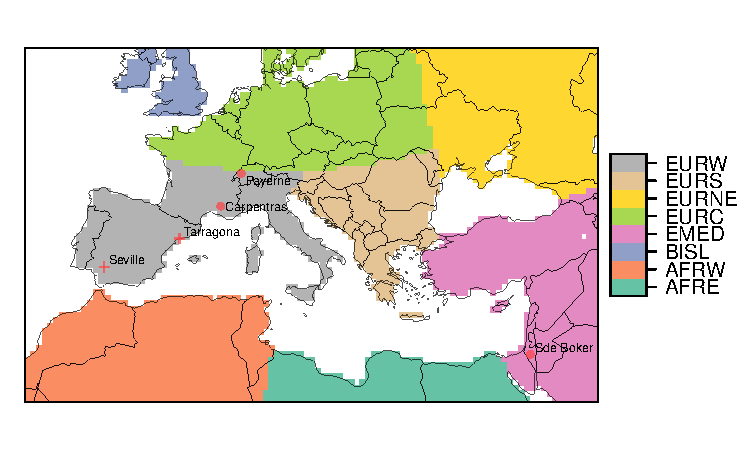
\includegraphics[scale=0.4]{zonasPuntosLabel.pdf}
       \end{figure}
     \end{column}
     \end{columns}
       \textbf{Measurements}
       \begin{columns}
         \begin{column}{0.5\textwidth}
       \begin{itemize}
       \item Solar radiation: \textbf{\alert{BSRN}}
       \end{itemize}
  \begin{table}
    {\tiny{
    \centering{\begin{tabular}[1\textwidth]{c|c|c|c}
      \toprule
      Station & Time resolution & Period \\
                 \midrule
                 Payerne & monthly & 2003-2009 \\
                 Sede-Boker & monthly & 2003-2009\\
                 Carpentras & monthly & 2003-2009\\
      \bottomrule
               \end{tabular}}
             \vspace{0.75\baselineskip}
             \caption{summary of stations}
           \end{table}}}
     \end{column}
     \begin{column}{0.5\textwidth}
       \begin{itemize}
       \item \textbf{\alert{PV}} production \textbf{\alert{data}}:
       \end{itemize}
       \begin{table}
    {\tiny{
    \centering{\begin{tabular}[1\textwidth]{c|c|c|c}
      \toprule
      PV plant & Type & Period \\
                 \midrule
                 Seville & fixed & daily: 2-07-2007/30-11-2008 \\
                 Tarragona & Two-axes & daily: 01-01-2003/19-03-2005\\
      \bottomrule
               \end{tabular}}
             \vspace{0.75\baselineskip}
             \caption{PV plants}
           \end{table}}}
     \end{column}
     \end{columns}
\end{frame}

\begin{frame}[fragile]{Results: Local scale}
  \textbf{SSR}\\
  \begin{table}
  {\tiny{
    \centering{\begin{tabular}[1.5\textwidth]{c|c|c|c|c|c}
      \toprule
      Location & Simultation & RMSE & MBE & cor & sd \\
                 \midrule
               & AER & 16.59 & 12.05 & 0.98 & 90.05\\
               Carpentras & NO-AER & 27.26 & 24.10 & 0.99 & 90.57\\
               & SAT & 6.38 & 4.26 & 1.00  & 8.71\\
                 \midrule
               & AER & 21.21 & 16.62 & 0.97 & 77.40\\  
               Payerne & NO-AER & 29.70 & 27.07 & 0.98 &81.88\\
               & SAT & 7.36 & 4.60 & 0.99 & 83.29 \\
               \midrule  
               & AER & 18.89 & 8.17 & 0.98 & 62.83\\  
               Sede Boker & NO-AER &37.42 &35.63 &0.98 &76.06\\
               & SAT & 12.00 & 10.27 & 0.99 & 77.62 \\
                 \bottomrule
               \end{tabular}}
             \vspace{0.75\baselineskip}
             \caption{Evaluation of SSR from simulations}
           \end{table}}}
  % \begin{figure}
  %   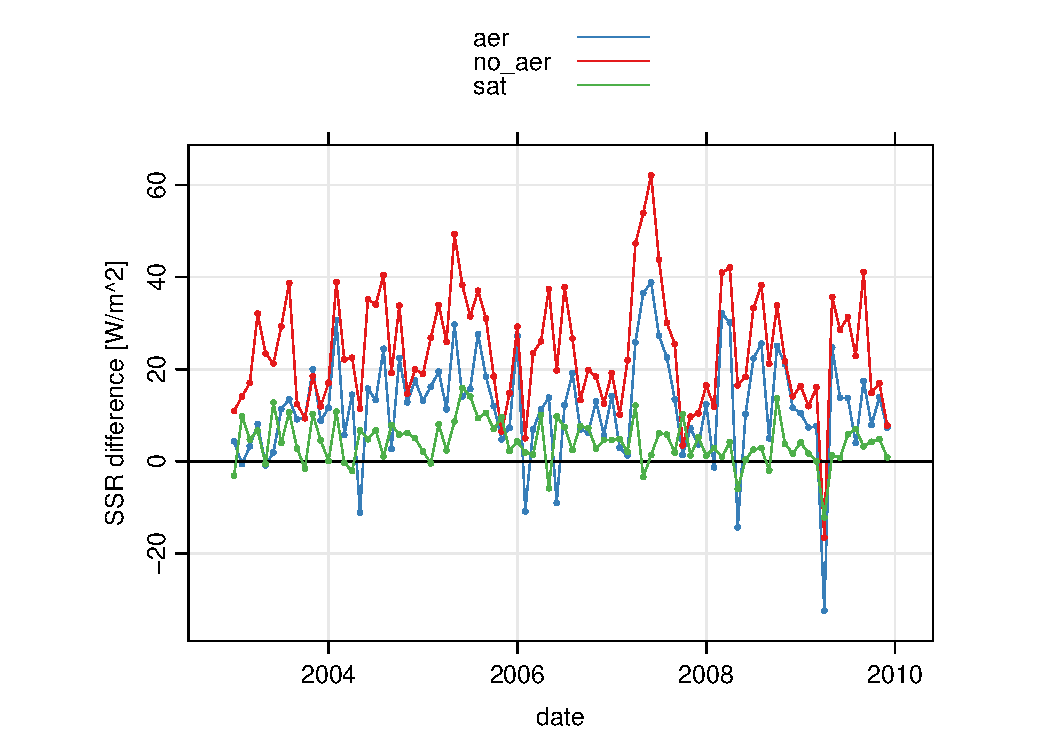
\includegraphics[scale=0.22]{CarpentrasMesesDif.pdf}
  %   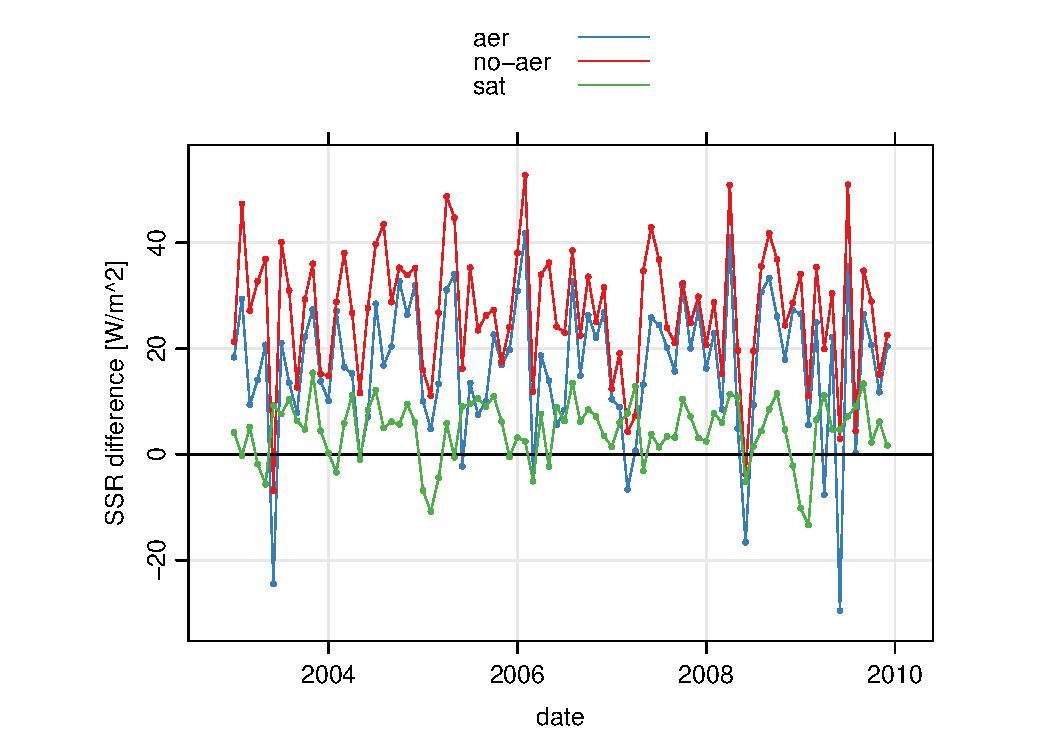
\includegraphics[scale=0.22]{PayerneMesesDif.pdf}
  %   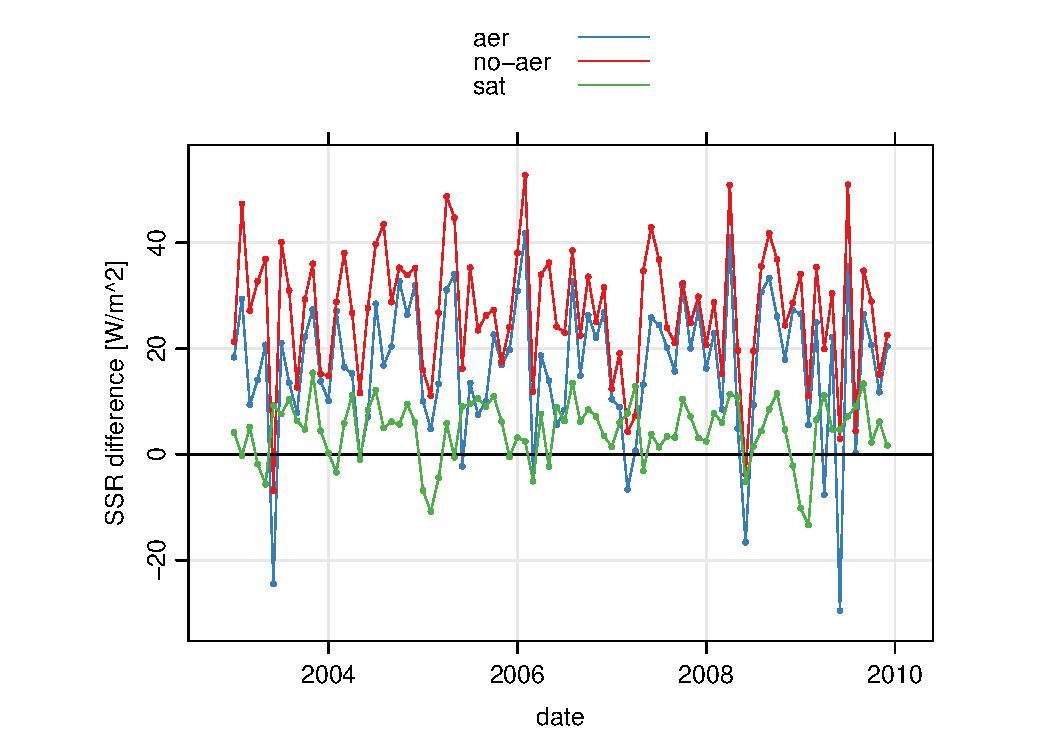
\includegraphics[scale=0.22]{SedebokerMesesDif.pdf}
  %   \end{figure}
\end{frame}

\begin{frame}[fragile]{Results: Local scale}
  \textbf{PV production}\\
  \vspace{0.5\baselineskip}
  \begin{columns}
    \begin{column}{0.8\textwidth}
  \hspace{3.2\baselineskip}{Seville}
  \hspace{3.8\baselineskip}{Tarragona}
  \begin{figure}
    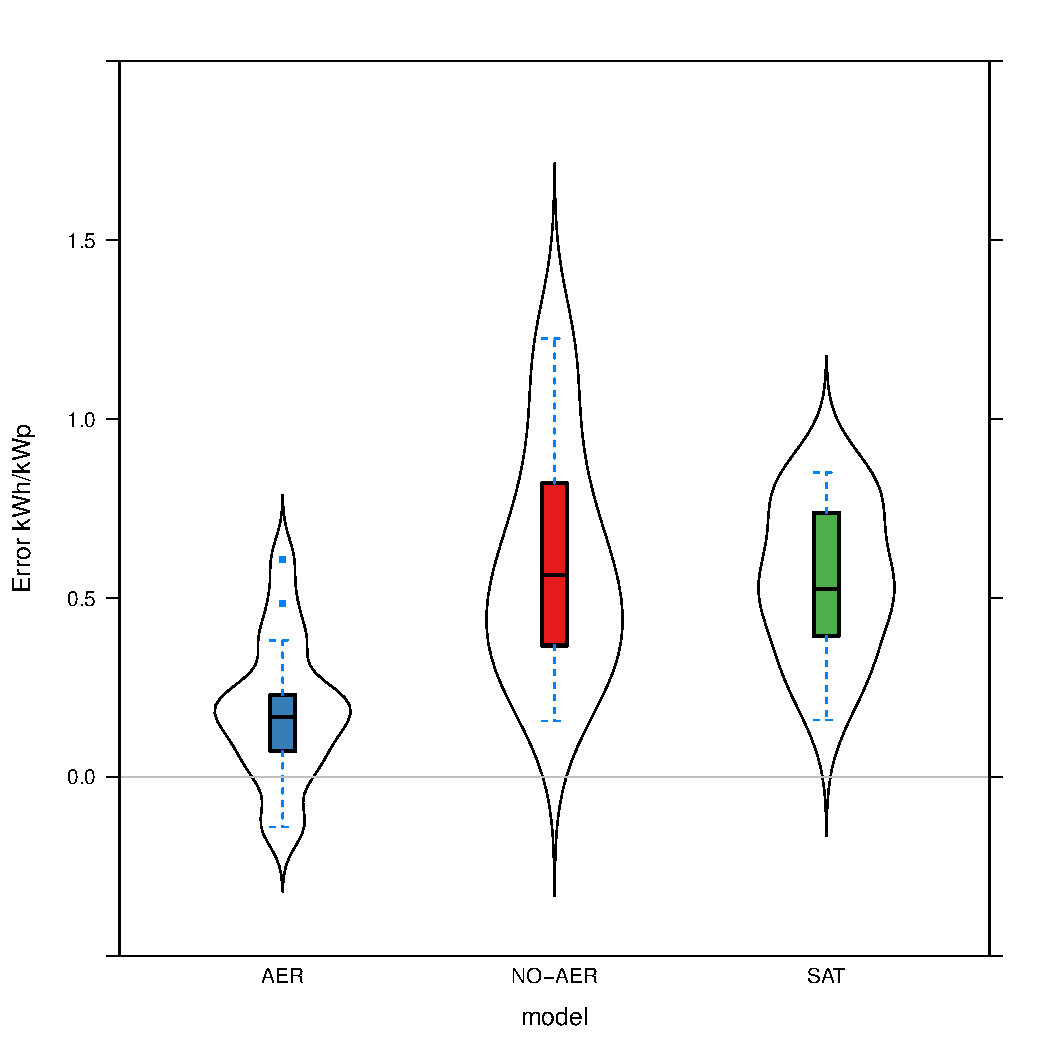
\includegraphics[scale=0.2]{violinplorSeville.pdf}
    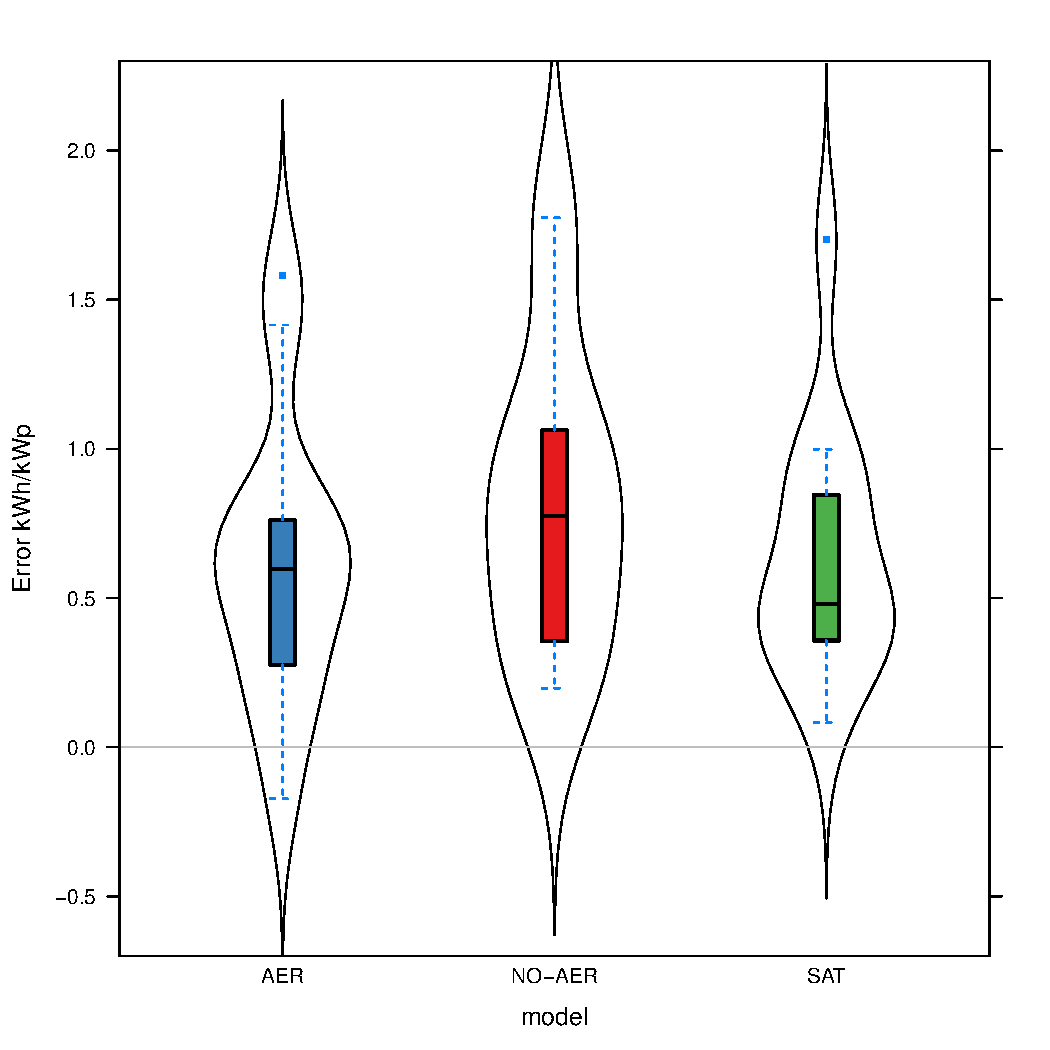
\includegraphics[scale=0.2]{violinplotTarragona.pdf}
  \end{figure}
\end{column}
\begin{column}{0.2\textwidth}
  \tiny{{\textcolor{blue}{NO-AER}}}\\
  \tiny{{\textcolor{red}{AER}}}\\
  \tiny{{\textcolor{green!90}{SAT}}}\\
\end{column}
\end{columns}
{\small{\begin{itemize}
\item For Seville PV plant, AER performs better than NO-AER and SAT.
\item Higher errors are found in Tarragona plant for all the simulations. 
\item NO-AER is the one with higher errors in both cases.
\end{itemize}}}  
\end{frame}

\begin{frame}[fragile]{Results: Regional scale}
\textbf{SSR}: Simulation-Satellite  
  \begin{figure}
  \includegraphics[scale=0.5]{dif_model_sat_zonas}%diferencia_mesesFIXED2.png}  
\end{figure}
\begin{itemize}
\item The NO-AER overestimates in comparison with SAT.
\item Small interannual variability.
\item AER underestimates in AFRW  
\end{itemize}
\end{frame}

\begin{frame}[fragile]{Results: Impact of aerosols by tracking type}
\textbf{Mean behavior: 2003-2009}
  \begin{figure}
  \includegraphics[scale=0.3]{byCountry}  
\caption{Relative difference [\textbf{\%}]of PV productivity averaged by country and by type}
\end{figure}
\begin{itemize}
\item a
\item b
\item c  
\end{itemize}
\end{frame}

\begin{frame}[fragile]{Results: Impact of aerosols by tracking type}
  \begin{columns}
  \begin{column}{0.7\textwidth}
    \begin{figure}
\small{\textbf{Seasonal cycle: 2003-2009}}
  \includegraphics[scale=0.5]{seasonalimpact.pdf}  
\end{figure}
\end{column}
\begin{column}{0.43\textwidth}
\begin{itemize}
\item a
\item b
\item c  
\end{itemize}
\end{column}
 \end{columns}
\end{frame}

\begin{frame}[fragile]{Results: Impact of aerosols by tracking type}
\small{\textbf{Long-term trends: 1980-2012}}
\begin{figure}
\includegraphics[scale=0.38]{longterm.pdf}  
\end{figure}
\begin{itemize}
\item a
\item b
\item c
\end{itemize}  
\end{frame}

\begin{frame}[fragile]{Conclusions}
\textbf{\alert{Discussion}}
{\small{  \begin{itemize}
\item Limitations due to the RCM: single model, horizontal resolution, time resolution of aerosols, cloud representation. 
\item PV production data: a need for real PV production data would help on the modeling chain assessment.
\end{itemize}}}
\textbf{\alert{conclusions}}
{\small{\begin{itemize}
\item The RCM simulations are able to reproduce real data of two PV plants.
\item The RCM with aerosols improves with respect to the no-aerosols.
\item The impact of aerosols has been quantify with a sensitivity test:
  \begin{itemize}
  \item most impacted areas in central Europe.
  \item In the multi-decadal...
  \end{itemize}
\end{itemize}}}  
\end{frame}

\section{Results. Part III}
 
\begin{frame}[fragile]{SSR mean changes 2021-2050}
\vspace{1\baselineskip}
\begin{columns}
  \begin{column}{0.45\textwidth}
    \centering{\hspace{3\baselineskip}\LARGE{\textbf{GCM}}}
      \end{column}
      \begin{column}{0.7\textwidth}
        \hspace{5.4\baselineskip}{\LARGE{\textbf{RCM}}}
   \end{column}
   \end{columns}
    \begin{figure}
      \includegraphics[scale=0.32]{ssr_gimp4.png}
        \centering\caption{SSR change (1971/2000)-(2021/2050) ($W/m^2$)}
      \end{figure}
\end{frame}

\begin{frame}[fragile]{SSR mean changes 2021-2050}
\vspace{0.5\baselineskip}
\begin{columns}
  \begin{column}{0.7\textwidth}
 \hspace{1.8\baselineskip}\LARGE{\textbf{GCM}}
   %    \end{column}
   %    \begin{column}{0.7\textwidth}
      \hspace{4\baselineskip}{\LARGE{\textbf{RCM}}}
   % \end{column}
   % \end{columns}
    \begin{figure}
      \includegraphics[scale=0.26]{ssr_gimp3.png}
        \centering\caption{SSR change (1971/2000)-(2021/2050) ($W/m^2$)}
    \end{figure}
  \end{column}
  \begin{column}{0.4\textwidth}
    \begin{itemize}
      \centering\item Only RCMs with evolving aerosols show the increase in SSR as GCMs.
    \end{itemize}
  \end{column}
  \end{columns}
\end{frame}
 
% \begin{frame}[fragile]{SSR mean changes 2021-2050}
% \vspace{0.5\baselineskip}
% \begin{columns}
%   \begin{column}{0.45\textwidth}
% \hspace{4\baselineskip}\centering{\LARGE{\textbf{GCM}}}
%       \end{column}
%       \begin{column}{0.7\textwidth}
%         \hspace{5.2\baselineskip}{\LARGE{\textbf{RCM}}}
%    \end{column}
%    \end{columns}
%     \begin{figure}
%       \includegraphics[scale=0.3]{ssr_gimp3.png}
%         %\centering\caption{SSR change (1971/2000)-(2021/2050) ($W/m^2$)}
%     \end{figure}
% %    \vspace{0.01\baselineskip}
%       \begin{itemize}
%       \item Only RCMs with evolving aerosols show the increase in SSR as GCMs.
%         \end{itemize}
% \end{frame}

\begin{frame}[fragile]{CLT mean changes 2021-2050}
\vspace{1\baselineskip}
\begin{columns}
  \begin{column}{0.4\textwidth}
    \centering{\hspace{5.2\baselineskip}\LARGE{\textbf{GCM}}}
      \end{column}
      \begin{column}{0.7\textwidth}
        \hspace{6\baselineskip}{\LARGE{\textbf{RCM}}}
   \end{column}
   \end{columns}
    \begin{figure}
      \includegraphics[scale=0.3]{clt_gimp3.png}
        \centering\caption{CLT change (1971/2000)-(2021/2050) ($\%$)}
      \end{figure}
\end{frame}
 
\begin{frame}[fragile]{CLT mean changes 2021-2050}
\vspace{1\baselineskip}
\begin{columns}
  \begin{column}{0.7\textwidth}
    \hspace{2\baselineskip}\LARGE{\textbf{GCM}}
%      \end{column}
%      \begin{column}{0.7\textwidth}
        \hspace{3.8\baselineskip}{\LARGE{\textbf{RCM}}}
%   \end{column}
%   \end{columns}
    \begin{figure}
      \includegraphics[scale=0.26]{clt_gimp3.png}
        \centering\caption{CLT change (1971/2000)-(2021/2050) ($\%$)}
    \end{figure}
  \end{column}
  \begin{column}{0.4\textwidth}
      \begin{itemize}
        \centering\vspace{0.05\baselineskip}\item RCMs without evolving aerosols: CLT spatial pattern can explain SSR spatial pattern.
        \centering\item CLT spatial pattern cannot explain SSR spatial pattern in models with evolving aerosols.
      \end{itemize}
    \end{column}
    \end{columns}
\end{frame}

% \begin{frame}[fragile]{CLT mean changes 2021-2050}
% %\vspace{1\baselineskip}
% \begin{columns}
%   \begin{column}{0.45\textwidth}
%     \centering{\hspace{4\baslineskip}\LARGE{\textbf{GCM}}}
%       \end{column}
%       \begin{column}{0.7\textwidth}
%         \hspace{5.2\baselineskip}{\LARGE{\textbf{RCM}}}
%    \end{column}
%    \end{columns}
%     \begin{figure}
%       \includegraphics[scale=0.3]{clt_gimp2.png}
%         \centering\caption{CLT change (1971/2000)-(2021/2050) ($\%$)}
%       \end{figure}
%     \vspace{0.01\baselineskip}
%       \begin{itemize}
%       \item No clear relationship between SSR and CLT.
%       \end{itemize}
% \end{frame}


\begin{frame}[fragile]{Mean changes 2021-2050}
  \begin{table}
    {\small{
    \centering{\begin{tabular}[1\textwidth]{c|c|c|c}
      \toprule
      GCM & RCM & $\Delta{SSR}$ [$W/m^2$] & $\Delta{CLT}$ [$\%$]\\
                 \midrule
                 CNRM-CM5 &  & \textbf{9.9} & 0.5\\
                & CCLM4-8-17 & -2.4& -0.8 \\
                & \alert{ALADIN53} & \textbf{12.6}& 0.3\\
                & RCA4 & -2.6 & 0.2 \\
                 \midrule
                 EC-EARTH & & \textbf{5.6}& -0.3\\
                & CCLM4-8-17 & -2.7 & -0.9\\
                & \alert{RACMO22E} & \textbf{4.8}& 0.5\\
                & RCA4 & -2.1 & 0.1\\
      \bottomrule
               \end{tabular}}
             \vspace{0.75\baselineskip}
             \caption{Spatial changes in SSR and CLT}
     \end{table}}}
\end{frame}

\begin{frame}[fragile]{AOD mean changes 2021-2050}
  \begin{columns}
   \begin{column}{0.5\textwidth}
      \begin{figure}
         \centering\includegraphics[scale=0.5]{aod.png}
     \centering\caption{AOD change (1971/2000)-(2021/2050)}
   \end{figure}
     \end{column}
     \begin{column}{0.6\textwidth}
       \begin{itemize}
       \item Spatial pattern of $\Delta{AOD}$ similar to $\Delta{SSR}$ when evolving aerosols considered.
       \item Higher correltation of SSR with AOD than with CLT.
       \end{itemize}
     \end{column}
   \end{columns}   
  \begin{table}
    {\tiny{
    \centering{\begin{tabular}[1\textwidth]{c|c|c|c|c}
      \toprule
      GCM & RCM & $\Delta{AOD}$ & $\rho_{SSR,CLT}$ & $\rho_{SSR,AOD}$\\
                 \midrule
                & CCLM4-8-17 & - & -0.7 & -\\
                CNRM-CM5& \alert{ALADIN53} & -0.2 & -0.2& -0.9 \\
                & RCA4 & - & -0.8& -\\
                 \midrule 
                & CCLM4-8-17 & - & -0.8 & - \\
                EC-EARTH& \alert{RACMO22E} & -0.1 & -0.3 & -0.6\\
                & RCA4 & - & -0.8 & -\\
      \bottomrule
               \end{tabular}}
           \end{table}}}
\end{frame}
 

\subsection{$\Delta{PV}$ by country}
 
\begin{frame}[fragile]{$\Delta$PV relative JJA mean by country}
     \begin{figure}
       \centering\includegraphics[scale=0.65]{bycountryJJArelative_area_newscriptall5}
       \caption{Relative change in PV potential [\%]}
     \end{figure}
\end{frame}

% \begin{frame}[fragile]{$\Delta$PV relative JJA mean by country}
%   \vspace{0.5\baselineskip}
%      \begin{figure}
%        \centering\includegraphics[scale=0.5]{bycountryJJArelative_area_newscriptall5_2}
%        \centering\caption{Relative change in PV potential [\%]}
%      \end{figure}
%      \begin{itemize}
%      \item Decrease for models with no-evolving aerosols  
%        \end{itemize}
% \end{frame}

\begin{frame}[fragile]{$\Delta$PV relative JJA mean by country}
  \vspace{0.5\baselineskip}
  \begin{columns}
    \begin{column}{0.6\textwidth}
  \begin{figure}
       \centering\includegraphics[scale=0.5]{bycountryJJArelative_area_newscriptall5_2}
       \centering\caption{Relative change in PV potential [\%]}
     \end{figure}
   \end{column}
   \begin{column}{0.4\textwidth}
     \begin{itemize}
     \item Decrease for models with no-evolving aerosols.
     \end{itemize}
     \end{column}
     \end{columns}
\end{frame}

\begin{frame}[fragile]{$\Delta$PV relative JJA mean by country}
  \vspace{0.5\baselineskip}
  \begin{columns}
    \begin{column}{0.6\textwidth}
  \begin{figure}
       \centering\includegraphics[scale=0.5]{bycountryJJArelative_area_newscriptall5_3}
       \centering\caption{Relative change in PV potential [\%]}
     \end{figure}
   \end{column}
   \begin{column}{0.4\textwidth}
     \begin{itemize}
     \item Decrease for models with no-evolving aerosols.
     \item Increase for models with evolving aerosols.
     \item Central-Europe is the most impacted area.  
     \end{itemize}
     \end{column}
     \end{columns}
\end{frame}

% \begin{frame}[fragile]{}
%   \begin{figure}
%     {\alert{Anomalía de radiación (JJA) 2050/2021-2000/1971}}
%         \centering\includegraphics[scale=0.55]{diferences_ssr_newperiods_9abr.pdf}\\
%         %\centering\includegraphics[scale=0.45]{diferences_clt_newperiods_9abr.pdf}
%         \tiny{\centering\caption{Anomal\'ia de radiaci\'on en superficie (2021/2050)-(1971/2000) ($W/m^2$)}}
%       \end{figure}
%       \begin{itemize}
%       \item <1->Diferentes patrones espaciales en la anomal\'ia
%       \item <1->CNRM-ALADIN5.3 presenta incremento generalizado
%       \end{itemize}
% \end{frame}

% \begin{frame}[plain]{RCP4.5}
%   \begin{figure}
%     {\alert{Anomalía de nubosidad (JJA) 2050/2021-2000/1971}}
%       \centering\includegraphics[scale=0.55]{diferences_clt_newperiods_9abr.pdf}
%      \centering\caption{Anomal\'ia de la cubierta nubosa  (2021/2050)-(1971/2000) for ALADIN5.3 ($\%$)}
%    \end{figure}
%    \begin{itemize}
%    \item Descenso de la nubosidad.
%    \item Correlaci\'on espacial entre SSR y CLT mayor para ENEA-PROTHEUS (-0.6 vs -0.9).  
%    \end{itemize}
% \end{frame}

% \begin{frame}[fragile]{RCP4.5}
% Anomal\'ias para todo el dominio de ambas variables:  
%  \begin{table}
%     \caption{Simulaciones de RCM utilizadas}
%     \begin{tabular}{c|c|c}
%       \toprule
%       Modelo & SSR [$W/m^2$] & CLT [$\%$] \\
%       \midrule
%       ENEA-PROTHEUS & 0.67 & -1.76 \\
%       CNRM-ALADIN5.3 & 6.83 & -1.17\\
%       \bottomrule
%     \end{tabular}
%   \end{table}  
% \end{frame}

\section{Conclusions}

\begin{frame}[fragile]{Conclusions}
\begin{alertblock}{}
    \begin{itemize}
    \item  For the mid century, an \textbf{\alert{increase}} in \textbf{photovoltaic potential} is projected over Europe when the \textbf{evolution} of \textbf{aerosols} over the area is considered.
    \item The \textbf{magnitude} depends on the country and the models.
    \item The most impacted areas are in Central-Europe, with an important potential increase of more than \textbf{10\%} but large uncertainty between models.
    \end{itemize}
\end{alertblock}
\begin{alertblock}{Perspectives}
\begin{itemize}
\item A \textbf{robust answer} is needed in order to deliver key messages for the solar industry.
\item The FPS-aerosols could help to understand uncertainties and develop better projections for energy purposes.  
% \item  La representación de los aerosoles en las \textbf{proyecciones de CC.} influyen en las variables relevantes para el potencial fotovoltaico.
\end{itemize}
\end{alertblock}
\end{frame}

% \begin{frame}{Perspectivas}
% \begin{alertblock}{Análisis multimodelo EURO-CORDEX}
% Estudio de la influencia de los aerosoles en escenarios de CC. sobre la radiación y la producción fotovoltaica con un 'ensemble' de modelos.
% \end{alertblock}
% \begin{alertblock}{}
%   \begin{itemize}
% \item Resultados robustos sobre la \textbf{evoluci\'on} del recurso solar. 
% \item Importancia en el desarrollo de los \textbf{servicios clim\'aticos}.
% \end{itemize}
% \end{alertblock}
% \end{frame}

\begin{frame}[standout]
    Thank you for your attention.\\ 
\vspace{2\baselineskip}\small{claudia.gutierrez@uclm.es}
\end{frame}

\end{document}


            
